\RequirePackage{fix-cm}
\documentclass[oneside]{report}

% Biên dịch bằng XeLaTeX + BibTeX hoặc Tectonic.
\usepackage[no-math]{fontspec}
\newcommand{\ThesisTitle}{Longitudinal Learning with Tensor Fusion for Predicting Progression of Alzheimer’s Disease}
\newcommand{\ThesisTitleVN}{Học trên dữ liệu theo dõi dọc với hợp nhất tensor để dự đoán tiến triển bệnh Alzheimer}
\title{\ThesisTitle}
\author{Nguyễn Phương Nam}
\date{2026}
% Cùng family và weight với bản mẫu Nguyễn Phương Trang.
% Dùng tên file OpenType từ TeX distribution, không cần cài font hệ thống.
\setmainfont{LibertinusSerif}[
  Extension=.otf,
  UprightFont=*-Regular,
  BoldFont=*-Semibold,
  ItalicFont=*-Italic,
  BoldItalicFont=*-SemiboldItalic
]
% Giữ các family Latin Modern mặc định cho sans-serif/monospace như bản mẫu.

% Cùng lề trang với bản mẫu Nguyễn Phương Trang: A4, trái 3 cm,
% phải 2 cm, trên 2 cm, dưới 2.5 cm; chữ 13 pt, giãn dòng 1.3.
\usepackage[a4paper,left=30mm,right=20mm,top=20mm,bottom=25mm]{geometry}
\usepackage{graphicx}
\usepackage{pdflscape}
\graphicspath{{image/}{figures/}}
\usepackage{tikz}
\usetikzlibrary{arrows.meta,positioning,calc,fit,backgrounds,shapes.geometric,matrix}
\usepackage{xcolor}
\definecolor{uetblue}{HTML}{0B4F78}
\definecolor{softblue}{HTML}{DCEEFF}
\definecolor{softgreen}{HTML}{E2F3E7}
\definecolor{softorange}{HTML}{FCE8D5}
\definecolor{softpurple}{HTML}{EAE2F3}
\definecolor{softgray}{HTML}{F3F4F6}
\definecolor{darkgreen}{HTML}{247A3C}
\definecolor{darkorange}{HTML}{B85C00}

\usepackage{amsmath,mathtools}
% Keep OpenType text encoding for operators; OT1 has no LibertinusSerif family.
\usepackage[noOT1]{newtxmath}
\usepackage{bm}
\usepackage{booktabs,tabularx,longtable,multirow,array}
\usepackage{float}
\floatstyle{ruled}
\newfloat{algorithm}{htbp}{loa}
\floatname{algorithm}{Thuật toán}
\floatstyle{plain}
\usepackage{caption}
\usepackage{subcaption}
\captionsetup{font=normalsize,labelfont=normalfont,textfont=normalfont,skip=6pt}
\usepackage{enumitem}
\usepackage{listings}
\usepackage{microtype}
\usepackage{scrextend}
\usepackage{indentfirst}
\usepackage{titlesec}
\usepackage{tocloft}
\usepackage{xurl}
\usepackage{csquotes}

% Numeric citations in first-appearance order; portable XeTeX/BibTeX build.
\usepackage[numbers,sort&compress]{natbib}
\usepackage{placeins}
\usepackage{needspace}

\usepackage{hyperref}
\hypersetup{
  colorlinks=true,
  linkcolor=blue,
  citecolor=blue,
  urlcolor=blue,
  pdftitle={\ThesisTitle},
  pdfauthor={Nguyễn Phương Nam},
  pdfsubject={Longitudinal multimodal survival prediction with RC-Free CP-factorized pairwise fusion},
  pdfkeywords={Alzheimer, MCI, longitudinal learning, tensor fusion, CP, survival analysis}
}

\changefontsizes{13pt}
\renewcommand{\baselinestretch}{1.30}
\setlength{\parindent}{1cm}
\setlength{\parskip}{4pt}
\setlist{leftmargin=1cm,itemsep=0.2em,topsep=0.3em}
\titlespacing*{\section}{0pt}{0.8\baselineskip}{0.35\baselineskip}
\titlespacing*{\subsection}{0pt}{0.65\baselineskip}{0.25\baselineskip}
\titlespacing*{\subsubsection}{0pt}{0.5\baselineskip}{0.2\baselineskip}

\titleformat{\chapter}[display]{\normalfont\bfseries\huge}{\chaptername\ \thechapter}{8pt}{\Huge}
\titlespacing*{\chapter}{0pt}{0pt}{18pt}
\renewcommand{\chaptername}{Chương}
\renewcommand{\contentsname}{MỤC LỤC}
\renewcommand{\listfigurename}{DANH MỤC HÌNH VẼ}
\renewcommand{\listtablename}{DANH MỤC BẢNG}
\renewcommand{\figurename}{Hình}
\renewcommand{\tablename}{Bảng}

\renewcommand{\cftchappresnum}{Chương~}
\renewcommand{\cftchapleader}{\normalfont\cftdotfill{\cftdotsep}}
\settowidth{\cftchapnumwidth}{Chương~10\quad}
\renewcommand{\cftfigpresnum}{Hình~}
\settowidth{\cftfignumwidth}{Hình~10.10\quad}
\renewcommand{\cfttabpresnum}{Bảng~}
\settowidth{\cfttabnumwidth}{Bảng~10.10\quad}
\settowidth{\cftsecnumwidth}{10.10\quad}
\settowidth{\cftsubsecnumwidth}{10.10.10\quad}

\newcolumntype{L}[1]{>{\raggedright\arraybackslash}p{#1}}
\newcolumntype{C}[1]{>{\centering\arraybackslash}p{#1}}
\newcolumntype{R}[1]{>{\raggedleft\arraybackslash}p{#1}}
\newcolumntype{Y}{>{\raggedright\arraybackslash}X}
\newcommand{\R}{\mathbb{R}}
\newcommand{\T}{\mathsf{T}}
\newcommand{\Had}{\odot}
\newcommand{\concat}{\mathbin{\|}}
\newcommand{\softplus}{\operatorname{softplus}}
\newcommand{\LN}{\operatorname{LN}}
\newcommand{\MLP}{\operatorname{MLP}}
\newcommand{\diag}{\operatorname{diag}}
\newcommand{\sigmoid}{\operatorname{sigmoid}}

\lstdefinestyle{pythonstyle}{
  language=Python,
  basicstyle=\ttfamily\small,
  keywordstyle=\color{blue}\bfseries,
  commentstyle=\color{gray},
  stringstyle=\color{darkorange},
  breaklines=true,
  frame=single,
  backgroundcolor=\color{softgray},
  columns=fullflexible,
  showstringspaces=false
}

\setlength{\emergencystretch}{2em}
% Avoid isolated paragraph lines and separated equation introductions.
\clubpenalty=10000
\widowpenalty=10000
\displaywidowpenalty=10000

\newcommand{\bestresult}[1]{\textbf{\boldmath #1}}

\providecommand{\doi}[1]{\href{https://doi.org/#1}{DOI: \nolinkurl{#1}}}
\newcommand{\thesisurl}[1]{\url{#1}}
\renewcommand{\topfraction}{0.90}
\renewcommand{\bottomfraction}{0.85}
\renewcommand{\textfraction}{0.08}
\renewcommand{\floatpagefraction}{0.72}
\setcounter{topnumber}{3}
\setcounter{bottomnumber}{2}
\setcounter{totalnumber}{5}

% The direct research baseline is deliberately bibliography item [1].
\begin{document}
% Giữ nguyên nội dung vector của hai sơ đồ draw.io xuất ở PDF 1.7.
\special{pdf:minorversion 7}
\nocite{aghajanian2025longitudinal}

\hypersetup{pageanchor=false}
% Three covers follow the final Trang reference PDF, including its double frame.
\newcommand{\ThesisCoverFrame}{%
  \begin{tikzpicture}[overlay,remember picture]
    \draw[line width=3pt] ($(current page.north west)+(2.0cm,-2.0cm)$) rectangle ($(current page.south east)+(-1.5cm,1.8cm)$);
    \draw[line width=1pt] ($(current page.north west)+(2.15cm,-2.15cm)$) rectangle ($(current page.south east)+(-1.65cm,1.95cm)$);
  \end{tikzpicture}%
}

\begin{titlepage}
\setlength{\parskip}{0.5em}
\ThesisCoverFrame
\begin{center}
  \vspace*{0cm}
  \large
  \textbf{VIETNAM NATIONAL UNIVERSITY, HANOI\\UNIVERSITY OF ENGINEERING AND TECHNOLOGY}

  \vspace{1.5cm}
  
\includegraphics[width=0.3\textwidth]{UET.png}

  \vspace{0.5cm}
  \Large
  \textbf{NGUYEN PHUONG NAM}

  \vspace{1.5cm}
  \Large
  \textbf{\MakeUppercase{\ThesisTitle}}

  \vspace{2.5cm}
  \large
  \textbf{BACHELOR THESIS}\\
  \textbf{Major}: Artificial Intelligence

  \vfill
  \textbf{HA NOI - 2026}
\end{center}
\end{titlepage}

\begin{titlepage}
\setlength{\parskip}{0.5em}
\ThesisCoverFrame
\begin{center}
  \vspace*{0cm}
  \large
  \textbf{ĐẠI HỌC QUỐC GIA HÀ NỘI\\TRƯỜNG ĐẠI HỌC CÔNG NGHỆ}

  \vspace{3cm}
  \Large
  \textbf{NGUYỄN PHƯƠNG NAM}

  \vspace{1.5cm}
  \Large
  \textbf{\MakeUppercase{\ThesisTitleVN}}

  \vspace{1.5cm}
  \large
  \textbf{KHÓA LUẬN TỐT NGHIỆP CỬ NHÂN}\\
  \textbf{Ngành}: Trí tuệ nhân tạo

  \vspace{1cm}
  \begin{flushleft}
  \hspace*{0.2cm}%
  \begin{tabular}{@{}l@{\hspace{0.4cm}}l@{}}
    \textbf{Cán bộ hướng dẫn}: & GS. TS. Nguyễn Linh Trung\\[0.7cm]
    \textbf{Cán bộ đồng hướng dẫn}: & TS. Nguyễn Thành Trung
  \end{tabular}
  \end{flushleft}

  \vfill
  \textbf{HÀ NỘI - 2026}
\end{center}
\end{titlepage}

\begin{titlepage}
\setlength{\parskip}{0.5em}
\ThesisCoverFrame
\begin{center}
  \vspace*{0cm}
  \large
  \textbf{VIETNAM NATIONAL UNIVERSITY, HANOI\\UNIVERSITY OF ENGINEERING AND TECHNOLOGY}

  \vspace{3cm}
  \Large
  \textbf{NGUYEN PHUONG NAM}

  \vspace{1.5cm}
  \Large
  \textbf{\MakeUppercase{\ThesisTitle}}

  \vspace{1.5cm}
  \large
  \textbf{BACHELOR THESIS}\\
  \textbf{Major}: Artificial Intelligence

  \vspace{1cm}
  \begin{flushleft}
  \hspace*{0.2cm}%
  \begin{tabular}{@{}l@{\hspace{0.4cm}}l@{}}
    \textbf{Supervisor}: & Prof. Nguyen Linh Trung\\[0.7cm]
    \textbf{Co-Supervisor}: & Dr. Nguyen Thanh Trung
  \end{tabular}
  \end{flushleft}

  \vfill
  \textbf{HA NOI - 2026}
\end{center}
\end{titlepage}

\clearpage
\hypersetup{pageanchor=true}

\pagenumbering{roman}
\setcounter{page}{3}
\titleformat{name=\chapter,numberless}[display]{\normalfont\bfseries\large\filcenter}{}{0pt}{}
\chapter*{TÓM TẮT}
\addcontentsline{toc}{chapter}{TÓM TẮT}

Người bệnh suy giảm nhận thức nhẹ (MCI) có thể tiến triển với tốc độ khác nhau. Khóa luận nghiên cứu cách kết hợp ba ảnh cộng hưởng từ (MRI) theo thời gian, các đặc trưng định lượng trích từ ảnh (radiomics, ký hiệu R) và điểm đánh giá lâm sàng (clinical, ký hiệu C) để xếp hạng nguy cơ tiến triển. Thay vì ghép tất cả đặc trưng ngay từ đầu, mô hình học riêng mối liên hệ giữa MRI với radiomics và giữa MRI với lâm sàng, rồi tổng hợp diễn biến qua ba lần khám.

Mô hình được gọi là RC-Free Pairwise Fusion: không tạo tương tác trực tiếp giữa radiomics và lâm sàng, nhưng vẫn dùng đủ ba nguồn dữ liệu. Các tương tác được tham số hóa gọn bằng phân rã tensor Canonical Polyadic (CP), biểu diễn trọng số tương tác bằng tổng các tích ngoài của các vectơ (mỗi tích ngoài là một thành phần hạng một), và bổ sung vào từng nguồn qua cổng điều tiết. Mạng bộ nhớ dài ngắn hạn có xét thời gian (Time-Aware Long Short-Term Memory, T-LSTM) xét khoảng cách giữa các lần khám, attention tổng hợp chuỗi và khối Cox tạo điểm nguy cơ.

Thực nghiệm hồi cứu sử dụng dữ liệu của Alzheimer's Disease Neuroimaging Initiative (ADNI), gồm 359 người: 251 người thuộc tập huấn luyện, 54 người thuộc tập xác thực và 54 người thuộc tập kiểm tra. Qua ba lần khởi tạo, mô hình đạt chỉ số đồng thuận (C-index) trên tập xác thực $0.8347\pm0.0237$. Hai nhóm nguy cơ có khác biệt theo Kaplan--Meier với log-rank $p=0.01336$; diện tích dưới đường cong ROC (AUC) trên tập xác thực tại 2, 3 và 5 năm lần lượt là $0.9805\pm0.0149$, $0.9788\pm0.0162$ và $0.7889\pm0.0632$. CP giảm 98.384\% tham số ở ba lớp song tuyến đầu (các lớp xử lý tích chéo giữa hai nguồn) của mô hình đầy đủ.

Đóng góp chính là làm rõ đánh đổi giữa kích thước khối tương tác và khả năng phân biệt nguy cơ. Cấu trúc rút gọn giữ được kết quả trung bình cạnh tranh với mô hình đầy đủ trên nhóm nghiên cứu hiện tại; đây là cơ sở để tiếp tục kiểm chứng trên dữ liệu độc lập.

\noindent\textbf{Từ khóa:} Alzheimer, MCI, MRI dọc, radiomics, hợp nhất theo cặp,\par\noindent phân tích sống còn.

\chapter*{ABSTRACT}
\addcontentsline{toc}{chapter}{ABSTRACT}

People with mild cognitive impairment (MCI) vary in how quickly they experience further cognitive or functional decline. To rank participants by progression risk, this study combines magnetic resonance imaging (MRI) at three time points with quantitative features extracted from the scans (radiomics) and clinical scores.

At each visit, the 0 CP model encodes MRI, radiomics and clinical data separately, normalizes the three representations, concatenates them and projects them into a shared visit representation. The name 0 CP indicates that all three explicit pairwise interactions are disabled. A time-aware LSTM processes the three visits, attention pools their hidden states, and a Cox head produces a risk score.

Eight fusion architectures were compared on the same split of 359 ADNI participants (251 training, 54 validation and 54 test). Across three initializations, 0 CP had the highest mean validation C-index ($0.8434\pm0.0288$) and was selected as the primary model. RC-Free, which retains both MRI-based interactions, achieved $0.8347\pm0.0237$. After selection, 0 CP achieved a C-index of $0.8914\pm0.0097$ on the previously accessed test set.

\noindent\textbf{Keywords:} Alzheimer's disease, MCI, longitudinal MRI, radiomics, pairwise fusion, survival analysis.

\chapter*{LỜI CẢM ƠN}
\addcontentsline{toc}{chapter}{LỜI CẢM ƠN}

Em xin bày tỏ lòng biết ơn sâu sắc tới GS. TS. Nguyễn Linh Trung và Thượng tá, TS. Nguyễn Thành Trung, Phó Chủ nhiệm Khoa Trang bị, Bệnh viện Trung ương Quân đội 108. Sự định hướng tận tình, những góp ý quý báu và các trao đổi nghiêm túc của các thầy đã giúp em từng bước xác định hướng đi, hiểu rõ hơn yêu cầu khoa học của đề tài và có thêm niềm tin để kiên trì hoàn thành khóa luận.

Em xin chân thành cảm ơn Cử nhân Nguyễn Phương Trang đã luôn sẵn lòng hỗ trợ, hướng dẫn và trao đổi với em trong suốt quá trình thực hiện đề tài. Những góp ý cụ thể cùng sự đồng hành ấy đã giúp em tháo gỡ nhiều vướng mắc và tiếp thêm động lực mỗi khi công việc nghiên cứu trở nên khó khăn.

Em xin trân trọng cảm ơn ông Sepehr Aghajanian, tác giả của bài báo nền tảng được tham khảo trong khóa luận, đã dành thời gian hồi đáp email và giải đáp những câu hỏi của em. Sự cởi mở và tận tâm ấy giúp em hiểu sâu hơn công trình nghiên cứu mà mình kế thừa, đồng thời khiến em thêm trân trọng tinh thần chia sẻ trong cộng đồng khoa học.

Em biết ơn tập thể Lab Avitech đã tạo điều kiện sử dụng tài nguyên máy chủ phục vụ việc huấn luyện mô hình và thực hiện các thí nghiệm. Sự hỗ trợ thiết thực về hạ tầng tính toán đã giúp em có thể theo đuổi quá trình thực nghiệm và hoàn thành nghiên cứu.

Em xin cảm ơn các thầy cô Trường Đại học Công nghệ, Đại học Quốc gia Hà Nội đã trao cho em nền tảng kiến thức quý báu. Em cũng xin ghi nhận đóng góp của các nhà nghiên cứu, cơ sở lâm sàng, nhà tài trợ và người tham gia Alzheimer's Disease Neuroimaging Initiative (ADNI), những người đã cùng xây dựng và duy trì nguồn dữ liệu có giá trị cho nghiên cứu này.

Sau cùng, em xin gửi lời biết ơn chân thành tới gia đình và những người thân yêu vì tình thương, niềm tin và sự động viên bền bỉ. Sự ủng hộ ấy là điểm tựa giúp em vững lòng trước những thử thách và đi đến những dòng cuối cùng của khóa luận.

\chapter*{LỜI CAM ĐOAN}
\addcontentsline{toc}{chapter}{LỜI CAM ĐOAN}

Tôi cam đoan nội dung trong khóa luận này là kết quả nghiên cứu và triển khai của cá nhân tôi dưới sự hướng dẫn của các giảng viên. Các ý tưởng, công thức và kết quả từ công trình khác được trích dẫn rõ ràng trong phần tài liệu tham khảo. Dữ liệu ADNI được sử dụng theo các quy định truy cập và sử dụng dữ liệu tương ứng.

Các số liệu thực nghiệm được đối chiếu với báo cáo lưu cấu hình, cách chia dữ liệu và nguồn kết quả. Tôi chịu trách nhiệm về tính trung thực của các kết quả và việc trình bày đúng phạm vi nghiên cứu.

\vspace{1.5cm}
\begin{flushright}
\begin{tabular}{@{}c@{}}
Hà Nội, năm 2026\\[1.5cm]
\textbf{Nguyễn Phương Nam}
\end{tabular}
\end{flushright}

\titleformat{name=\chapter,numberless}[display]{\normalfont\bfseries\Huge}{}{0pt}{}
\chapter*{DANH MỤC TỪ VIẾT TẮT}
\addcontentsline{toc}{chapter}{DANH MỤC TỪ VIẾT TẮT}

{\renewcommand{\baselinestretch}{1.10}\small
\renewcommand{\arraystretch}{1.0}
\begin{longtable}{@{}L{2.5cm}L{12.7cm}@{}}
\toprule
Từ viết tắt & Nội dung \\
\midrule
\endhead
AD & Alzheimer's Disease -- bệnh Alzheimer \\
ADNI & Alzheimer's Disease Neuroimaging Initiative -- Sáng kiến hình ảnh thần kinh bệnh Alzheimer \\
AUC & Area Under the ROC Curve -- diện tích dưới đường cong ROC \\
BN & Batch Normalization -- chuẩn hóa theo lô \\
C-index & Concordance index -- chỉ số đồng thuận \\
CDR & Clinical Dementia Rating -- thang đánh giá sa sút trí tuệ lâm sàng \\
CDR-SB & Clinical Dementia Rating Sum of Boxes -- tổng điểm sáu miền của thang CDR \\
CI & Confidence Interval -- khoảng tin cậy \\
CNN & Convolutional Neural Network -- mạng nơ-ron tích chập \\
CP & CANDECOMP/PARAFAC (Canonical Polyadic) -- phân rã tensor thành tổng các thành phần hạng một \\
FP16 / FP32 & Floating-Point 16-bit / 32-bit -- biểu diễn số thực dấu phẩy động 16-bit / 32-bit \\
GELU & Gaussian Error Linear Unit -- hàm kích hoạt tuyến tính lỗi Gauss \\
GLCM & Gray-Level Co-occurrence Matrix -- ma trận đồng xuất hiện mức xám \\
GLDM & Gray-Level Dependence Matrix -- ma trận phụ thuộc mức xám \\
GLRLM & Gray-Level Run Length Matrix -- ma trận độ dài chuỗi mức xám \\
GLSZM & Gray-Level Size Zone Matrix -- ma trận kích thước vùng mức xám \\
GPU & Graphics Processing Unit -- bộ xử lý đồ họa \\
HR & Hazard Ratio -- tỷ số nguy cơ \\
IBSI & Image Biomarker Standardization Initiative -- sáng kiến chuẩn hóa đặc trưng ảnh định lượng \\
IPCW & Inverse Probability of Censoring Weighting -- trọng số nghịch đảo xác suất kiểm duyệt \\
LN & Layer Normalization -- chuẩn hóa theo lớp \\
LSTM & Long Short-Term Memory -- mạng bộ nhớ dài ngắn hạn \\
MC & MRI--Clinical -- cặp tương tác giữa ảnh MRI và dữ liệu lâm sàng \\
MCI & Mild Cognitive Impairment -- suy giảm nhận thức nhẹ \\
MLP & Multi-Layer Perceptron -- mạng perceptron nhiều lớp \\
MMSE & Mini-Mental State Examination -- thang đánh giá trạng thái tâm thần tối thiểu \\
MNI & Montreal Neurological Institute -- hệ tọa độ mẫu não chuẩn của Viện Thần kinh Montreal \\
MR & MRI--Radiomics -- cặp tương tác giữa ảnh MRI và đặc trưng radiomics \\
MRI & Magnetic Resonance Imaging -- chụp cộng hưởng từ \\
NGTDM & Neighbouring Gray Tone Difference Matrix -- ma trận chênh lệch mức xám lân cận \\
NIA-AA & National Institute on Aging--Alzheimer's Association -- Viện Lão hóa Quốc gia và Hiệp hội Alzheimer Hoa Kỳ \\
PCA & Principal Component Analysis -- phân tích thành phần chính \\
PH & Proportional Hazards -- giả định nguy cơ tỷ lệ \\
RAS & Right--Anterior--Superior -- quy ước hướng trục giải phẫu chuẩn (Phải--Trước--Trên) \\
RC & Radiomics--Clinical -- cặp tương tác giữa đặc trưng radiomics và dữ liệu lâm sàng \\
RC-Free & Kiến trúc hợp nhất theo cặp bỏ tương tác trực tiếp RC, chỉ giữ hai cặp MR và MC \\
ReLU & Rectified Linear Unit -- hàm kích hoạt tuyến tính chỉnh lưu \\
RID & Research Identifier -- mã định danh người tham gia trong bộ dữ liệu ADNI \\
ROC & Receiver Operating Characteristic -- đường cong đặc trưng hoạt động của bộ phân loại \\
RQ & Research Question -- câu hỏi nghiên cứu \\
SD & Standard Deviation -- độ lệch chuẩn mẫu \\
T-LSTM & Time-Aware Long Short-Term Memory -- mạng bộ nhớ dài ngắn hạn có xét khoảng cách thời gian \\
\bottomrule
\end{longtable}\par
}

\clearpage

\setcounter{secnumdepth}{2}
\setcounter{tocdepth}{1}
\tableofcontents
\clearpage
\listoffigures
\clearpage
\listoftables
\clearpage

\pagenumbering{arabic}
\setcounter{page}{1}
\chapter{Giới thiệu}
\label{chap:intro}

\section{Động lực nghiên cứu}
Bệnh Alzheimer (Alzheimer's disease -- AD) là dạng sa sút trí tuệ thường gặp nhất. Bệnh tiến triển theo thời gian, ảnh hưởng đến trí nhớ, tư duy và khả năng sinh hoạt độc lập \cite{cdc2024alzheimers}. Ở người có suy giảm nhận thức nhẹ (Mild Cognitive Impairment -- MCI), chức năng nhận thức đã suy giảm nhưng khả năng tự chủ trong sinh hoạt thường ngày còn được duy trì. Việc thực hiện những hoạt động phức tạp có thể khó khăn hơn \cite{jack2018niaaa}. Diễn tiến ở nhóm này khác nhau giữa các cá thể: một số người tiến triển thành sa sút trí tuệ, trong khi những người khác có thể ổn định hoặc cải thiện \cite{petersen2018mci}. Từ sự khác biệt đó, khóa luận đặt câu hỏi: \emph{Có thể dùng lịch sử thăm khám để xếp hạng nguy cơ tiến triển của từng người mắc MCI hay không?}

Một ảnh MRI tại một thời điểm cho biết cấu trúc não khi chụp. Để quan sát trực tiếp sự thay đổi của một cấu trúc ở cùng cá thể, cần so sánh các lần chụp. Chẳng hạn, Dong và cộng sự sử dụng các cặp MRI của cùng người tham gia để định lượng biến đổi theo thời gian ở vùng hồi hải mã \cite{dong2021deepatrophy}. Trong nhóm nghiên cứu của khóa luận, khoảng cách giữa hai lần chụp liên tiếp thay đổi theo từng người (Bảng~\ref{tab:baseline-characteristics}). Vì vậy, mô hình tiếp nhận cả thứ tự và khoảng cách thực tế giữa các lần chụp, theo cách tiếp cận của mạng bộ nhớ dài ngắn hạn có xét thời gian (T-LSTM) dành cho hồ sơ bệnh nhân có khoảng quan sát không đều \cite{baytas2017patient}.

Bên cạnh thời gian theo dõi, khóa luận khai thác ba nguồn thông tin:
\begin{enumerate}
\item \emph{Ảnh cộng hưởng từ cấu trúc 3D (MRI)} cung cấp thông tin giải phẫu về các biến đổi như teo hồi hải mã và giãn não thất \cite{weiner2015impact}.
\item \emph{Radiomics} lượng hóa hình dạng, phân bố cường độ và kết cấu bên trong vùng ảnh được phân tích \cite{vangriethuysen2017computational}.
\item \emph{Dữ liệu lâm sàng} cung cấp điểm MMSE để đánh giá nhận thức và điểm CDR để đánh giá mức độ suy giảm nhận thức và chức năng sinh hoạt \cite{folstein1975mmse,morris1993cdr}.
\end{enumerate}
Mặc dù ba nguồn dữ liệu trên có tiềm năng bổ khuyết mạnh mẽ, việc hợp nhất chúng lại đặt ra thách thức lớn do sự khác biệt sâu sắc về bản chất toán học, kích thước đặc trưng và độ nhiễu đo lường.

Aghajanian và cộng sự (2025) kết hợp mạng nơ-ron tích chập (CNN), phân tích thành phần chính (PCA), T-LSTM và cơ chế chú ý (attention) để tổng hợp chuỗi MRI dọc và ước lượng nguy cơ theo mô hình Cox \cite{aghajanian2025longitudinal}. Trong Bảng~2 của công trình này, khi thêm radiomics chất xám vào mô hình T-LSTM có attention, C-index trung bình chuyển từ 0.85 xuống 0.84 trên tập xác thực và từ 0.91 xuống 0.90 trên tập kiểm tra. Các tác giả chọn cấu hình không dùng radiomics cho mô hình cuối \cite{aghajanian2025longitudinal}. Từ kết quả đó, khóa luận khảo sát liệu cách hợp nhất đặc trưng có ảnh hưởng đến giá trị tiên lượng của radiomics hay không.

Khóa luận kế thừa quy trình của Aghajanian và cộng sự làm đối chứng cơ sở, đồng thời mô hình hóa tường minh các tương tác song tuyến giữa từng cặp phương thức. Ba nguồn dữ liệu MRI (M), radiomics (R) và lâm sàng (C) tạo thành ba cặp tương tác: MRI--Radiomics (MR), MRI--Lâm sàng (MC) và Radiomics--Lâm sàng (RC). Để giảm số tham số so với phép tích ngoài đầy đủ, tôi áp dụng phân rã tensor Canonical Polyadic (CP) hạng thấp \cite{kolda2009tensor,liu2018lowrank}, kết hợp với cơ chế truyền phần dư có cổng. Vì radiomics được trích từ chính ảnh MRI, tôi chọn MRI làm đầu vào chung cho hai cặp trong kiến trúc \textbf{RC-Free Pairwise Fusion (RC-Free)}. Kiến trúc này giữ MR và MC, bỏ tương tác trực tiếp RC. Ảnh hưởng của lựa chọn đó được kiểm tra bằng cách so sánh các cấu trúc tương tác ở Mục~\ref{sec:new-topology}.

\section{Phát biểu bài toán}
Đề tài \emph{Longitudinal Learning with Tensor Fusion for Predicting Progression of Alzheimer's Disease} xây dựng mô hình xếp hạng nguy cơ tiến triển cho nhóm người mắc MCI trong bộ dữ liệu Alzheimer's Disease Neuroimaging Initiative (ADNI) \cite{weiner2015impact}. Quần thể nghiên cứu gồm 359 người tham gia có đủ ba lần chụp MRI trong vòng 18 tháng kể từ lần khám ban đầu. Mỗi lần chụp được liên kết đồng bộ với các đặc trưng radiomics và các bài kiểm tra lâm sàng tương ứng. Ba mốc thời gian chụp $s_1<s_2<s_3=p\leq L$ tạo thành một chuỗi quan sát dọc có các khoảng cách thời gian biến thiên thực tế. Mục tiêu cốt lõi của mô hình là từ chuỗi quan sát đa phương thức này, ước lượng cho mỗi cá thể một điểm số log-nguy cơ $\eta_i\in\mathbb R$ để xếp hạng thứ tự rủi ro suy giảm nhận thức trong tương lai.

\begin{figure}[H]
\centering
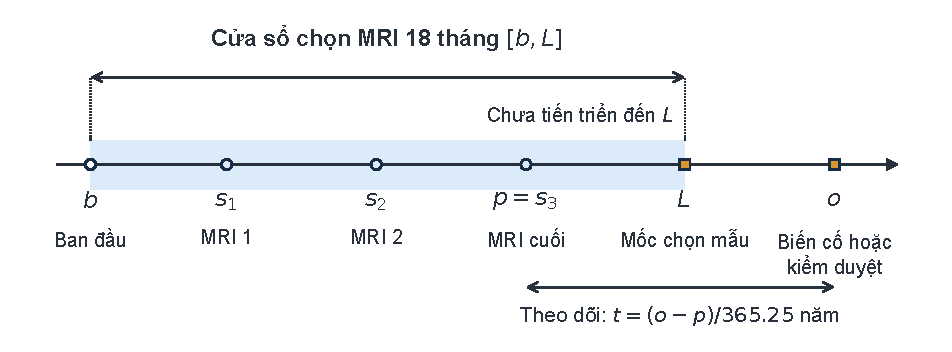
\includegraphics[width=\textwidth]{image/mci-progression-timeline.pdf}
\caption{Bài toán dự đoán tiến triển MCI theo thời gian}
\label{fig:problem-timeline}
\end{figure}

Hình~\ref{fig:problem-timeline} trực quan hóa tiến trình theo dõi và làm rõ mối quan hệ giữa ngày chụp MRI cuối cùng $p$ với mốc chọn mẫu $L$ (được ấn định bằng ngày khám ban đầu cộng 18 tháng lịch). Để lượng hóa trạng thái nhận thức và năng lực tự chủ của người bệnh, nghiên cứu sử dụng hai thang đo tiêu chuẩn:
\begin{enumerate}
\item \emph{MMSE (Mini-Mental State Examination)}: Thang điểm đánh giá nhận thức tổng quát từ 0 đến 30, trong đó điểm số càng thấp phản ánh mức độ sa sút nhận thức càng nghiêm trọng \cite{folstein1975mmse}.
\item \emph{CDR-global (Clinical Dementia Rating toàn cục)}: Các mức 0, 0.5, 1, 2 và 3 lần lượt tương ứng với bình thường, sa sút trí tuệ rất nhẹ, nhẹ, vừa và nặng theo bảng phân mức của đơn vị phát triển thang đo \cite{morris1993cdr,knightcdrscoring}.
\end{enumerate}

Theo tiêu chí nghiên cứu của Aghajanian và cộng sự \cite{aghajanian2025longitudinal}, khóa luận ghi nhận biến cố tiến triển ở lần khám đầu tiên sau mốc chọn mẫu $L$ có điểm MMSE $<24$ hoặc CDR-global $\geq1$. Đây là biến cố xác định bằng điểm số. Những người tham gia kết thúc theo dõi mà chưa từng ghi nhận biến cố được xem là \emph{kiểm duyệt phải} (right-censored) tại lần khám hợp lệ cuối cùng. Phân tích sống còn khai thác đồng thời cả thời gian theo dõi lẫn thông tin kiểm duyệt này.

Về mặt thiết kế phương pháp luận, khóa luận tính thời gian sống còn đến biến cố hoặc kiểm duyệt bắt đầu từ ngày chụp MRI cuối cùng $p$, trong khi tiêu chí chọn mẫu đòi hỏi người tham gia phải duy trì tình trạng chưa tiến triển cho đến mốc $L$. Chẳng hạn, với một người có lần MRI cuối ở tháng thứ 12 và mốc chọn mẫu ở tháng thứ 18, khoảng thời gian 6 tháng giữa $p$ và $L$ được tính vào thời gian theo dõi nhưng mặc nhiên không có biến cố. Do đó, đối tượng nghiên cứu được xác định chặt chẽ là nhóm bệnh nhân hồi cứu thỏa mãn điều kiện tại $L$. Khía cạnh phương pháp luận này, cùng nguy cơ sai lệch thời gian bất tử \cite{suissa2008immortal} khi diễn giải mô hình như một công cụ dự báo tại $p$, được trình bày và thảo luận cụ thể tại Mục~\ref{sec:study-design} và Mục~\ref{sec:study-limitations}.

\section{Thách thức và phạm vi nghiên cứu}
Việc xây dựng một mô hình học sâu sống còn trên dữ liệu y tế dọc đa phương thức đối mặt với ba thách thức phương pháp luận trung tâm:

Thứ nhất là \emph{đánh đổi giữa khả năng biểu diễn tương tác và số tham số cần ước lượng}. Phép ghép nối vectơ đặt các đặc trưng cạnh nhau để các tầng sau học mối liên hệ giữa chúng. Phép tích ngoài biểu diễn tường minh các tích chéo giữa các phương thức. Khi dùng một lớp tuyến tính đầy đủ để chiếu biểu diễn này, số trọng số tăng theo tích các kích thước đầu vào và đầu ra \cite{zadeh2017tensor,liu2018lowrank}. Với cỡ mẫu của khóa luận, đây là một nguy cơ quá khớp cần khảo sát. Phân rã CP giảm số trọng số bằng cách áp đặt cấu trúc hạng thấp \cite{kolda2009tensor,liu2018lowrank}. Ảnh hưởng của ràng buộc này đến năng lực phân biệt của mô hình cần được kiểm chứng bằng thực nghiệm.

Thứ hai là \emph{khả năng dư thừa thông tin giữa các nguồn dữ liệu}. Ảnh MRI và đặc trưng radiomics bắt nguồn từ cùng một thể tích ảnh gốc, còn các thang đo lâm sàng ở lần khám sau được dùng để xác định biến cố. Vì vậy, khóa luận kiểm tra bằng thực nghiệm liệu có cần giữ cả ba cặp tương tác hay chỉ cần hai cặp có chung đầu vào MRI. Hiệu quả dự báo của từng cấu hình được đánh giá qua so sánh loại bỏ thành phần.

Thứ ba là \emph{sự phức tạp của cấu trúc dữ liệu thời gian không đều và mục tiêu tối ưu hóa sống còn}. Mô hình phải xử lý đồng thời chuỗi quan sát có khoảng cách thời gian bất quy tắc bằng T-LSTM và attention, đồng thời tối ưu hóa hàm mất mát Cox trên các lô nhỏ mà không làm mất tính ổn định số học.

Để giải quyết thấu đáo ba thách thức trên, phạm vi nghiên cứu của khóa luận tập trung khảo sát có hệ thống: cách biểu diễn tương tác song tuyến qua tích ngoài, mức độ tinh giản tham số nhờ phân rã CP, và ảnh hưởng của việc lược bỏ cặp tương tác trong cấu trúc RC-Free. Mọi so sánh đối chứng đều được thực hiện nghiêm ngặt trên cùng một cách chia dữ liệu, sử dụng thống nhất ba mã khởi tạo ngẫu nhiên (seed) và đánh giá qua chỉ số đồng thuận (C-index), diện tích dưới đường cong ROC phụ thuộc thời gian (IPCW-ROC) cùng đường cong sống còn Kaplan--Meier.

\section{Câu hỏi nghiên cứu}
Nhằm định hướng cho toàn bộ các thực nghiệm đối chứng trong khóa luận, tôi xây dựng năm câu hỏi nghiên cứu cụ thể được tổng hợp tại Bảng~\ref{tab:rq}. Trong đó, RQ1 và RQ2 khảo sát vai trò của dữ liệu dọc và tính bổ khuyết của các nguồn dữ liệu đầu vào; RQ3 tập trung đối chiếu bản chất của phép hợp nhất tích ngoài so với ghép nối; trong khi RQ4 và RQ5 thẩm định hiệu quả giảm tham số của phân rã CP và tính ưu việt của cấu trúc tinh giản RC-Free.

\begin{table}[H]
\centering\small
\caption[Các câu hỏi nghiên cứu và phương pháp kiểm chứng]{Các câu hỏi nghiên cứu và phương pháp kiểm chứng.}
\label{tab:rq}
\setlength{\tabcolsep}{6pt}
\renewcommand{\arraystretch}{1.12}
\begin{tabularx}{\textwidth}{@{}Y Y@{}}
\toprule
\textbf{Câu hỏi nghiên cứu} & \textbf{Phương pháp kiểm chứng} \\
\midrule
\textbf{RQ1.} MRI ở nhiều thời điểm có mang lại khả năng phân biệt nguy cơ cao hơn so với chỉ dùng MRI cuối cùng không? & Đối chiếu mô hình \textit{MRI cuối} với \textit{MRI dọc và T-LSTM} cùng \textit{MRI dọc, T-LSTM và attention} để khảo sát vai trò của thông tin theo thời gian. \\
\addlinespace
\textbf{RQ2.} Bổ sung radiomics và lâm sàng có cải thiện khả năng phân biệt nguy cơ so với chỉ dùng MRI không? & Đối chiếu \textit{MRI dọc, T-LSTM và attention} với \textit{Ghép nối ba nguồn (thăm dò)} sử dụng cả ba nguồn dữ liệu. \\
\addlinespace
\textbf{RQ3.} Tương tác theo cặp có hiệu quả hơn ghép nối đặc trưng không? & So sánh ghép nối và tích ngoài qua ba lần chạy, dùng cùng cách huấn luyện và cùng trọng số ban đầu cho các phần chung. \\
\addlinespace
\textbf{RQ4.} CP giảm bao nhiêu tham số của lớp tương tác và ảnh hưởng thế nào đến C-index? & So sánh Full Outer-Product và Full CP Pairwise về C-index và số tham số ở từng phạm vi. \\
\addlinespace
\textbf{RQ5.} Có thể bỏ một số cặp tương tác và nhánh truyền mà vẫn duy trì khả năng phân biệt nguy cơ không? & Thực nghiệm loại bỏ thành phần đối chiếu 7 cấu trúc tương tác (gồm các biến thể 1 cặp, 2 cặp như RC-Free, MR-Free, MC-Free và Full CP) để đánh giá cấu trúc tối ưu. \\
\bottomrule
\end{tabularx}
\end{table}

\FloatBarrier
\Needspace{11\baselineskip}
\section{Đóng góp của khóa luận}
Khóa luận mang lại ba đóng góp phương pháp luận và thực nghiệm chính:
\begin{enumerate}
\item \emph{Xây dựng mô hình học sâu sống còn đa phương thức dọc toàn diện}: Đề xuất một kiến trúc hoàn chỉnh tích hợp đồng thời ba nguồn dữ liệu — ảnh MRI cấu trúc 3D, đặc trưng Radiomics định lượng và dữ liệu lâm sàng MMSE/CDR — qua ba mốc thăm khám dọc. Mô hình kết hợp bộ mã hóa ResNet-18 3D tiền huấn luyện trên dữ liệu y tế \cite{chen2019med3d}, mạng T-LSTM xử lý khoảng cách thời gian bất quy tắc \cite{baytas2017patient}, cơ chế attention học trọng số thăm khám then chốt và đầu ra nguy cơ Cox bán tham số.
\item \emph{Thiết kế cơ chế truyền phần dư có cổng và kiến trúc tinh gọn RC-Free}: Phát triển cơ chế kết nối phần dư có cổng điều tiết động (gated residual routing) giúp bảo toàn nguyên vẹn đường truyền gốc của từng phương thức, đồng thời xem thông tin tương tác như phần bổ chính có kiểm soát. Chọn MRI làm đầu vào chung cho hai cặp tương tác, tôi đề xuất cấu trúc \textbf{RC-Free} — lược bỏ cặp tương tác trực tiếp Radiomics--Lâm sàng (RC), tập trung tối đa vào hai tương tác cốt lõi xoay quanh MRI là MRI--Radiomics (MR) và MRI--Lâm sàng (MC).
\item \emph{Lượng hóa hiệu quả giảm tải tham số và năng lực phân tầng nguy cơ}: Thông qua phân rã tensor CP, mô hình cắt giảm tới \textbf{98.38\%} số tham số ở các lớp tương tác đầu và tiết kiệm \textbf{15460 tham số} toàn mạng khi loại bỏ cặp RC. Trên cùng một quy trình chia dữ liệu độc lập và đánh giá qua ba lần khởi tạo, RC-Free đạt C-index xác thực trung bình cao nhất trong bảy cấu trúc tương tác theo cặp (\textbf{0.8347}), phân tầng rõ nét hai nhóm nguy cơ trên đường cong Kaplan--Meier ($p=0.0134$ trên tập xác thực và $p<0.001$ trên tập kiểm tra hậu nghiệm), theo các kết quả của khóa luận ở Bảng~\ref{tab:interaction-parameters}, Bảng~\ref{tab:new-topology} và Bảng~\ref{tab:km-statistics}.
\end{enumerate}

\chapter[Cơ sở lý thuyết và nghiên cứu liên quan]{Cơ sở lý thuyết và\\nghiên cứu liên quan}
\label{chap:background}

\section{MCI, dữ liệu dọc và bài toán tiên lượng}
Chương trước đặt ra bài toán xếp hạng nguy cơ tiến triển từ MCI. Để giải quyết bài toán đó, trước hết cần mô tả được sự khác nhau về diễn biến giữa người bệnh. MCI có thể ổn định, cải thiện hoặc tiến triển \cite{petersen2018mci}; các khung đánh giá bệnh Alzheimer cũng phân biệt biểu hiện nhận thức với bằng chứng bệnh lý từ dấu ấn sinh học \cite{jack2018niaaa}.

Dữ liệu dọc cho phép quan sát cả trạng thái tại từng lần khám lẫn sự thay đổi giữa các lần khám. ADNI cung cấp MRI và các đánh giá nhận thức, lâm sàng theo thời gian \cite{weiner2015impact}. Đây là cơ sở để mô hình học diễn biến thay vì chỉ dựa vào một ảnh chụp.

\section{Phân tích sống còn và mô hình thời gian}
\subsection{Biến cố, kiểm duyệt và Cox}
Do thời gian theo dõi mỗi người khác nhau, phân tích sống còn nghiên cứu thời gian đến biến cố; trong bài toán này, biến cố là đạt ngưỡng tiến triển nhận thức. Chẳng hạn, một người kết thúc theo dõi mà chưa có biến cố được ghi $\delta_i=0$: ta biết thời gian chưa tiến triển ít nhất dài bằng thời gian đã quan sát, nhưng chưa biết biến cố sẽ xảy ra khi nào. Mô hình Cox biểu diễn nguy cơ tức thời, với điều kiện chưa có biến cố trước $t$, bằng \cite{cox1972regression}
\begin{equation}
 h_i(t)=h_0(t)\exp(\eta_i).
\end{equation}
Mô hình gồm hai thành phần: điểm nguy cơ $\eta_i$ do mạng học được và hàm nguy cơ nền $h_0(t)$. Trong đó, $\eta_i$ cho biết người nào có xu hướng tiến triển sớm hơn, còn $h_0(t)$ mô tả nguy cơ tại từng thời điểm khi $\eta=0$. DeepSurv dùng mạng nơ-ron để học điểm nguy cơ phi tuyến trong cấu trúc Cox này \cite{katzman2018deepsurv}.

Tuy nhiên, điểm nguy cơ $\eta_i$ phản ánh nguy cơ tương đối giữa các cá thể, chưa cho biết xác suất tiến triển tuyệt đối tại một thời hạn cụ thể, chẳng hạn sau 3 năm. Muốn tính xác suất đó, cần ước lượng thêm nguy cơ tích lũy nền $H_0(t)$ từ thời gian theo dõi, biến cố và điểm nguy cơ trên tập huấn luyện. Sau đó, cần kiểm tra độ hiệu chỉnh, tức xem xác suất dự đoán có phù hợp với tỷ lệ biến cố quan sát hay không.

Khi thời điểm biến cố không trùng nhau, đối của log-hợp lý riêng phần là
\begin{equation}
\mathcal L_{\rm Cox}=-\sum_{i:\delta_i=1}\left[\eta_i-\log\sum_{j\in\mathcal R(t_i)}\exp(\eta_j)\right],
\end{equation}
trong đó $\mathcal R(t_i)$ gồm người còn được theo dõi và chưa có biến cố trước $t_i$. Breslow xử lý biến cố trùng thời gian \cite{breslow1974covariance}; C-index đánh giá thứ tự nguy cơ trên các cặp so sánh được \cite{harrell1996multivariable}.

Bên cạnh mô hình nguy cơ, phân tích sống còn cần một mốc bắt đầu theo dõi rõ ràng. Phương pháp dự đoán tại mốc xác định (landmarking) chọn người đủ điều kiện tại một thời điểm, rồi theo dõi biến cố từ thời điểm đó \cite{vanhouwelingen2007dynamic}. Mục~\ref{sec:study-design} trình bày hai mốc được dùng trong bộ dữ liệu của khóa luận.


\begin{figure}[H]
\centering
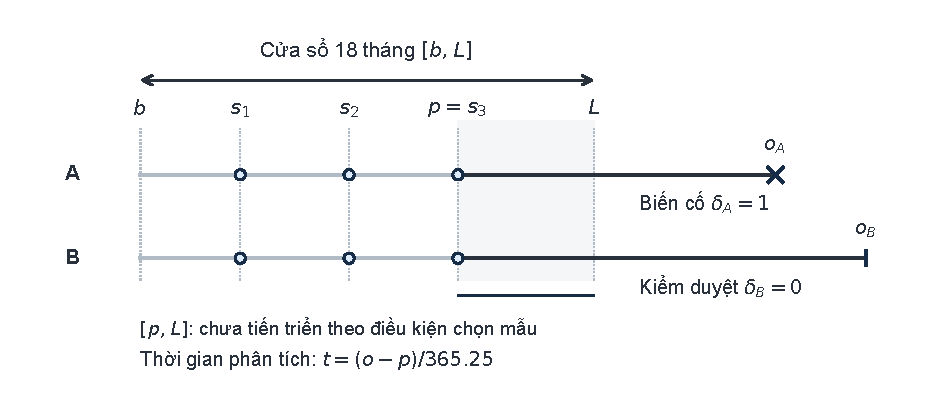
\includegraphics[width=\textwidth]{image/concept-survival.pdf}
\caption[Biến cố và kiểm duyệt phải]{Minh họa biến cố và kiểm duyệt: dấu nhân chỉ biến cố; vạch đứng chỉ thời điểm kết thúc theo dõi khi chưa ghi nhận biến cố.}
\label{fig:concept-survival}
\end{figure}

\subsection{T-LSTM và attention}
Để đưa lịch sử khám vào mô hình sống còn, LSTM tổng hợp chuỗi qua trạng thái ẩn, bộ nhớ và các cổng điều tiết \cite{hochreiter1997lstm}. Do khoảng cách giữa các lần khám không đều, T-LSTM bổ sung khoảng thời gian này vào phép điều chỉnh bộ nhớ \cite{baytas2017patient}. Sau đó, additive attention kết hợp các trạng thái bằng trọng số học được \cite{bahdanau2015attention}:
\begin{equation}
 e_t=\bm v^\top\tanh(W_hh_t+b_h),\quad
 \alpha_t=\frac{\exp(e_t)}{\sum_k\exp(e_k)},\quad z=\sum_t\alpha_th_t.
\end{equation}
Ở đây, $\alpha_t$ là trọng số mà mạng gán cho trạng thái tại lần khám $t$ khi tạo biểu diễn chung. Cấu hình T-LSTM và cách xử lý thời gian của mô hình cuối được trình bày ở Chương~\ref{chap:method}.

Có thể đọc Hình~\ref{fig:concept-longitudinal} theo hai bước: T-LSTM cập nhật thông tin từ các lần khám trước và xét khoảng cách thời gian; attention xác định mức đóng góp của từng trạng thái ẩn vào biểu diễn chung.

\begin{figure}[H]
\centering
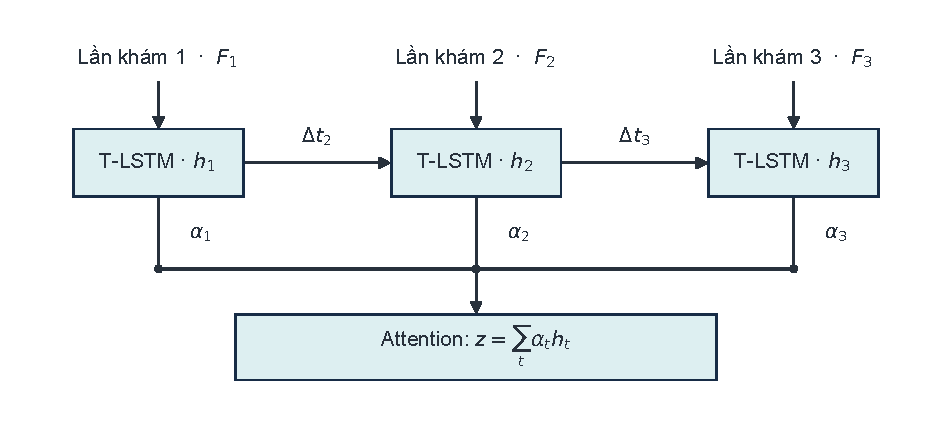
\includegraphics[width=\textwidth]{image/concept-longitudinal.pdf}
\caption[Tổng hợp thông tin qua các lần khám]{Sơ đồ khái niệm về dữ liệu dọc: khoảng thời gian giữa các lần khám và trọng số attention có vai trò khác nhau. Chi tiết phép cập nhật T-LSTM nằm ở Chương 3.}
\label{fig:concept-longitudinal}
\end{figure}

\section{Ba nguồn thông tin và biểu diễn}
\begin{table}[H]
\centering\small
\caption[Ba nguồn thông tin trong bài toán]{Thông tin chính của ba nguồn dữ liệu.}
\label{tab:background-inputs}
\begin{tabularx}{\linewidth}{@{}L{2.4cm}Y Y@{}}
\toprule
\textbf{Nguồn} & \textbf{Thông tin chính} & \textbf{Điểm cần lưu ý} \\
\midrule
MRI cấu trúc & Hình thái não; CNN học biểu diễn không gian & Cần chuẩn hóa và kiểm tra khác biệt miền ảnh \\
Radiomics & Phép đo hình dạng, cường độ và kết cấu & Phụ thuộc vùng não, chuẩn hóa và rời rạc hóa; có thể trùng thông tin MRI \\
Lâm sàng & MMSE, CDR và khả năng sinh hoạt & Liên quan tiêu chí biến cố; cần phân biệt thời điểm đo đầu vào với kết cục \\
\bottomrule
\end{tabularx}
\end{table}

Với nguồn ảnh, CNN 3D học quan hệ giữa các voxel trong thể tích. ResNet dùng kết nối residual để học phần hiệu chỉnh trên đầu vào \cite{he2016deep}; Med3D/MedicalNet cung cấp trọng số tiền huấn luyện ảnh y tế 3D \cite{chen2019med3d}. Khóa luận dùng ResNet-18 3D khởi tạo từ MedicalNet làm bộ mã hóa MRI chung cho các đối chứng chính. Li và cộng sự cũng cho thấy biểu diễn MRI có thể hỗ trợ tiên lượng, nhưng dùng hồi hải mã tại một thời điểm và đánh giá trên ADNI/AIBL, khác chuỗi MRI toàn não ở đây \cite{li2019hippocampal}.

Khác với đặc trưng học trực tiếp từ ảnh, radiomics biến MRI thành các phép đo định trước \cite{vangriethuysen2017computational}. Vì nhiều đặc trưng tương quan, PCA tạo các tổ hợp tuyến tính theo hướng phương sai lớn để giảm chiều \cite{jolliffe2016pca}. Các tham số PCA được học trên tập huấn luyện theo phương sai của đặc trưng; giá trị tiên lượng của biểu diễn sau giảm chiều được đánh giá bằng mô hình sống còn.

Để bổ sung thông tin chức năng, MMSE và CDR phản ánh nhận thức và chức năng sinh hoạt \cite{folstein1975mmse,morris1993cdr}. Các số đo ở lần khám đầu vào khác vai trò với đánh giá sau $L$ dùng tạo nhãn. Khi dữ liệu thiếu, chỉ báo quan sát giúp phân biệt giá trị đo thật với giá trị được điền; các biến và chỉ báo cụ thể được mô tả ở Mục~\ref{sec:preprocessing}.


\begin{figure}[H]
\centering
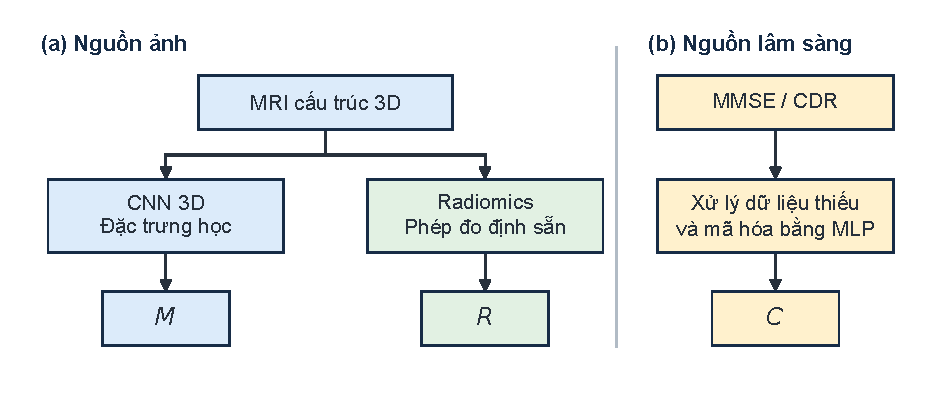
\includegraphics[width=\textwidth]{image/concept-sources.pdf}
\caption[Nguồn gốc của ba biểu diễn]{MRI và radiomics cùng xuất phát từ ảnh, nhưng cách tạo đặc trưng khác nhau. Dữ liệu lâm sàng bổ sung các đánh giá nhận thức và chức năng.}
\label{fig:concept-sources}
\end{figure}

\section{Hợp nhất thông tin và tham số hóa tương tác}
Để kết hợp các nguồn trên, mô hình cần đưa các biểu diễn về kích thước phù hợp \cite{baltrusaitis2019multimodal}. Có hai cách cơ bản: ghép nối giữ các vectơ cạnh nhau, còn tích ngoài tạo tường minh mọi tích chéo giữa hai vectơ \cite{zadeh2017tensor}. CP làm gọn trọng số dùng để xử lý các tích chéo này. Sau đó, cổng phần dư quyết định bổ sung bao nhiêu thông tin tương tác vào mỗi nguồn.


Hình~\ref{fig:concept-fusion} dùng hai vectơ hai chiều để phân biệt hai phép toán. Ghép nối chỉ xếp các tọa độ cạnh nhau; tích ngoài tạo thêm các tích giữa mọi cặp tọa độ. Lớp học sau đó mới chuyển những giá trị này thành đặc trưng phục vụ dự báo.

\begin{figure}[H]
\centering
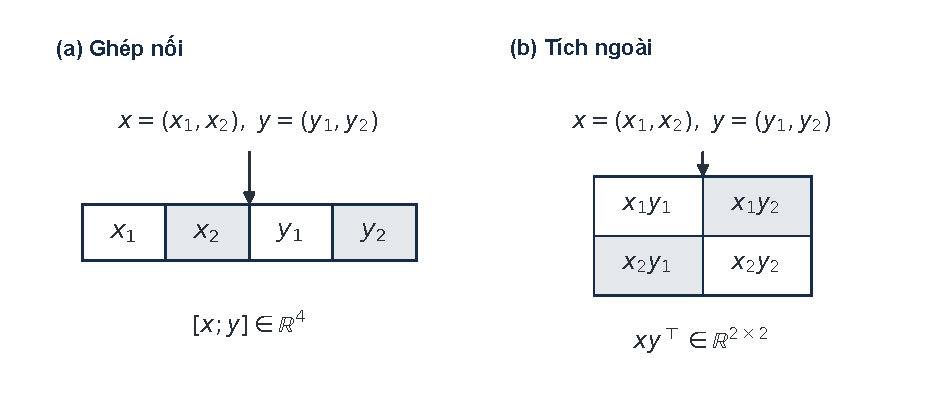
\includegraphics[width=\textwidth]{image/concept-fusion.pdf}
\caption[Ghép nối và tích ngoài qua ví dụ ký hiệu]{Ghép nối và tích ngoài của hai vectơ hai chiều.}
\label{fig:concept-fusion}
\end{figure}

\subsection{Từ tích ngoài đến CP}
Tích ngoài tạo các tương tác giữa mọi cặp đặc trưng của hai nguồn. Số tổ hợp tăng theo tích số chiều, khiến số trọng số cần học tăng nhanh. CP (CANDECOMP/PARAFAC, phân rã tensor thành tổng các thành phần hạng một) giúp thu gọn trọng số bằng các nhân tử hạng thấp. Hình~\ref{fig:cp-intro} minh họa hai cách tính; Chương~\ref{chap:method} trình bày ứng dụng cụ thể.
\begin{figure}[H]
\centering
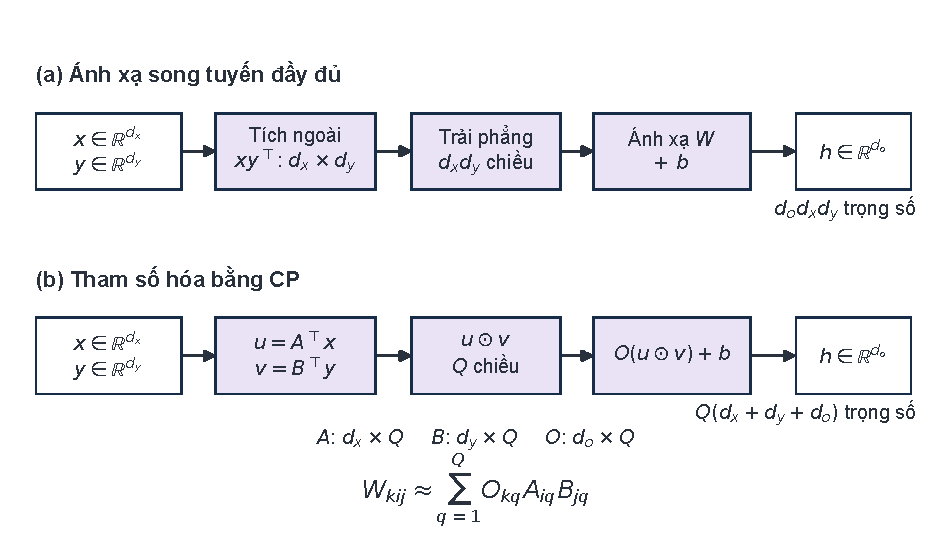
\includegraphics[width=\textwidth]{image/cp-concept-general.pdf}
\caption[Minh họa tích ngoài và CP]{Hai cách tính ánh xạ song tuyến với kích thước tổng quát: tích ngoài và tham số hóa CP hạng $Q$. Số trọng số trong hình chưa gồm hệ số chệch $b$.}
\label{fig:cp-intro}
\end{figure}
Với hai vector cột $x\in\mathbb R^{d_x\times1}$ và $y\in\mathbb R^{d_y\times1}$, tích ngoài $xy^\top\in\mathbb R^{d_x\times d_y}$ chứa mọi tích $x_iy_j$. Trải ma trận rồi áp dụng ánh xạ tuyến tính tương đương ánh xạ song tuyến:
\begin{equation}
 h_k=\sum_{i=1}^{d_x}\sum_{j=1}^{d_y}W_{kij}x_iy_j+b_k.
\end{equation}
Tensor trọng số $W\in\mathbb R^{d_o\times d_x\times d_y}$ có $d_od_xd_y$ phần tử. CP biểu diễn tensor bằng tổng các thành phần hạng một \cite{carroll1970candecomp,kolda2009tensor}:
\begin{equation}
 W_{kij}\approx\sum_{q=1}^Q O_{kq}A_{iq}B_{jq},\qquad
 h=O[(A^\top x)\odot(B^\top y)]+b.
\end{equation}
Số trọng số còn $Q(d_x+d_y+d_o)$, đổi lại giới hạn năng lực biểu diễn. Các nhân tử $A$, $B$ và $O$ được học trực tiếp trong mạng. Low-rank Multimodal Fusion (LMF, hợp nhất đa nguồn hạng thấp) dùng nhân tử hạng thấp cho hợp nhất \cite{liu2018lowrank}, còn Multimodal Tucker Fusion (MUTAN) dùng phân rã Tucker, trong đó tensor lõi kết hợp các nhân tử theo từng chiều \cite{benyounes2017mutan}; chúng cung cấp cơ sở cho việc khảo sát tham số hóa tương tác trong khóa luận.

\subsection{Gated residual}
Sau khi tạo tương tác, mô hình cần quyết định đưa bao nhiêu thông tin đó trở lại từng nguồn. Kết nối phần dư giữ đường biểu diễn gốc và cộng một phần bổ sung; cổng học từ đầu vào điều tiết phần bổ sung theo từng mẫu. Hai nghiên cứu dưới đây cung cấp cơ sở cho cách tổ chức này.

\paragraph{Ryumina và cộng sự: lấy văn bản làm nguồn neo.}
Text Residual Fusion kết hợp văn bản, âm thanh, khuôn mặt và cảnh để nhận dạng sự lưỡng lự \cite{ryumina2026residual}. Sau phép chiếu riêng, đặt $b=h_{\rm text}$ và $h_m$ là biểu diễn nguồn còn lại. Công thức (13) của bài báo có dạng
\begin{equation}
 g_m=\sigma(\operatorname{MLP}([b;h_m])),\qquad
 z=\operatorname{LN}\left(b+\sum_{m\ne\mathrm{text}}g_m d_m(h_m)\right).
 \label{eq:ryumina-residual}
\end{equation}
Ở đây, $[b;h_m]$ là ghép nối, $\sigma$ là sigmoid và $d_m$ là MLP tạo phần dư. Cổng xét đồng thời nguồn neo và nguồn bổ sung; tổng các phần dư được cộng vào văn bản rồi chuẩn hóa. Đặc trưng hợp nhất đi qua bộ phân loại. Hình~\ref{fig:literature-gates}(a) tóm tắt luồng này.

\paragraph{Liu và cộng sự: bổ sung chuyển động vào RGB.}
DyFADet+ dùng hai nhánh RGB và bộ xương, tạo các mức đặc trưng thời gian tương ứng để phát hiện cử chỉ \cite{liu2026motion}. Tại mức $\ell$, công thức (1)--(2) của bài báo là
\begin{align}
 G^{(\ell)}&=\sigma\left(\phi_\ell([F_r^{(\ell)};F_s^{(\ell)}])\right),\\
 F_f^{(\ell)}&=F_r^{(\ell)}+\alpha G^{(\ell)}\odot\psi_\ell(F_s^{(\ell)}).
 \label{eq:liu-residual}
\end{align}
$F_r$ và $F_s$ lần lượt biểu diễn RGB và bộ xương; $\phi_\ell$ là tích chập thời gian $1\times1$, còn $\psi_\ell$ là bộ chuyển đổi hai lớp tích chập với GELU. Cổng chọn mức bổ sung theo phần tử, còn $\alpha=0.5$ điều chỉnh cường độ chung. Các đặc trưng hợp nhất được đưa tới đầu phát hiện theo thời gian, như Hình~\ref{fig:literature-gates}(b).

\begin{figure}[H]
\centering
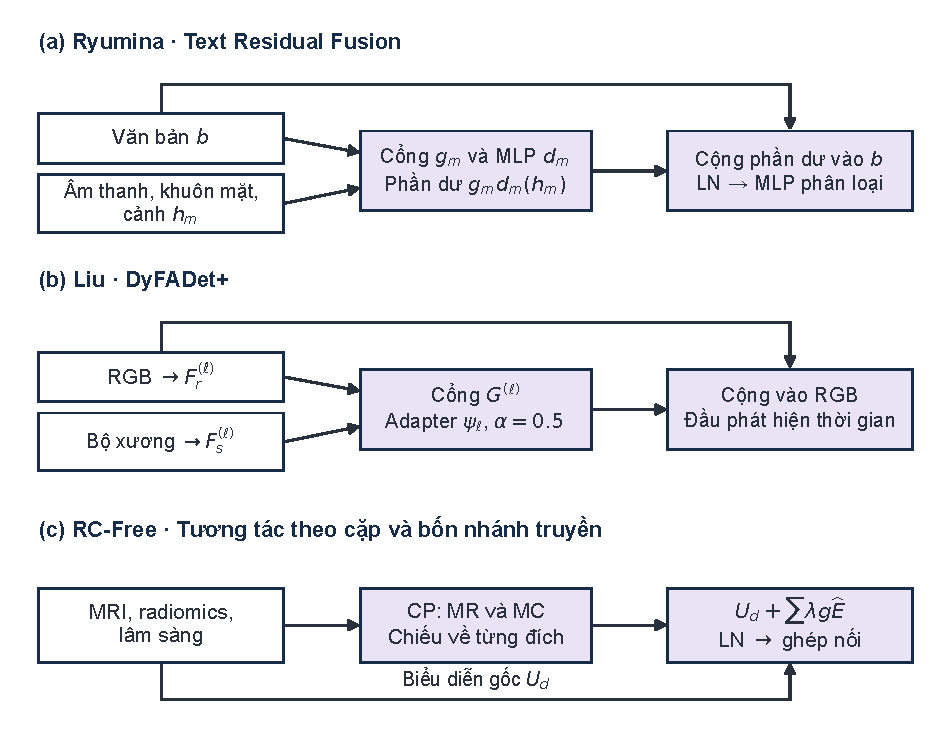
\includegraphics[width=\textwidth]{image/literature-gates.pdf}
\caption[Hai phương pháp phần dư có cổng và hướng thích nghi]{Sơ đồ khái quát được vẽ lại từ Ryumina và cộng sự \cite{ryumina2026residual} và Liu và cộng sự \cite{liu2026motion}. Các ô chỉ thể hiện luồng chính; dòng (c) là thiết kế của khóa luận.}
\label{fig:literature-gates}
\end{figure}

\paragraph{Từ hai ý tưởng trên đến thiết kế của khóa luận.}
Cơ sở thiết kế gồm ba bước. Thứ nhất, giữ biểu diễn gốc $U_d$ của từng nguồn để thông tin riêng vẫn có đường đi trực tiếp. Thứ hai, thay phần bổ sung từ một nguồn bằng đặc trưng tương tác CP của một cặp; phép chiếu riêng đưa tương tác về đúng số chiều của nguồn đích, tạo $\widehat E_{k\to d}$. Thứ ba, dùng cổng xét cả nguồn đích và phần bổ sung, rồi cộng các nhánh cùng đích:
\begin{equation}
 Z_d=\operatorname{LN}\left[U_d+\sum_{k\in\mathcal P(d)}\lambda_{k\to d}g_{k\to d}\widehat E_{k\to d}\right].
\end{equation}
Đây là lựa chọn kiến trúc dựa trên nguyên tắc phần dư có điều tiết. Trong RC-Free, MR (MRI--radiomics) truyền về MRI và radiomics; MC (MRI--lâm sàng) truyền về MRI và lâm sàng. Vì vậy, cả ba nguồn đều có đường gốc và bốn nhánh bổ sung được học riêng.

Hai hệ số đảm nhiệm hai vai trò khác nhau. $g_{k\to d}\in(0,1)$ là một số thay đổi theo người và lần khám, do MLP với sigmoid tạo ra. $\lambda_{k\to d}$ là tham số dùng chung của nhánh, khởi tạo bằng 0.1 và được học không ràng buộc dấu. Chẳng hạn, khi $\lambda=0.1$ và $g=0.2$, phần bổ sung trước phép cộng là $0.02\widehat E$; nếu $g=0.8$ thì thành $0.08\widehat E$. Như vậy, $\lambda$ đặt mức điều chỉnh chung, còn $g$ thay đổi mức tiếp nhận theo đầu vào. Khi $\lambda$ âm, hướng bổ sung đảo lại. LayerNorm chuẩn hóa tổng sau phép cộng; Mục~\ref{sec:gated-routing} trình bày đầy đủ phép chiếu và MLP của cổng.

\section{Nghiên cứu liên quan và hướng khảo sát}
\label{sec:related-work}
\begin{table}[H]
\centering\small
\caption[Tổng hợp nghiên cứu liên quan]{Các hướng nghiên cứu, phương pháp và thành phần được kế thừa.}
\label{tab:related}
\begin{tabularx}{\linewidth}{@{}L{3cm}Y Y@{}}
\toprule
\textbf{Hướng} & \textbf{Công trình và cách làm} & \textbf{Liên hệ với khóa luận} \\
\midrule
MRI đơn thời điểm & Li: biểu diễn hồi hải mã; Nakagawa: thể tích chất xám và mạng sống còn \cite{li2019hippocampal,nakagawa2020survival} & Cơ sở khảo sát biểu diễn ảnh và mục tiêu sống còn \\
Dữ liệu dọc & Li--Fan, Ding: nhận thức/MRI theo thời gian; Dong: học thay đổi từ cặp MRI \cite{li2019early,ding2023progression,dong2021deepatrophy} & Phân biệt học diễn biến với dự đoán biến cố tương lai \\
Radiomics và lâm sàng & Tang: LASSO--Cox, kết hợp thêm biến lâm sàng/xét nghiệm \cite{tang2021individualized} & Kiểm tra thông tin bổ sung trong cùng thiết lập \\
MRI dọc học sâu & Aghajanian: CNN--PCA--T-LSTM và attention \cite{aghajanian2025longitudinal} & Quy trình tham chiếu và cách đánh giá phân tầng nguy cơ \\
\bottomrule
\end{tabularx}
\end{table}

Trong các công trình ở Bảng~\ref{tab:related}, Aghajanian và cộng sự là tham chiếu gần nhất: 228 người MCI có ba MRI trong 18 tháng. CNN được huấn luyện trước, sau đó trích vector 512 chiều, dùng PCA giữ 99\% phương sai và đưa vào T-LSTM với attention \cite{aghajanian2025longitudinal}. Bài báo đánh giá điểm nguy cơ bằng C-index, KM và ROC tại các thời hạn. Radiomics chất xám chưa đem lại cải thiện nhất quán; mô hình cuối không giữ nguồn này. Kết quả này gợi mở việc khảo sát cách kết hợp biểu diễn ảnh với các nguồn bổ sung.

Từ quy trình này, bản \emph{Baseline Reproduction (CNN--PCA--T-LSTM)} của khóa luận kế thừa quy trình trên nhưng dùng 359 người, tiền xử lý và cấu hình khác. Đây là bản tái lập có điều chỉnh. RC-Free còn thay đổi cách hợp nhất và cấu hình huấn luyện, nên chênh lệch giữa hai quy trình không thể quy riêng cho CP hay cổng.

\subsection{Từ bằng chứng trước đến thiết kế nghiên cứu}
\label{sec:research-gaps}
Dữ liệu dọc có thể mô tả thay đổi, nhưng lợi ích tiên lượng cần được kiểm chứng thay vì mặc định tốt hơn ảnh đơn thời điểm. Tương tự, MRI và radiomics cùng nguồn ảnh nên có thể bổ sung hoặc lặp thông tin; biến lâm sàng còn liên quan trực tiếp tiêu chí kết cục. Vì vậy, các đối chứng đầu vào đóng vai trò thăm dò, còn trọng tâm là kiểm tra cách hợp nhất trong điều kiện so sánh rõ ràng.

Tương tác tường minh làm số tham số tăng theo tích số chiều. Khóa luận đối chiếu ghép nối với tích ngoài, rồi dùng CP để kiểm tra đánh đổi giữa kích thước lõi tương tác và C-index. Nghiên cứu cũng kiểm tra việc chỉ giữ MR (MRI--radiomics) và MC (MRI--lâm sàng). Kết quả nhiều lần khởi tạo và phân tích sống còn của RC-Free giúp mô tả khả năng phân biệt/phân tầng nguy cơ.

Như vậy, các nghiên cứu trước cung cấp từng thành phần nhưng chưa quyết định cách hợp nhất phù hợp cho nhóm dữ liệu hiện tại. Chương~\ref{chap:method} cụ thể hóa lựa chọn này thành quy trình dữ liệu, mô hình RC-Free và cách đánh giá.

\chapter{Phương pháp}
\label{chap:method}

\section{Tổng quan mô hình RC-Free}
\label{sec:final-pipeline}
Hình~\ref{fig:overall} trình bày bốn khối của mô hình RC-Free. Tại mỗi lần khám, ba bộ mã hóa tạo biểu diễn cho ảnh MRI ($M$), đặc trưng radiomics ($R$) và dữ liệu lâm sàng ($C$). Từ ba biểu diễn này, khối RC-Free tính hai tương tác MRI--radiomics (MR) và MRI--lâm sàng (MC), rồi đưa thông tin từ mỗi tương tác trở về hai biểu diễn thành phần qua tổng cộng bốn nhánh có cổng. Mỗi bộ mã hóa và khối hợp nhất dùng chung trọng số qua cả ba lần khám. T-LSTM xử lý chuỗi đặc trưng đã hợp nhất, sau đó cơ chế attention tổng hợp các trạng thái ẩn thành một vectơ để khối Cox tính điểm nguy cơ.

\begin{figure}[H]
\centering
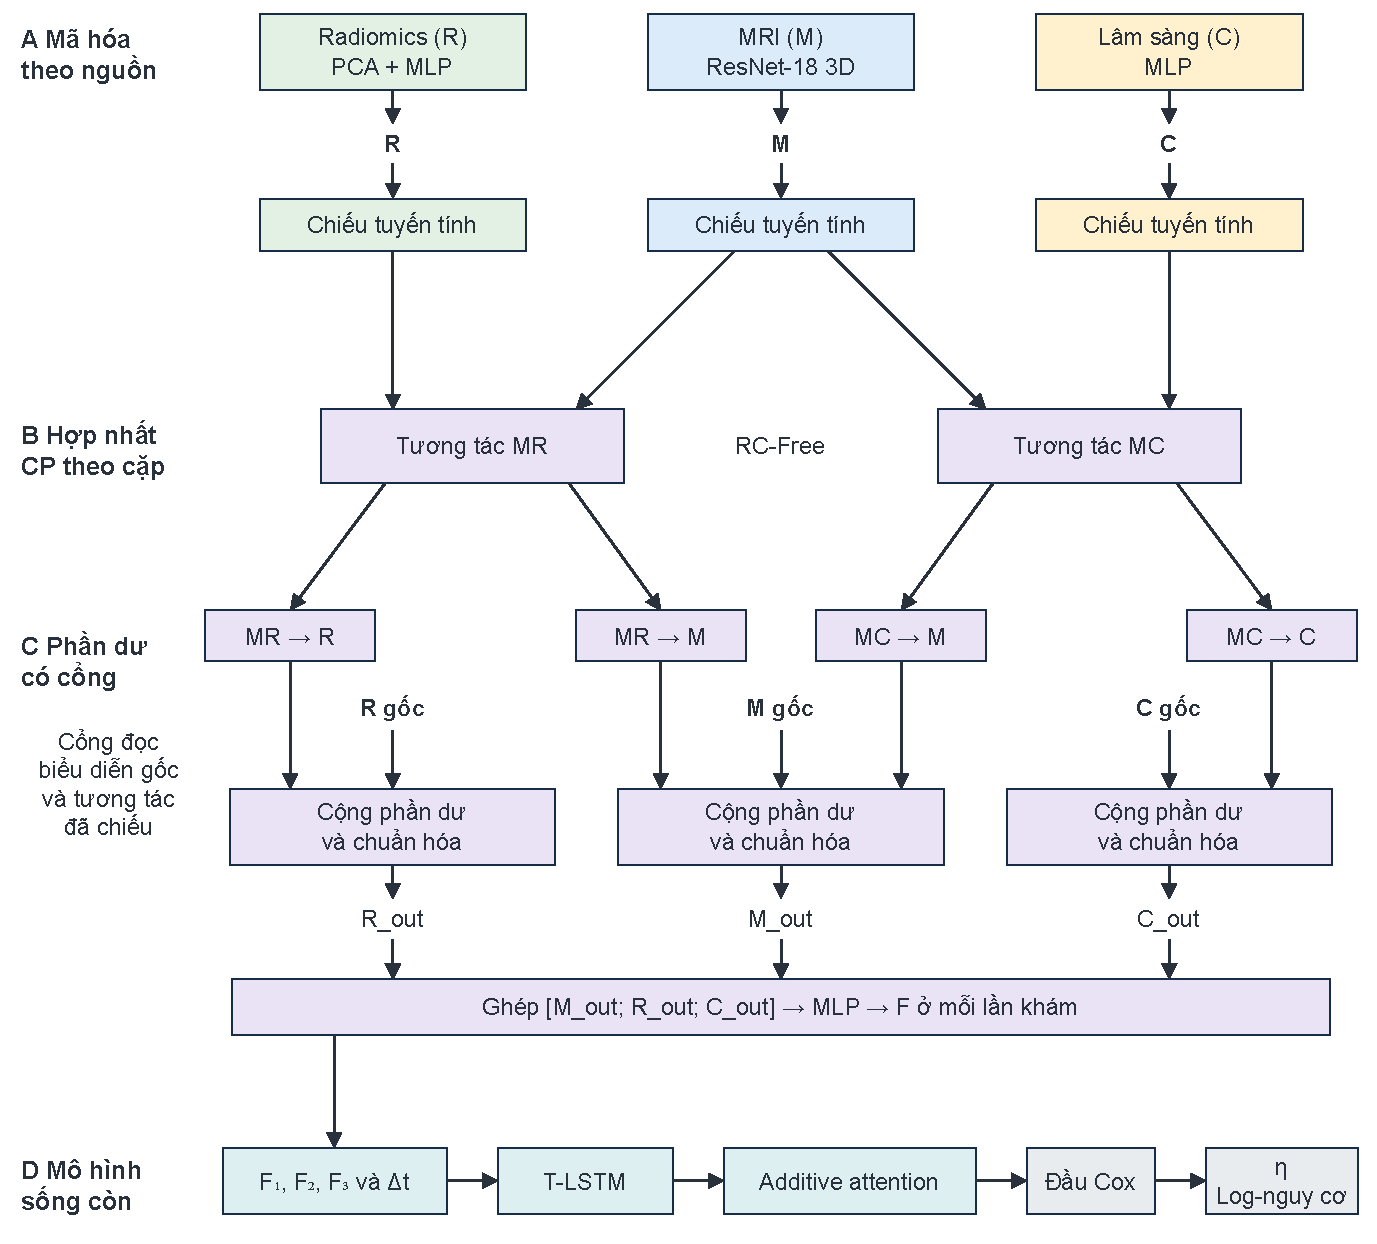
\includegraphics[width=\textwidth]{image/final-pipeline.pdf}
\caption{Sơ đồ quy trình xử lý tổng thể của mô hình RC-Free}
\label{fig:overall}
\end{figure}
\FloatBarrier

Sơ đồ tổng hợp từ dữ liệu dọc đến đánh giá sống còn được trình bày ở Hình~\ref{fig:master-pipeline}, Phụ lục~\ref{app:master-pipeline}.

\section{Thiết kế nghiên cứu và xây dựng dữ liệu}
\label{sec:study-design}

\subsection{Tiêu chí chọn mẫu và ba lần khám}
Dữ liệu nghiên cứu lấy từ Alzheimer's Disease Neuroimaging Initiative (ADNI), một nghiên cứu dọc đa trung tâm về suy giảm nhận thức và AD \cite{weiner2015impact,jack2008adnimri}. Sau khi liên kết mã người tham gia dạng chuỗi (PTID) với mã số người tham gia (RID) trong ADNI, tôi chọn cho mỗi người lần khám ban đầu sớm nhất thuộc ADNI1, ADNIGO hoặc ADNI2 thỏa mãn đồng thời ba điều kiện: có ngày hợp lệ, có mã lần khám \texttt{bl} và có chẩn đoán MCI (mã 2). Ký hiệu $b_i$ là ngày khám ban đầu của người $i$ và $L_i=b_i+18$ tháng lịch là \emph{mốc xét điều kiện chọn mẫu}.

Để giữ nhóm chưa tiến triển trong giai đoạn quan sát, người tham gia bị loại nếu có chẩn đoán AD trong bảng tổng hợp chẩn đoán DXSUM, MMSE $<24$ hoặc CDR-global $\geq1$ tại hoặc trước $L_i$. Sau $L_i$, cần ít nhất một đánh giá MMSE hoặc CDR hợp lệ để xác định biến cố hoặc kiểm duyệt.

Với mỗi người đủ điều kiện, ba ảnh MRI được chọn trong khoảng $[b_i,L_i]$. Việc xếp nhóm bắt đầu từ lần chụp sớm nhất chưa thuộc nhóm nào và gộp vào cùng nhóm các lần chụp tiếp theo trong vòng hai tháng lịch kể từ ngày đó. Trong mỗi nhóm, ảnh chụp chính được ưu tiên hơn ảnh chụp lặp, sau đó mới xét thứ tự hiệu chỉnh ghi trong mô tả ảnh ADNI. Nếu nhiều ảnh cùng mức ưu tiên, ảnh có mã nhỏ nhất được chọn. Khi có hơn ba nhóm, tôi giữ ảnh đầu, ảnh cuối và ảnh trung gian có ngày chụp gần trung điểm thời gian giữa hai ảnh này nhất. Ba ngày chụp thỏa mãn $s_{i1}<s_{i2}<s_{i3}\leq L_i$.

Bảng kiểm soát chất lượng chính thức chưa được liên kết với mã ảnh, nên quy trình dùng nhãn xử lý để xếp thứ tự ưu tiên. Với ADNI1, thứ tự là N3+Scaled+GradWarp+B1, N3+Scaled+GradWarp, N3+Scaled, N3+GradWarp+B1, N3+GradWarp và N3. Với ADNIGO và ADNI2, thứ tự là N3m+GradWarp, N3m, N3+GradWarp và N3. Ảnh không khớp các nhãn trên được xếp sau. B1 biểu thị hiệu chỉnh độ lệch trường tần số vô tuyến, GradWarp biểu thị hiệu chỉnh méo hình học do cuộn chênh từ, N3 và N3m biểu thị hiệu chỉnh bất đồng nhất cường độ, còn Scaled biểu thị chuẩn hóa kích thước theo mẫu đo (phantom).\footnote{Mô tả hiệu chỉnh ảnh của ADNI: \url{https://adni.loni.usc.edu/data-samples/adni-data/neuroimaging/mri/mri-pre-processing/}.} Bảng kê lưu mã ảnh đã chọn cùng thứ tự ưu tiên để có thể truy vết từng lựa chọn.



Hình~\ref{fig:cohort} tóm tắt quá trình lọc từ 899 người có MRI và liên kết định danh thành công xuống 359 người, mỗi người đúng ba MRI, tổng cộng 1077 ảnh. Trong 359 người được chọn, 106 người có biến cố và 253 người bị kiểm duyệt. Xét theo giai đoạn tuyển vào nghiên cứu, 78 người thuộc ADNI1, 80 người thuộc ADNIGO và 201 người thuộc ADNI2.

\begin{figure}[H]
\centering
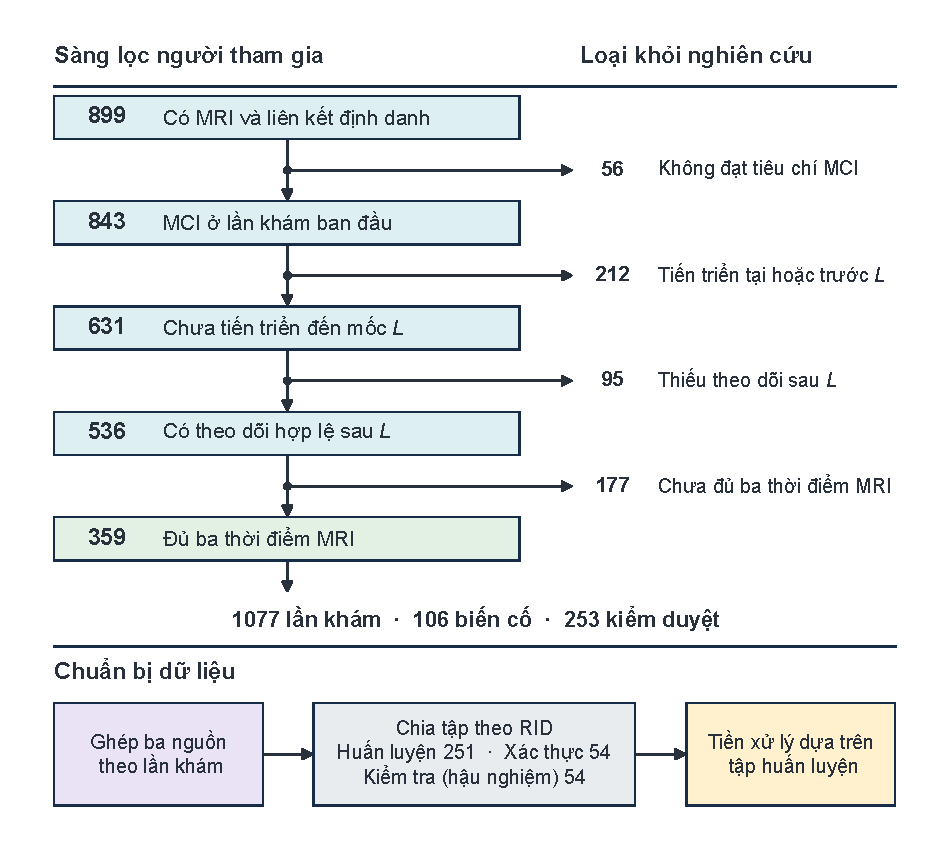
\includegraphics[width=\textwidth]{image/cohort-construction.pdf}
\caption{Quy trình xây dựng và chọn lọc nhóm nghiên cứu dọc}
\label{fig:cohort}
\end{figure}

\subsection{Biến cố, kiểm duyệt và mốc tính thời gian}
Sau mốc chọn mẫu $L_i$, lần đánh giá hợp lệ đầu tiên có MMSE $<24$ hoặc CDR-global $\geq1$ được lấy làm thời điểm ghi nhận biến cố tiến triển. Nếu chưa ghi nhận biến cố, người tham gia được kiểm duyệt tại lần đánh giá MMSE hoặc CDR hợp lệ cuối cùng. Các giá trị thiếu hoặc không hợp lệ không được tính là biến cố.

\Needspace{8\baselineskip}
Thời gian sống còn $t_i$ được tính bằng năm, từ ngày chụp MRI cuối trong ba lần đã chọn ($p_i=s_{i3}$) đến ngày ghi nhận biến cố hoặc kiểm duyệt ($o_i$). Cùng với khoảng thời gian này, chỉ báo $\delta_i$ xác định người tham gia có biến cố (bằng 1) hay bị kiểm duyệt (bằng 0). Hai thành phần của nhãn được tính như sau:
\begin{equation}
 t_i=\frac{o_i-p_i}{365.25},\qquad
 \delta_i=\begin{cases}1,&\text{có biến cố},\\0,&\text{bị kiểm duyệt}.\end{cases}
 \label{eq:survival-target}
\end{equation}

Mốc $L_i$ xác định điều kiện chọn mẫu, còn ngày MRI cuối $p_i$ là gốc tính thời gian sống còn. Trong 359 người, 356 người chụp MRI cuối trước $L_i$ và ba người chụp đúng mốc này. Khoảng cách $L_i-p_i$ có trung vị 186 ngày, khoảng tứ phân vị 169--197 ngày và phạm vi 0--288 ngày. Với những người có $p_i<L_i$, điều kiện chưa tiến triển đến $L_i$ bảo đảm họ không có biến cố trong khoảng từ $p_i$ đến $L_i$. Vì vậy, việc chọn những người này phụ thuộc vào thông tin thu thập sau ngày MRI cuối.

Nếu lấy $p_i$ làm thời điểm dự báo, khoảng theo dõi được bảo đảm không có biến cố có thể gây sai lệch thời gian bất tử (immortal time bias) \cite{suissa2008immortal}.

\subsection{Phân chia dữ liệu và hạn chế rò rỉ thông tin}
\label{sec:data-split}
Tôi chia dữ liệu cố định theo RID để mọi ảnh MRI của một người đều thuộc cùng một tập. Ba tập lần lượt gồm 251 người huấn luyện, 54 người xác thực và 54 người kiểm tra, với số biến cố tương ứng là 74, 16 và 16. Khi ghép các nguồn theo mã người, lần khám, mã ảnh và tập dữ liệu, mỗi lần khám phải có duy nhất một kết quả khớp giữa các nguồn. Chỉ dữ liệu huấn luyện được dùng để xác định cách điền dữ liệu thiếu, ước lượng tham số chuẩn hóa, nhận diện đặc trưng hằng và học PCA. Các biến dự báo không bao gồm chẩn đoán, trạng thái biến cố, ngày kết cục và thời gian sống còn.

Mỗi ảnh MRI được ghép với lần đánh giá lâm sàng hợp lệ gần nhất của cùng người trong cửa sổ $\pm90$ ngày. Nếu hai bản ghi cách đều ngày chụp, thứ tự ưu tiên là ngày đánh giá sớm hơn, rồi đến mã bản ghi nhỏ hơn. Trong 359 người, 57 người có điểm MMSE hoặc CDR lấy từ số đo sau ngày MRI cuối $p_i$. Ba lượt ghép MMSE và ba lượt ghép CDR sử dụng số đo sau cả mốc chọn mẫu $L_i$. Mặc dù tất cả các số đo này đều có trước ngày kết cục $o_i$, những số đo thu thập sau ngày MRI cuối $p_i$ vẫn là thông tin tương lai nếu lấy ngày chụp này làm mốc dự báo.

Để mô tả thành phần của ba tập dữ liệu, Bảng~\ref{tab:baseline-characteristics} tổng hợp đặc điểm của người tham gia tại lần chụp MRI đầu tiên, phân theo từng tập và tình trạng ghi nhận biến cố tiến triển.

Các kiểm định so sánh tuổi, học vấn và khoảng cách giữa các lần chụp ở ba tập đều cho $p>0.05$. Trung vị thời gian từ MRI cuối đến kết cục lần lượt là 3.07 năm ở tập huấn luyện, 3.84 năm ở tập xác thực và 3.25 năm ở tập kiểm tra. Khoảng tứ phân vị tương ứng là [1.98; 6.65], [1.99; 5.90] và [1.66; 6.86] năm. Thời gian theo dõi dài nhất ở tập xác thực (18.26 năm) vượt thời gian dài nhất ở tập huấn luyện (13.95 năm). Mục~\ref{sec:survival-evaluation} trình bày cách xử lý chênh lệch này khi tính AUC.

Tại lần MRI đầu, 132 người có điểm MMSE hợp lệ và 131 người có điểm CDR hợp lệ. Xét riêng từng thang MMSE và CDR, 227 người có bản ghi gần nhất nằm ngoài cửa sổ $\pm90$ ngày quanh lần chụp này (khoảng cách trung vị 102 ngày). Riêng CDR có thêm một người có bản ghi trong cửa sổ nhưng giá trị không hợp lệ. Ngày chụp MRI đầu và ngày khám ban đầu cách nhau trung vị 71 ngày. Mục~\ref{sec:preprocessing} trình bày cách điền giá trị thiếu bằng trung vị huấn luyện và cách mã hóa tình trạng quan sát của từng biến.

\begin{landscape}
\begin{table}[p]
\centering\small
\caption[Đặc điểm người tham gia tại MRI đầu]{Đặc điểm người tham gia tại MRI đầu, chia theo tập và trạng thái kết cục.}
\label{tab:baseline-characteristics}
\setlength{\tabcolsep}{4pt}
\begin{tabular}{@{}lrrrrrrr@{}}
\toprule
& \multicolumn{2}{c}{Huấn luyện ($N=251$)} & \multicolumn{2}{c}{Xác thực ($N=54$)} & \multicolumn{2}{c}{Kiểm tra ($N=54$)} & $p$ \\
\cmidrule(lr){2-3}\cmidrule(lr){4-5}\cmidrule(lr){6-7}
Đặc điểm & $\delta=0$ & $\delta=1$ & $\delta=0$ & $\delta=1$ & $\delta=0$ & $\delta=1$ & \\
\midrule
Số người & 177 & 74 & 38 & 16 & 38 & 16 & -- \\
Tuổi tại MRI đầu (năm) & $71.64 \pm 7.54$ & $73.41 \pm 7.17$ & $71.29 \pm 8.64$ & $74.86 \pm 5.64$ & $70.03 \pm 7.58$ & $72.74 \pm 6.72$ & 0.489 \\
Nam, n (\%) & 96 (54.24) & 49 (66.22) & 23 (60.53) & 10 (62.50) & 28 (73.68) & 9 (56.25) & 0.337 \\
Học vấn (năm) & $16.37 \pm 2.72$ & $16.61 \pm 2.58$ & $15.32 \pm 2.57$ & $17.00 \pm 2.53$ & $17.00 \pm 2.63$ & $16.19 \pm 2.95$ & 0.147 \\
MMSE ban đầu & $28.57 \pm 1.38$ (53) & $27.22 \pm 1.77$ (36) & $28.54 \pm 1.13$ (13) & $27.75 \pm 1.49$ (8) & $28.25 \pm 1.53$ (16) & $26.83 \pm 2.04$ (6) & 0.869 \\
CDR-global ban đầu & $0.44 \pm 0.16$ (52) & $0.49 \pm 0.08$ (36) & $0.38 \pm 0.22$ (13) & $0.44 \pm 0.18$ (8) & $0.47 \pm 0.12$ (16) & $0.50 \pm 0.00$ (6) & 0.206 \\
CDR-SB ban đầu & $0.92 \pm 0.57$ (52) & $1.68 \pm 0.96$ (36) & $1.04 \pm 0.80$ (13) & $1.56 \pm 1.15$ (8) & $1.28 \pm 0.91$ (16) & $1.67 \pm 0.93$ (6) & 0.726 \\
$s_2-s_1$ (ngày) & $120.47 \pm 40.57$ & $134.04 \pm 45.02$ & $131.76 \pm 41.84$ & $129.50 \pm 46.47$ & $124.34 \pm 42.45$ & $137.50 \pm 44.46$ & 0.431 \\
$s_3-s_1$ (ngày) & $305.12 \pm 44.16$ & $313.04 \pm 42.83$ & $307.32 \pm 34.03$ & $312.19 \pm 75.38$ & $312.08 \pm 55.05$ & $315.50 \pm 38.44$ & 0.890 \\
$t_i$ (năm), TB $\pm$ SD & $5.11 \pm 3.91$ & $3.41 \pm 2.79$ & $5.59 \pm 4.73$ & $3.85 \pm 3.21$ & $5.51 \pm 4.34$ & $3.11 \pm 2.54$ & 0.871 \\
$t_i$ (năm), trung vị [Q1; Q3] & 3.64 [2.02; 7.54] & 2.09 [1.66; 4.42] & 3.92 [2.05; 6.73] & 3.69 [1.44; 4.88] & 4.06 [2.02; 8.20] & 2.42 [1.54; 3.64] & -- \\
\bottomrule
\end{tabular}
\par\vspace{6pt}
\begin{minipage}{0.96\linewidth}\small
$\delta=0$ biểu thị kiểm duyệt và $\delta=1$ biểu thị biến cố. Trừ các dòng có ghi riêng, bảng trình bày trung bình $\pm$ SD mẫu. Với MMSE và CDR, số trong ngoặc là số quan sát hợp lệ trước khi điền thiếu. Tỷ lệ nam tính trên số người có thông tin giới tính. Tuổi được ước tính từ tháng và năm sinh, quy ước ngày sinh là ngày 15. Các biến nhân khẩu học lấy từ bản ghi hợp lệ gần MRI đầu nhất, tính đến ngày chụp. Các điểm MMSE và CDR được ghép trong cửa sổ $\pm90$ ngày. Giá trị $p$ mô tả khác biệt giữa ba tập, gộp cả hai trạng thái kết cục, theo kiểm định Kruskal--Wallis cho biến định lượng và kiểm định $\chi^2$ cho giới tính. $s_3-s_1$ là khoảng thời gian từ MRI đầu đến MRI cuối. $t_i$ là thời gian từ MRI cuối đến biến cố hoặc kiểm duyệt.
\end{minipage}
\end{table}
\end{landscape}


\subsection{Phạm vi đánh giá và diễn giải}
\label{sec:evaluation-scope}
Phạm vi đánh giá khả năng xếp hạng nguy cơ giới hạn trong nhóm hồi cứu gồm những người có đủ ba MRI và chưa tiến triển theo tiêu chí chọn mẫu tại $L_i$.

Tôi dùng tập xác thực để chọn mô hình và báo cáo kết quả chính. Do tập kiểm tra cũng đã được sử dụng trong quá trình phát triển, kết quả trên tập này là đánh giá hậu nghiệm (post-hoc). Điểm nguy cơ tương đối do mô hình Cox ước lượng được dùng để xếp hạng cá thể, so sánh các nhóm nguy cơ và đánh giá khả năng phân biệt tại từng mốc thời gian. Việc chuyển điểm này thành xác suất biến cố cá nhân đòi hỏi ước lượng thêm hàm nguy cơ tích lũy nền $H_0(t)$.

\section{Tiền xử lý và biểu diễn từng nguồn dữ liệu}
\label{sec:preprocessing}

\subsection{Minh họa ba nguồn dữ liệu đầu vào}
Hình~\ref{fig:input-three-sources} minh họa ba dạng thông tin được liên kết tại mỗi lần khám. Ảnh MRI, các số đo radiomics và điểm MMSE/CDR lần lượt đi qua ba bộ mã hóa riêng để tạo vectơ đặc trưng cho từng nguồn.

\begin{figure}[H]
\centering
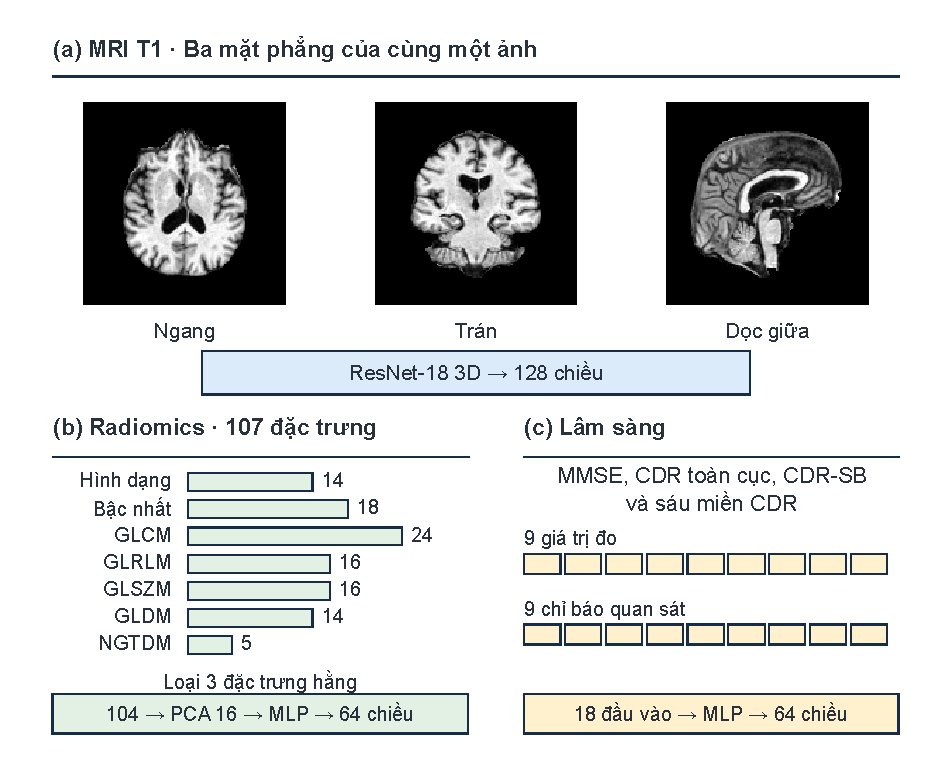
\includegraphics[width=\textwidth]{image/input-three-sources.pdf}
\caption{Minh họa ba nguồn dữ liệu đầu vào và các biểu diễn đặc trưng}
\label{fig:input-three-sources}
\end{figure}






\subsection{MRI và bộ mã hóa dùng chung}
Mỗi người tham gia có ba ảnh cộng hưởng từ có trọng số T1 (MRI T1-weighted), ghi nhận cấu trúc não ở ba lần khám. Ngay cả khi hình dạng một cấu trúc chưa thay đổi, vị trí của nó trên ảnh vẫn có thể khác giữa hai lần chụp. Chẳng hạn, nếu người tham gia hơi nghiêng đầu ở lần chụp thứ hai, hồi hải mã trái có thể xuất hiện ở vị trí khác so với lần đầu. Khi đối chiếu hai ảnh, độ lệch do tư thế đầu dễ bị nhầm với thay đổi hình thái mà mô hình cần khai thác, chẳng hạn như teo hồi hải mã hoặc giãn não thất. Vì vậy, tôi đưa ba ảnh về cùng hệ tọa độ và lưới lấy mẫu, đồng thời chuẩn hóa thang cường độ riêng cho từng ảnh. Hình~\ref{fig:mri-preprocessing} tóm tắt quy trình từ ba lần chụp đến đầu vào của nhánh ảnh.

\begin{figure}[H]
\centering
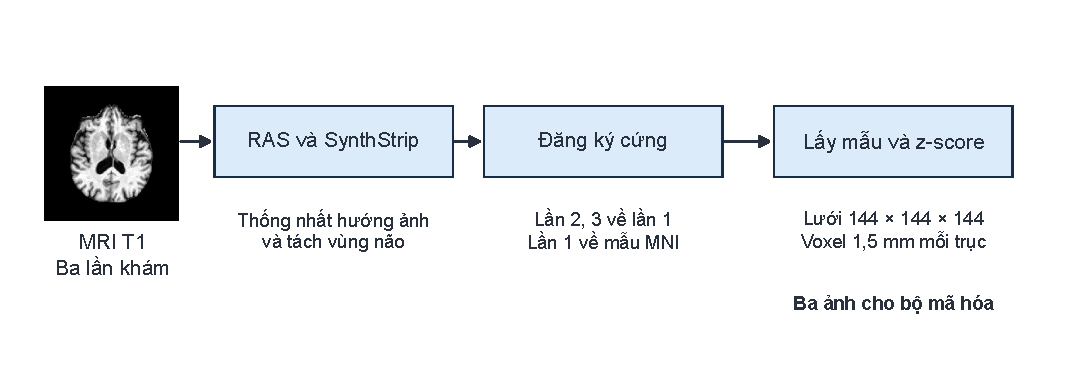
\includegraphics[width=\textwidth]{image/mri-preprocessing.pdf}
\caption{Quy trình tiền xử lý chuỗi ảnh MRI T1 dọc}
\label{fig:mri-preprocessing}
\end{figure}

\noindent\textbf{Chuẩn hóa hướng ảnh và tách não.}
Mỗi ảnh MRI là một khối dữ liệu ba chiều. Mỗi phần tử, gọi là voxel, mang một giá trị cường độ tại một vị trí trên lưới. Do các ảnh có thể được lưu theo những quy ước hướng khác nhau, trước tiên tôi đưa chúng về quy ước RAS (\emph{Right--Anterior--Superior}). Theo quy ước này, ba chiều dương lần lượt hướng về bên phải, phía trước và phía trên của người được chụp. Sau bước này, các trục có cùng ý nghĩa giải phẫu, nhưng tư thế đầu giữa các lần chụp vẫn có thể khác nhau.

Trên ảnh có cả não, hộp sọ, da đầu và các mô xung quanh. Tôi dùng SynthStrip, một phương pháp học sâu, để xác định vùng não cần giữ lại \cite{hoopes2022synthstrip}. Kết quả là một mặt nạ não (\emph{brain mask}) có cùng vị trí không gian với ảnh: voxel mang giá trị 1 thuộc vùng cần giữ, còn voxel mang giá trị 0 nằm ngoài vùng đó. Mặt nạ xác định phạm vi lấy số liệu cho bước chuẩn hóa cường độ. Đây là mặt nạ chung của vùng não, không phân biệt riêng chất xám, chất trắng hay dịch não tủy.

\noindent\textbf{Căn chỉnh giữa các lần khám.}
Tôi chọn ảnh MRI đầu tiên của mỗi người làm ảnh tham chiếu, rồi căn chỉnh riêng ảnh thứ hai và ảnh thứ ba về ảnh đầu bằng phép đăng ký cứng (\emph{rigid registration}). Phép biến đổi này có sáu bậc tự do: ba phép tịnh tiến dọc theo các trục không gian và ba phép quay quanh các trục đó. Nếu ở lần chụp thứ hai đầu vừa dịch sang bên vừa nghiêng, thành phần tịnh tiến điều chỉnh độ lệch vị trí, còn thành phần quay điều chỉnh góc nghiêng. Với một điểm có tọa độ $\mathbf{x}$ trong ảnh cần căn chỉnh, tọa độ tương ứng $\mathbf{x}'$ trong hệ tham chiếu được biểu diễn bởi
\[
 \mathbf{x}'=\mathbf{R}\mathbf{x}+\mathbf{t},
\]
trong đó $\mathbf{R}$ là ma trận quay và $\mathbf{t}$ là vectơ tịnh tiến. Cùng một phép quay và tịnh tiến tác động lên toàn bộ ảnh nên khoảng cách giữa hai điểm bất kỳ trong ảnh được bảo toàn. Nhờ đó, có thể đối chiếu vị trí hồi hải mã hay não thất giữa các lần chụp mà phép căn chỉnh không co giãn từng cấu trúc để ép chúng trùng khớp.

\noindent\textbf{Đưa chuỗi ảnh về hệ tọa độ MNI.}
Sau khi hai ảnh chụp sau đã có mốc tham chiếu là ảnh đầu, mỗi người vẫn có một mốc riêng. Để các chuỗi ảnh của nhiều người có chung hệ tọa độ, tôi căn chỉnh ảnh đầu của từng người về mẫu não tham chiếu MNI152NLin2009cAsym, cũng bằng phép đăng ký cứng sáu bậc tự do. Hình~\ref{fig:mri-registration} minh họa quan hệ giữa hai bước. Đối với một điểm trên ảnh lần hai, vị trí của nó được quy chiếu về ảnh lần đầu, rồi từ hệ tọa độ của ảnh lần đầu sang hệ tọa độ MNI. Quan hệ này cũng áp dụng cho ảnh lần ba. Như vậy, ảnh đầu làm mốc so sánh giữa các lần khám của một người, còn mẫu MNI làm mốc chung giữa những người tham gia.

\begin{figure}[H]
\centering
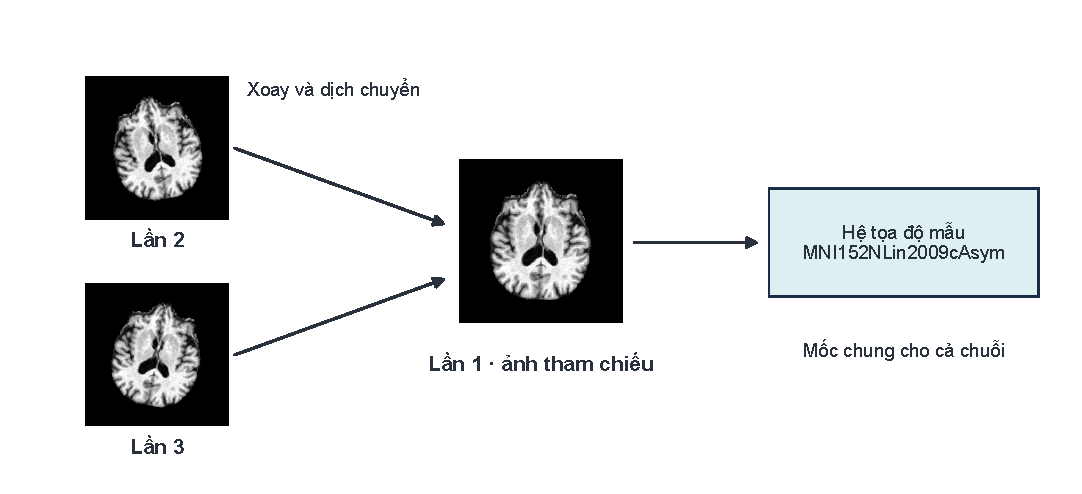
\includegraphics[width=\textwidth]{image/mri-registration.pdf}
\caption{Quy trình căn chỉnh không gian MRI giữa các lần khám và về mẫu MNI}
\label{fig:mri-registration}
\end{figure}

Phép đăng ký cứng giữ nguyên hình dạng và kích thước hình học của não. Quy trình không dùng biến đổi affine có thành phần co giãn hoặc biến dạng xiên, cũng không dùng đăng ký phi tuyến để làm biến dạng cục bộ. Lựa chọn này giới hạn những thay đổi hình học do bước căn chỉnh đưa vào ảnh. Vì hình dạng não tự nhiên khác nhau giữa các cá thể, việc dùng chung hệ tọa độ MNI không bảo đảm ranh giới của mọi cấu trúc giải phẫu đều trùng nhau giữa hai người.

\noindent\textbf{Lấy mẫu lại ảnh và mặt nạ.}
Sau căn chỉnh, ba ảnh của mỗi người được biểu diễn trên một lưới chung $144\times144\times144$ voxel. Kích thước voxel là 1.5~mm theo cả ba trục, tức là khoảng cách giữa tâm hai voxel kề nhau dọc một trục bằng 1.5~mm. Khi lấy mẫu lại (\emph{resampling}), tâm voxel trên lưới mới có thể nằm giữa các vị trí đã lấy mẫu trên ảnh ban đầu. Đối với ảnh MRI, tôi dùng nội suy tuyến tính để ước lượng cường độ từ các voxel lân cận. Chẳng hạn, trong ví dụ một chiều, nếu hai vị trí liền kề có cường độ 100 và 200 thì giá trị nội suy ở chính giữa là 150.

Với mặt nạ nhị phân, nội suy như vậy có thể tạo ra giá trị nằm giữa 0 và 1, làm mất ý nghĩa của nhãn vùng não. Thay vào đó, tôi dùng nội suy láng giềng gần nhất (\emph{nearest-neighbor interpolation}): mỗi voxel trên lưới mới nhận nhãn của voxel nguồn gần nhất. Nhờ vậy, ảnh và mặt nạ cùng nằm trên lưới đầu ra, còn mặt nạ vẫn chỉ nhận giá trị 0 hoặc 1.

\noindent\textbf{Chuẩn hóa cường độ trong vùng não.}
Cường độ MRI T1 mang tính tương đối: cùng một loại mô có thể cho giá trị khác nhau giữa hai lần chụp do thiết bị hoặc thiết lập thu nhận. Để giảm khác biệt về thang cường độ, tôi chuẩn hóa z-score riêng cho từng ảnh. Gọi $I(v)$ là cường độ tại voxel $v$ bên trong mặt nạ, còn $\mu$ và $\sigma$ lần lượt là trung bình và độ lệch chuẩn tính trên tất cả các voxel thuộc mặt nạ của chính ảnh đó. Với $\sigma>0$, cường độ sau chuẩn hóa là
\[
 z(v)=\frac{I(v)-\mu}{\sigma}.
\]
Chẳng hạn, nếu $\mu=100$, $\sigma=20$ và $I(v)=130$ thì $z(v)=(130-100)/20=1.5$. Giá trị này cho biết cường độ tại voxel đang xét cao hơn trung bình trong vùng não của ảnh 1.5 độ lệch chuẩn. Sau chuẩn hóa, cường độ trong mặt nạ có trung bình bằng 0 và độ lệch chuẩn bằng 1. Các voxel ngoài mặt nạ không tham gia tính hai thống kê này và được đặt bằng 0 ở ảnh đầu ra.

Tóm lại, bước chuẩn hóa z-score chỉ đồng nhất thang đo độ sáng tối giữa các ảnh chụp khác nhau mà hoàn toàn không làm thay đổi vị trí hay hình học của các voxel trong não. Trong quy trình này, tôi không áp dụng thêm bước khử nhiễu từ trường N4 (\emph{N4 bias field correction} — một kỹ thuật thường dùng để làm phẳng độ chênh lệch ánh sáng cục bộ do cuộn cảm máy chụp), nhằm tránh làm biến dạng độ tương phản mô tự nhiên của ảnh gốc. 

Như vậy, sau toàn bộ chuỗi tiền xử lý từ tách não, căn chỉnh tọa độ cho đến chuẩn hóa cường độ, bộ mã hóa sẽ tiếp nhận ba khối ảnh MRI đã được đưa về cùng một chuẩn thống nhất: cùng kích thước lưới $144\times144\times144$, cùng hệ tọa độ giải phẫu MNI, và cùng một thang đo giá trị. Nhờ loại bỏ được các yếu tố gây nhiễu ngoại cảnh như tư thế nghiêng đầu của người bệnh hay sự khác biệt về cài đặt máy chụp giữa các lần tái khám, mô hình học sâu có thể tập trung tối đa vào việc trích xuất những biến đổi giải phẫu bệnh lý thực sự — đặc biệt là hiện tượng teo mô não và giãn rộng não thất — diễn ra qua ba lần khám.

Sau tiền xử lý, cả ba MRI dùng chung bộ mã hóa ResNet-18 3D triển khai bằng MONAI, khởi tạo từ trọng số MedicalNet; sau đây gọi ngắn là ResNet-18 3D \cite{he2016deep,cardoso2022monai}. Mỗi tầng trong bốn tầng của mạng có hai khối cơ bản (BasicBlock), mỗi khối gồm hai phép tích chập với nhân $3^3$, chuẩn hóa BatchNorm, hàm kích hoạt ReLU và đường nối phần dư \cite{ioffe2015batchnorm,nair2010rectified}. Số kênh của bốn tầng lần lượt là 64, 128, 256 và 512. Sau gộp toàn cục, vectơ 512 chiều qua lớp tuyến tính $512\to128$, GELU, Dropout 0.20 và LayerNorm để tạo $M$ \cite{hendrycks2016gelu,srivastava2014dropout,ba2016layernorm}. Khi khởi tạo bộ mã hóa bằng trọng số MedicalNet từ Med3D \cite{chen2019med3d}, tôi nạp đầy đủ trọng số và trạng thái BatchNorm của mạng trích xuất đặc trưng, đồng thời bỏ khối đầu ra tiền huấn luyện. Toàn mạng được tinh chỉnh ngay từ vòng huấn luyện đầu tiên.

Bảng~\ref{tab:mri-encoder-shapes} trình bày kích thước bản đồ đặc trưng theo cấu hình MONAI (phiên bản 1.5.2)\footnote{Mã nguồn phiên bản: \url{https://github.com/Project-MONAI/MONAI/blob/1.5.2/monai/networks/nets/resnet.py}.}. Mỗi bản đồ đặc trưng có dạng $[B,C_{\mathrm{ch}},D,H,W]$, trong đó $B$ là cỡ lô, $C_{\mathrm{ch}}$ là số kênh và $D,H,W$ là ba kích thước không gian. Ký hiệu $C$ dùng riêng cho nhánh lâm sàng. Cả ba lần khám dùng chung bộ mã hóa. Sau bước gộp, các vectơ được xếp thành chuỗi $[B,T,F]$ trước phép chiếu, với $T=3$ là số lần khám và $F$ là số chiều đặc trưng.

\begin{table}[H]
\centering
\small
\caption{Kích thước đặc trưng trong bộ mã hóa MRI}
\label{tab:mri-encoder-shapes}
\begin{tabularx}{\textwidth}{@{}Y l@{}}
\toprule
\textbf{Bước} & \textbf{Kích thước đầu ra} \\
\midrule
MRI đầu vào & $[B,1,144,144,144]$ \\
Tích chập $7^3$, bước 1, đệm 3; BN; ReLU & $[B,64,144,144,144]$ \\
Gộp cực đại $3^3$, bước 2, đệm 1 & $[B,64,72,72,72]$ \\
Tầng ResNet 1: hai khối cơ bản & $[B,64,72,72,72]$ \\
Tầng 2: khối đầu có bước 2 & $[B,128,36,36,36]$ \\
Tầng 3: khối đầu có bước 2 & $[B,256,18,18,18]$ \\
Tầng 4: khối đầu có bước 2 & $[B,512,9,9,9]$ \\
Gộp trung bình toàn cục; trải phẳng & $[B,512,1,1,1]\to[B,512]$ \\
Xếp ba vectơ sau gộp & $[B,3,512]$ \\
Tuyến tính; GELU; Dropout; LayerNorm & $[B,3,128]$ \\
\bottomrule
\end{tabularx}
\end{table}

\subsection{Radiomics}
\label{sec:radiomics-pipeline}

Bên cạnh bộ mã hóa CNN học sâu — vốn trích xuất các biểu diễn ẩn trừu tượng từ ảnh khối 3D — tôi xây dựng một nhánh xử lý song song dựa trên \emph{Radiomics} để khai thác các đặc trưng hình học và kết cấu mô não được định nghĩa toán học tường minh \cite{vangriethuysen2017computational}. Trong khi mạng nơ-ron sâu thường hoạt động như một ``hộp đen'', các chỉ số radiomics mang ý nghĩa y sinh cụ thể, cho phép định lượng trực tiếp mức độ teo thoái hóa hình thái cũng như sự biến đổi vi mô về mật độ mô não của người bệnh.

\noindent\textbf{Trích xuất đặc trưng bằng PyRadiomics.}
Từ ảnh MRI đã qua tiền xử lý cùng mặt nạ não (\emph{brain mask}), tôi sử dụng thư viện chuẩn hóa PyRadiomics để trích xuất 107 đặc trưng định lượng thuộc bảy nhóm khác nhau (Bảng~\ref{tab:radiomics-groups}). Các nhóm này bao gồm:
\begin{itemize}
\item \emph{Đặc trưng hình dạng} (14 biến): Đo lường kích thước hình học tổng thể của vùng não, chẳng hạn như thể tích não thật (\emph{MeshVolume}) và diện tích bề mặt (\emph{SurfaceArea}).
\item \emph{Thống kê cường độ bậc nhất} (18 biến): Mô tả phân bố độ sáng tối của các voxel trong não mà không xét đến vị trí không gian, ví dụ như giá trị trung bình (\emph{Mean}), độ lệch chuẩn, độ bất đối xứng (\emph{Skewness}) và độ hỗn loạn (\emph{Entropy}).
\item \emph{Các nhóm kết cấu không gian} (75 biến): Nắm bắt mối tương quan không gian và độ thô mịn giữa các voxel lân cận thông qua các ma trận toán học kinh điển, bao gồm ma trận đồng xuất hiện mức xám (GLCM, 24 biến), ma trận độ dài dải mức xám (GLRLM, 16 biến), ma trận kích thước vùng mức xám (GLSZM, 16 biến), ma trận phụ thuộc mức xám (GLDM, 14 biến) và ma trận chênh lệch độ xám theo vùng lân cận (NGTDM, 5 biến).
\end{itemize}

\noindent\textbf{Chuẩn hóa cường độ riêng cho Radiomics.}
Một điểm kỹ thuật then chốt cần phân biệt rõ là sự khác biệt về yêu cầu đầu vào giữa nhánh CNN và nhánh Radiomics:
\begin{itemize}
\item \emph{Nhánh CNN (ResNet-18 3D)} tiếp nhận ảnh đã qua chuẩn hóa z-score (trung bình 0, độ lệch chuẩn 1), vì đây là dạng phân phối tối ưu giúp gradient lan truyền ổn định trong các mạng nơ-ron sâu.
\item \emph{Nhánh Radiomics} lại đòi hỏi một cách tiếp cận khác: các thuật toán tính ma trận kết cấu (như GLCM hay GLSZM) bắt buộc phải chia dải cường độ của ảnh thành một số lượng mức xám rời rạc cố định (\texttt{binCount=64}). Để các mức xám này có cùng khoảng chia và giữ đúng ý nghĩa vật lý giữa các bệnh nhân khác nhau, toàn bộ cường độ voxel trong mặt nạ trước hết được co giãn Min-Max tuyến tính về khoảng $[0, 1]$ (voxel tối nhất bằng 0, sáng nhất bằng 1). Nếu dùng ảnh z-score (vốn có cả giá trị âm lẫn dương và biên độ biến thiên không bị chặn), việc chia 64 mức xám sẽ bị xáo trộn giữa các lần chụp, dẫn đến các phép đo kết cấu bị sai lệch.
\end{itemize}

\noindent\textbf{Lọc biến hằng và giảm chiều bằng PCA.}
Do toàn bộ voxel trong não đã được chuẩn hóa về dải $[0, 1]$, ba đặc trưng thống kê bậc nhất — bao gồm giá trị cường độ nhỏ nhất (luôn bằng 0), giá trị lớn nhất (luôn bằng 1) và khoảng biến thiên cường độ (luôn bằng $1-0=1$) — trở thành các giá trị hằng số giống hệt nhau ở mọi người tham gia. Vì không chứa thông tin phân biệt bệnh lý, ba biến này được loại bỏ, giữ lại chính xác 104 đặc trưng thực sự hữu ích.

Trong số 104 đặc trưng còn lại, nhiều biến có mức độ tương quan chéo cao (chẳng hạn các đặc trưng đo kích thước não hoặc các chỉ số đồng nhất kết cấu). Để loại bỏ hiện tượng đa cộng tuyến và tránh bùng nổ tham số khi kết hợp với các nguồn dữ liệu khác, tôi áp dụng Phân tích thành phần chính (PCA) \cite{jolliffe2016pca}. Nhằm triệt tiêu hoàn toàn nguy cơ rò rỉ dữ liệu, các tham số chuẩn hóa z-score của từng đặc trưng và ma trận chuyển đổi PCA đều được ước lượng nghiêm ngặt trên tập huấn luyện, sau đó mới áp dụng cố định cho tập xác thực và kiểm tra. Với ngưỡng giữ lại ít nhất 99\% tổng phương sai, mô hình xác định được đúng 16 thành phần chính tại mỗi lần khám.

\noindent\textbf{Tạo biểu diễn nhúng qua mạng MLP.}
Cuối cùng, vectơ 16 chiều sau PCA được đưa qua một khối mạng perceptron đa tầng ($16 \to 128 \to 64$) gồm kích hoạt phi tuyến GELU, tỉ lệ Dropout 0.20 và lớp chuẩn hóa LayerNorm \cite{hendrycks2016gelu,srivastava2014dropout,ba2016layernorm}. Đầu ra của khối này là một vectơ biểu diễn Radiomics $R \in \mathbb R^{64}$, vừa cô đọng các dấu hiệu giải phẫu vi mô, vừa đồng bộ kích thước để sẵn sàng tham gia vào các tầng hợp nhất đa phương thức tiếp theo.

\begin{table}[H]
\centering\small
\caption[Các nhóm đặc trưng radiomics]{Bảy nhóm đặc trưng radiomics trích từ ảnh và mặt nạ toàn não. Cột cuối nêu ví dụ thuộc từng nhóm.}
\label{tab:radiomics-groups}
\begin{tabularx}{\linewidth}{@{}L{2.7cm}r Y Y@{}}
\toprule
Nhóm & Số lượng & Thông tin mô tả & Ví dụ \\
\midrule
Hình dạng & 14 & Hình học của mặt nạ não & Thể tích (MeshVolume), diện tích bề mặt (SurfaceArea) \\
Thống kê bậc nhất & 18 & Phân bố cường độ trong mặt nạ & Trung bình (Mean), phương sai (Variance), Entropy \\
GLCM & 24 & Quan hệ mức xám giữa các cặp voxel & Contrast, Correlation \\
GLRLM & 16 & Độ dài chuỗi voxel cùng mức xám theo hướng & ShortRunEmphasis, LongRunEmphasis \\
GLSZM & 16 & Kích thước vùng liên thông cùng mức xám & SmallAreaEmphasis, LargeAreaEmphasis \\
GLDM & 14 & Mức phụ thuộc cường độ giữa voxel và lân cận & DependenceEntropy, DependenceVariance \\
NGTDM & 5 & Chênh lệch cường độ với lân cận & Coarseness, Contrast, Busyness, Complexity, Strength \\
\midrule
Tổng & 107 & Còn 104 sau khi loại Maximum, Minimum và Range & PCA giữ 16 thành phần \\
\bottomrule
\end{tabularx}
\end{table}


\subsection{Dữ liệu lâm sàng và chỉ báo có dữ liệu}
Trong chín biến dự báo của nhánh lâm sàng, ba biến tổng hợp gồm MMSE-total, CDR-global và tổng điểm các miền CDR (CDR-sum-of-boxes, CDR-SB). Sáu biến còn lại là điểm của từng miền CDR, bao gồm trí nhớ, định hướng, phán đoán, hoạt động cộng đồng, sinh hoạt gia đình và sở thích, cùng khả năng tự chăm sóc \cite{folstein1975mmse,morris1993cdr}. Tôi điền mỗi giá trị thiếu bằng trung vị của biến tại lần khám tương ứng trên tập huấn luyện. Nếu toàn bộ số đo của biến đều thiếu ở lần khám đó, tôi dùng trung vị của biến trên toàn tập huấn luyện. Sau khi điền thiếu, tôi chuẩn hóa các giá trị theo trung bình và độ lệch chuẩn ước lượng từ tập huấn luyện. Để mô hình phân biệt số đo thực tế với giá trị được điền thay, mỗi biến có một chỉ báo nhị phân bằng 1 nếu có số đo và bằng 0 nếu thiếu trước khi điền. Nhờ kết hợp chín giá trị lâm sàng với chín chỉ báo tương ứng, nhánh lâm sàng có đầu vào 18 chiều để đưa qua MLP $18\to64\to64$ với GELU, Dropout 0.10 và LayerNorm, tạo biểu diễn lâm sàng $C\in\mathbb R^{64}$.

Bảng~\ref{tab:clinical-inputs} liệt kê từng biến để phân biệt chín giá trị lâm sàng với chín chỉ báo dữ liệu thiếu. CDR-global và CDR-SB là hai cách tổng hợp khác nhau; sáu miền CDR vẫn được giữ riêng để mô hình nhận thông tin cụ thể của từng hoạt động.
\begin{table}[H]
\centering\small
\caption[Chín biến lâm sàng đầu vào]{Chín giá trị trước khi chuẩn hóa, theo đúng thứ tự đầu vào của mô hình. Mỗi giá trị có thêm một chỉ báo quan sát tương ứng.}
\label{tab:clinical-inputs}
\begin{tabularx}{\linewidth}{@{}r L{3.6cm}Y@{}}
\toprule
Vị trí & Biến lâm sàng & Ý nghĩa \\
\midrule
1 & MMSE-total & Tổng điểm đánh giá nhận thức, thang 0--30 \\
2 & CDR-global & Mức độ suy giảm nhận thức và chức năng tổng thể \\
3 & CDR-SB & Tổng điểm của sáu miền CDR, thang 0--18 \\
4 & CDR: trí nhớ & Khả năng ghi nhớ và nhớ lại thông tin \\
5 & CDR: định hướng & Nhận biết thời gian, địa điểm và hoàn cảnh \\
6 & CDR: phán đoán & Khả năng phán đoán và giải quyết vấn đề \\
7 & CDR: cộng đồng & Khả năng tham gia hoạt động ngoài gia đình \\
8 & CDR: gia đình/sở thích & Khả năng thực hiện công việc tại nhà và duy trì sở thích \\
9 & CDR: tự chăm sóc & Mức độc lập trong chăm sóc bản thân \\
\bottomrule
\end{tabularx}
\end{table}


Hình~\ref{fig:clinical-18} minh họa cách hình thành đầu vào 18 chiều. Khi một biến thiếu số đo, nhánh giá trị nhận giá trị đã điền và chuẩn hóa nhưng chỉ báo vẫn bằng 0, trong khi chỉ báo của biến có số đo bằng 1. Nhờ vậy, mô hình vẫn phân biệt được hai trường hợp ngay cả khi chúng có cùng giá trị số sau xử lý.

\begin{figure}[H]
\centering
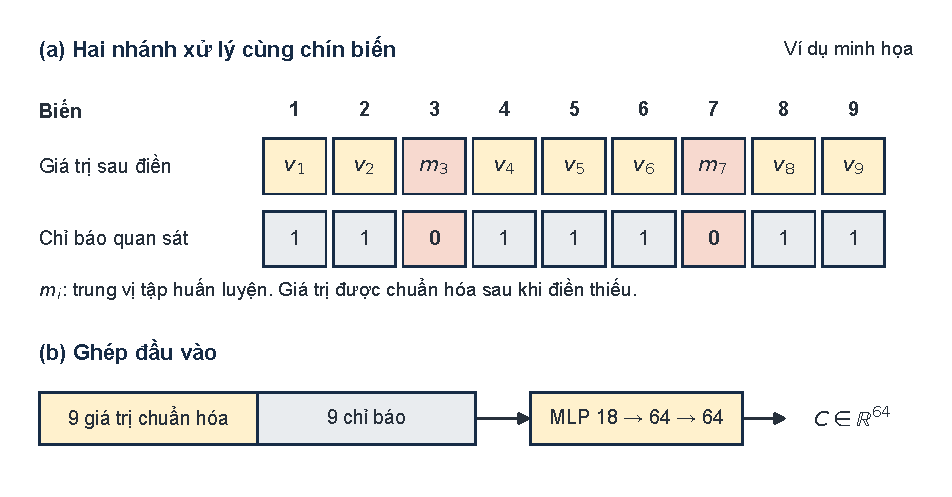
\includegraphics[width=\textwidth]{image/clinical-18-inputs.pdf}
\caption{Quy trình mở rộng chín biến lâm sàng thành 18 chiều đầu vào}
\label{fig:clinical-18}
\end{figure}

\section{Các mô hình tham chiếu}
\label{sec:architecture-evolution}
Các mô hình tham chiếu giúp trả lời hai câu hỏi: thông tin theo thời gian đóng góp thế nào, và cách kết hợp các nguồn ảnh hưởng ra sao đến dự đoán. Nhóm MRI gồm mô hình dùng ảnh cuối, mô hình dùng chuỗi MRI với trạng thái cuối của T-LSTM, và mô hình dùng T-LSTM kết hợp attention để tổng hợp cả ba trạng thái. Nhóm hợp nhất dùng cùng ba nguồn MRI, radiomics và lâm sàng, lần lượt kết hợp bằng ghép nối, tích ngoài và CP.

Một đối chứng riêng được xây dựng theo quy trình CNN--PCA--T-LSTM của Aghajanian và cộng sự \cite{aghajanian2025longitudinal}. CNN TensorFlow nhận MRI kích thước $128^3$ và xuất vectơ 512 chiều trước Dropout và lớp đầu ra. PCA được học từ tập huấn luyện với ngưỡng giữ ít nhất 99\% phương sai, không chuẩn hóa thang đo hoặc làm trắng. Chuỗi đặc trưng sau PCA được đưa vào T-LSTM có trạng thái ẩn 64 chiều.

Với các mã khởi tạo 20260727, 20260728 và 20260729, số thành phần PCA tương ứng là 38, 69 và 2. Ở lần chạy thứ ba, hai thành phần đầu đã giữ 99.47\% phương sai của 753 biểu diễn huấn luyện, nên đáp ứng ngưỡng 99\%. Phương sai tập trung rất mạnh vào hai hướng ở lần khởi tạo thứ ba, cho thấy số chiều hiệu dụng của biểu diễn CNN nhạy với khởi tạo. Mục~\ref{sec:paper-adaptation-results} đối chiếu số chiều này với C-index của từng lần khởi tạo. Bảng~\ref{tab:reference-methods} tóm tắt dữ liệu và vai trò của phương pháp gốc, bản tái lập có điều chỉnh và mô hình chính.

\begin{table}[H]
\centering\small
\caption[Phân biệt công trình gốc, bản tái lập có điều chỉnh và phương pháp chính]{Dữ liệu, cấu hình và vai trò của ba phương pháp.}
\label{tab:reference-methods}
\begin{tabularx}{\textwidth}{@{}L{3.2cm}Y Y@{}}
\toprule
\textbf{Phương pháp} & \textbf{Dữ liệu và tiền xử lý} & \textbf{Mô hình và vai trò} \\
\midrule
Aghajanian gốc \cite{aghajanian2025longitudinal} & 228 người có MCI; SPM12, mô não và radiomics chất xám & CNN--PCA--T-LSTM; huấn luyện hai bước; nguồn tham chiếu \\
Bản tái lập có điều chỉnh & 359 người; ảnh MRI đã cố định được đổi kích thước cho CNN & CNN/PCA theo lần khởi tạo; T-LSTM 64; mô hình đối chứng \\
RC-Free Pairwise & 359 người; MRI $144^3$, radiomics toàn não, lâm sàng và chỉ báo có dữ liệu & MedicalNet; CP MR/MC; phần dư có cổng; T-LSTM 128; kiến trúc chính \\
\bottomrule
\end{tabularx}
\end{table}

Về triển khai, mô hình chính dùng PyTorch và MONAI; scikit-learn thực hiện các biến đổi dữ liệu bảng \cite{paszke2019pytorch,cardoso2022monai,pedregosa2011sklearn}. Bản CNN--PCA--T-LSTM có bộ tối ưu, cỡ lô và cách tính hàm mất mát Cox khác nhóm mô hình tương tác theo cặp. C-index được tính thống nhất để đối chiếu hiệu năng tổng thể của các quy trình.

\section{Mô hình đối chứng ghép nối đặc trưng}
Đối chứng ghép nối được xây dựng để khảo sát đóng góp của tương tác theo cặp trong điều kiện giữ nguyên cả ba nguồn dữ liệu đầu vào. Tại mỗi lần khám, tôi ghép vectơ MRI $M_t$ có 128 chiều, vectơ radiomics $R_t$ có 64 chiều và vectơ lâm sàng $C_t$ có 64 chiều theo đúng thứ tự này. Khối MLP nhận vectơ chung 256 chiều và ánh xạ thành biểu diễn 128 chiều cho khối thời gian. Phép ghép nối tại lần khám $t$ có dạng
\begin{equation}
 F_t=\operatorname{MLP}_{\rm out}(M_t\concat R_t\concat C_t),\qquad
 M_t\concat R_t\concat C_t\in\mathbb R^{256},\quad F_t\in\mathbb R^{128}.\label{eq:concat}
\end{equation}
Khối đầu ra $\operatorname{MLP}_{\rm out}$ gồm lớp tuyến tính $256\to128$, GELU, Dropout 0.20 và LayerNorm. Chuỗi ba $F_t$ đi qua khối thời gian và khối dự báo Cox. Các lớp sau ghép nối học quan hệ giữa các nguồn từ vectơ chung này.


\begin{figure}[H]
\centering
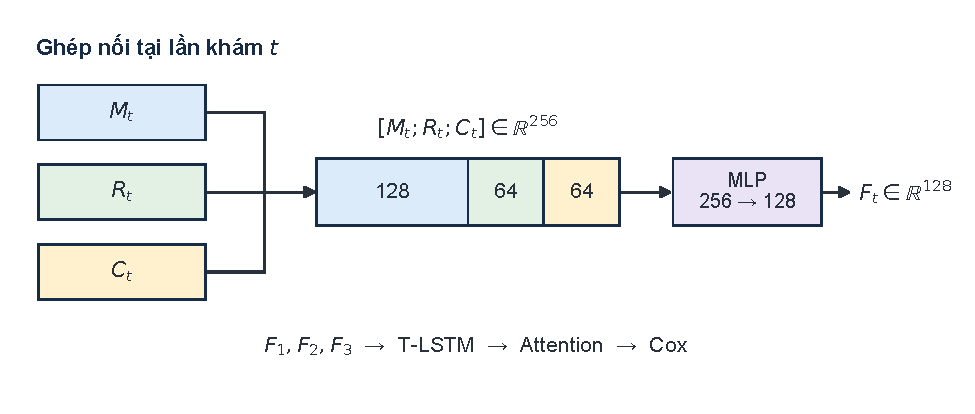
\includegraphics[width=\textwidth]{image/concat-baseline.pdf}
\caption[Mô hình đối chứng ghép nối]{Luồng tính của mô hình đối chứng ghép nối.}
\label{fig:concat-baseline}
\end{figure}
Mô hình theo cặp bổ sung một khối riêng để biểu diễn các tích chéo trước bước ghép nối. Khi so sánh hai cách hợp nhất, tôi giữ nguyên các phần chung và dùng cùng trọng số ban đầu cho các phần này. Mục~\ref{sec:matched-fusion} trình bày kết quả đối chiếu này.

\Needspace{9\baselineskip}
\section{Hợp nhất động qua tương tác theo cặp}
\label{sec:pair-fusion}
Từ cùng ba biểu diễn đầu vào như đối chứng ghép nối, mô hình đầy đủ kết hợp từng cặp tại mỗi lần khám để tạo ba tương tác MR, MC và RC. Trước khi tính tương tác, ba phép chiếu tuyến tính không có hệ số chệch giảm $M$ từ 128 xuống 32 chiều, $R$ từ 64 xuống 32 chiều và $C$ từ 64 xuống 16 chiều:
\begin{equation}
 \widetilde M\in\mathbb R^{32},\qquad
 \widetilde R\in\mathbb R^{32},\qquad
 \widetilde C\in\mathbb R^{16}.\label{eq:input-projection}
\end{equation}

\begin{figure}[H]
\centering
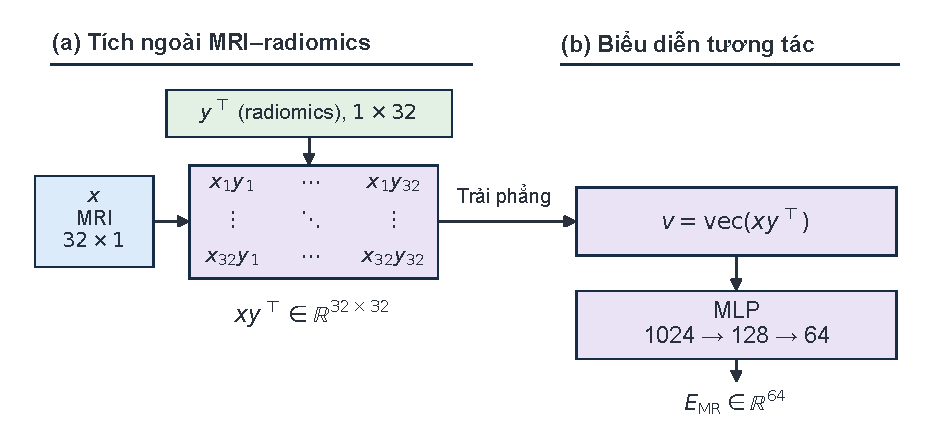
\includegraphics[width=\textwidth]{image/mr-outer-product.pdf}
\caption{Phép tích ngoài đầy đủ và khối MLP tương tác}
\label{fig:mr-outer-product}
\end{figure}

Với mỗi cặp tương tác $k\in\{\mathrm{MR},\mathrm{MC},\mathrm{RC}\}$, tôi ký hiệu hai vectơ đầu vào là $x\in\mathbb R^{d_x\times1}$ và $y\in\mathbb R^{d_y\times1}$, tương ứng với hai biểu diễn đã giảm chiều lấy từ $(\widetilde M,\widetilde R,\widetilde C)$. Tích ngoài $xy^\top\in\mathbb R^{d_x\times d_y}$ tạo ra ma trận chứa tích của từng tọa độ của $x$ với từng tọa độ của $y$, sau đó mô hình trải phẳng ma trận thành vectơ $v=\operatorname{vec}(xy^\top)$ để đưa vào MLP. Do số chiều đầu vào khác nhau giữa các cặp, MR tạo ra $32\times32=1024$ giá trị tương tác, trong khi MC và RC mỗi cặp tạo ra $32\times16=512$ giá trị.

MLP của mỗi cặp ánh xạ vectơ vừa trải phẳng thành biểu diễn tương tác: MR dùng $1024\to128\to64$, MC dùng $512\to128\to64$, RC dùng $512\to64\to32$. Giữa hai lớp tuyến tính có GELU và Dropout 0.10; LayerNorm đặt cuối mỗi khối.

Xét cặp MRI và radiomics (MR) của một người tại một lần khám. Sau khi xử lý cặp này, MLP cho một vectơ 64 chiều biểu diễn thông tin tương tác giữa hai nguồn. Mô hình dùng vectơ đó để bổ sung thông tin cho cả biểu diễn MRI $M$ và biểu diễn radiomics $R$. Vì phép cộng được thực hiện theo từng tọa độ, phần bổ sung phải có cùng số chiều với biểu diễn nhận nó.

Hình~\ref{fig:pair-update-routes} minh họa hai nhánh đi ra từ MR. Ở nhánh dẫn đến MRI, một lớp tuyến tính biến vectơ tương tác 64 chiều thành vectơ 128 chiều để có thể cộng vào $M$. Ở nhánh dẫn đến radiomics, một lớp tuyến tính khác ánh xạ từ 64 chiều sang 64 chiều. Dù số chiều đã khớp với $R$, lớp này vẫn học cách kết hợp các tọa độ của vectơ tương tác cho riêng nguồn radiomics. Sau phép chiếu, mỗi nhánh chuẩn hóa vectơ bằng LayerNorm riêng. Cổng của nhánh điều tiết mức đóng góp tại lần khám đang xét. Mô hình nhân vectơ đã chuẩn hóa với giá trị cổng và hệ số của nhánh trước khi cộng vào biểu diễn gốc.

\begin{figure}[H]
\centering
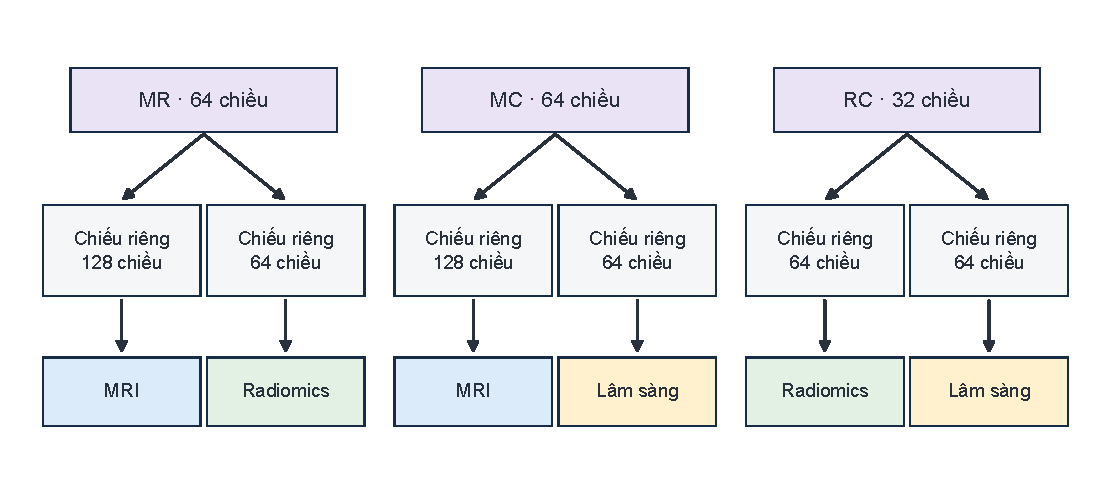
\includegraphics[width=\linewidth]{image/pair-update-routes.pdf}
\caption{Sơ đồ sáu nhánh cập nhật biểu diễn từ ba cặp tương tác}
\label{fig:pair-update-routes}
\end{figure}

Đọc sơ đồ theo nguồn nhận cho thấy MRI nhận thông tin từ MR và MC, radiomics nhận từ MR và RC, còn dữ liệu lâm sàng nhận từ MC và RC. Mỗi nguồn giữ vectơ gốc và cộng các phần bổ sung dành cho mình. Cả sáu nhánh đều sử dụng dữ liệu của cùng một người ở cùng một lần khám. Khi bỏ cặp RC, hai nhánh từ RC đến radiomics và lâm sàng cũng được bỏ. Trong RC-Free, radiomics vẫn nhận thông tin từ MR và dữ liệu lâm sàng vẫn nhận thông tin từ MC, nên cả ba nguồn tiếp tục tham gia vào biểu diễn hợp nhất.

\section{Tham số hóa tương tác theo cặp bằng CP}
\label{sec:cp-method}

Mặc dù phép hợp nhất tương tác song tuyến đầy đủ (Full Outer-Product) ở Mục~\ref{sec:pair-fusion} có khả năng bắt cặp tường minh các đặc trưng giữa hai phương thức, rào cản lớn nhất của nó nằm ở chi phí tính toán và số lượng tham số khổng lồ. Một lớp song tuyến đầy đủ đòi hỏi phải học một tensor trọng số ba chiều $\mathcal W\in\mathbb R^{d_h\times d_x\times d_y}$. Khi số chiều đặc trưng hoặc số kênh ẩn tăng lên, số lượng tham số này bùng nổ rất nhanh, không chỉ gây áp lực lớn lên bộ nhớ tính toán mà còn làm tăng nghiêm trọng nguy cơ quá khớp (overfitting) trên các bộ dữ liệu y tế vốn có cỡ mẫu hạn chế như ADNI.

Để giải quyết mâu thuẫn giữa năng lực biểu diễn tương tác và độ phức tạp tham số, tôi áp dụng kỹ thuật phân rã tensor CANDECOMP/PARAFAC (CP) \cite{kolda2009tensor,liu2018lowrank}. Nguyên lý cốt lõi của phân rã CP là xấp xỉ tensor trọng số ba chiều phức tạp thành tổng của $Q$ tích ngoài giữa các vectơ một chiều, trong đó $Q \ll \min(d_x d_y, d_h)$ là hạng phân rã (rank). Nhờ cấu trúc hạng thấp này, thay vì phải thực hiện tích ngoài tường minh trong không gian gốc, hai vectơ đặc trưng đầu vào trước hết được chiếu tuyến tính về một không gian tiềm ẩn thấp chiều ($Q$ chiều), sau đó nhân từng phần tử (Hadamard product) để tạo tương tác, rồi mới chiếu tiếp sang không gian ẩn $d_h$. Hình~\ref{fig:cp-block} minh họa trực quan luồng tính toán này cho cặp MR với hạng $Q=8$.

\begin{figure}[H]
\centering
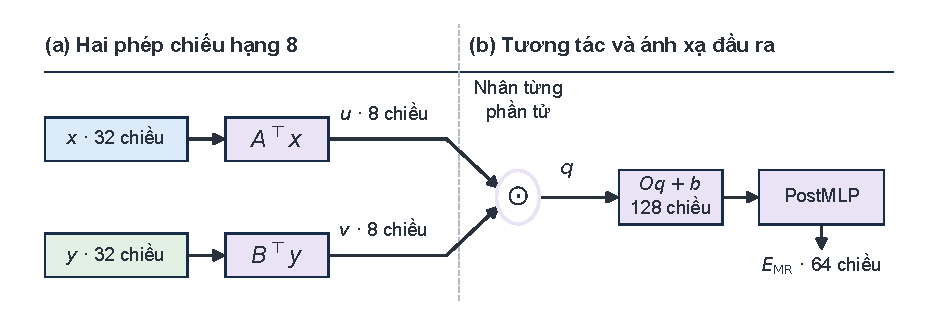
\includegraphics[width=\textwidth]{image/outer-vs-cp.pdf}
\caption{Luồng tính toán của khối tương tác CP hạng thấp}
\label{fig:cp-block}
\end{figure}
Với lớp đầy đủ, chiều ẩn thứ $s$ được tính bằng
\begin{equation}
 h_s=\sum_{i=1}^{d_x}\sum_{j=1}^{d_y}\mathcal W_{sij}x_i y_j+b_s,
 \qquad \mathcal W\in\mathbb R^{d_h\times d_x\times d_y}.
\end{equation}
Thay vì phải lưu trữ và học trực tiếp toàn bộ khối trọng số khổng lồ trên, CP tham số hóa \emph{tensor trọng số của ánh xạ song tuyến} thông qua các ma trận nhân tử hạng thấp \cite{kolda2009tensor,liu2018lowrank}:
\begin{equation}
 \mathcal W_{sij}\approx\sum_{q=1}^{Q}O_{sq}A_{iq}B_{jq}.
 \label{eq:cp-weight}
\end{equation}
Trong cách biểu diễn phân rã này, mạng chỉ cần học ba ma trận nhân tử $A\in\mathbb R^{d_x\times Q}$, $B\in\mathbb R^{d_y\times Q}$ và $O\in\mathbb R^{d_h\times Q}$. Quá trình tính toán thuận diễn ra hết sức tự nhiên và hiệu quả: hai vectơ đầu vào $x$ và $y$ được chiếu độc lập về không gian $Q$ chiều thông qua $A$ và $B$, tạo thành hai vectơ tọa độ $u$ và $v$; tiếp đó, phép nhân từng phần tử giữa $u$ và $v$ nắm bắt tương tác chéo giữa hai nguồn dữ liệu; cuối cùng, ma trận $O$ chiếu kết quả tương tác này lên không gian ẩn $d_h$:
\begin{align}
 u&=A^\top x,\qquad v=B^\top y,\qquad q=u\odot v,\label{eq:cp-lowrank}\\
 h&=Oq+b,\qquad E_k=\operatorname{PostMLP}_k(h),
 \label{eq:cpblock}
\end{align}
với $E_k$ là biểu diễn tương tác đầu ra của cặp $k\in\{\mathrm{MR},\mathrm{MC},\mathrm{RC}\}$. Cần lưu ý rằng các ma trận chiếu $A$ và $B$ không sử dụng hệ số chệch để bảo toàn tính đối xứng của phép nhân từng phần tử; hệ số chệch $b$ của lớp đầu được tích hợp trực tiếp vào phép chiếu đầu ra $Oq+b$. Khối mạng perceptron đa tầng phía sau ($\operatorname{PostMLP}_k$) vẫn giữ nguyên cấu trúc chuẩn hóa và phi tuyến gồm hàm kích hoạt GELU, Dropout 0.10, lớp tuyến tính $d_h\to d_o$ và chuẩn hóa LayerNorm. Nhờ vậy, mô hình đối chứng CP chỉ thay đổi duy nhất phép biến đổi tương tác đầu tiên, trong khi bảo lưu toàn bộ kích thước đầu ra, MLP phía sau, bộ mã hóa, các nhánh truyền phần dư, cổng điều tiết, hệ số điều chỉnh và khối thời gian. Cách bố trí này giúp cô lập hoàn toàn biến số nghiên cứu, bảo đảm rằng bất kỳ sự khác biệt nào về hiệu năng đều phản ánh chính xác hiệu quả của việc tham số hóa hạng thấp.



\begin{table}[H]
\centering
\caption{Cấu hình CP theo cặp tương tác}
\label{tab:cpconfig}
\begin{tabular}{lccccc}
\toprule
Cặp & $(d_x,d_y)$ & Hạng $Q$ & Chiều ẩn $d_h$ & Đầu ra $d_o$ & RC-Free \\
\midrule
MR & $(32,32)$ & 8 & 128 & 64 & Giữ \\
MC & $(32,16)$ & 8 & 128 & 64 & Giữ \\
RC & $(32,16)$ & 4 & 64 & 32 & Loại \\
\bottomrule
\end{tabular}
\end{table}

Bảng~\ref{tab:cpconfig} trình bày chi tiết cấu hình hạng CP và kích thước các lớp cho từng cặp tương tác. Việc ấn định hạng $Q=8$ cho hai cặp MR và MC cùng $Q=4$ cho cặp RC phản ánh sự cân đối có chủ đích giữa năng lực biểu diễn và kích thước đặc trưng của từng phương thức (cặp RC có số chiều đầu vào nhỏ hơn nên chỉ cần hạng thấp hơn).

Hiệu quả giảm độ phức tạp của phân rã CP có thể được định lượng rõ ràng qua sự khác biệt giữa hai công thức tham số: một lớp song tuyến đầy đủ đòi hỏi $d_h d_x d_y + d_h$ tham số (với độ phức tạp tăng theo tích $d_x d_y$), trong khi cách tham số hóa CP chỉ tiêu tốn $Q(d_x + d_y + d_h) + d_h$ tham số (với độ phức tạp chỉ tăng tuyến tính theo tổng $d_x + d_y$). Đây chính là nền tảng lý thuyết giải thích vì sao CP có thể \textbf{cắt giảm hơn 98\%} số lượng trọng số ở các lớp tương tác đầu tiên. Dẫu vậy, xét trên quy mô toàn mạng, bộ mã hóa hình ảnh 3D ResNet-18 vẫn chiếm phần lớn số tham số; do đó, vai trò cốt lõi của CP không chỉ là thu nhỏ mô hình tổng thể, mà quan trọng hơn là đóng vai trò như một cơ chế điều chuẩn (regularization) hiệu quả, ngăn chặn hiện tượng quá khớp ở chính các tầng hợp nhất đa phương thức.

\section{Truyền phần dư qua cổng điều tiết động}
\label{sec:gated-routing}

Sau khi đã trích xuất được đặc trưng tương tác từ các khối CP, bài toán kiến trúc cốt lõi tiếp theo là: \emph{Làm thế nào để truyền tải và tích hợp thông tin tương tác này vào biểu diễn của từng phương thức mà không làm suy hao hoặc sai lệch tín hiệu gốc?}

Trong mô hình đối chứng ghép nối thông thường, các đặc trưng được gộp cứng nhắc lại với nhau trước khi đưa vào mô hình thời gian. Cách tiếp cận này tiềm ẩn nhiều rủi ro trong bài toán y sinh: sự tương tác giữa các phương thức không phải lúc nào cũng mang lại giá trị gia tăng đồng đều ở mọi bệnh nhân hay mọi thời điểm thăm khám. Ở một số ca bệnh hoặc lần khám có độ nhiễu cao (chẳng hạn chất lượng ảnh MRI kém hoặc kết quả đo lâm sàng dao động), việc ép buộc mô hình tiếp nhận toàn bộ tín hiệu tương tác có thể làm xáo trộn các đặc trưng bệnh học vốn có của từng nguồn đơn lẻ.

Để khắc phục nhược điểm này, tôi đề xuất cơ chế \emph{kết nối phần dư qua cổng điều tiết động} (gated residual routing), kế thừa và phát triển từ các nguyên lý điều tiết phần dư trong học sâu đa phương thức \cite{ryumina2026residual,liu2026motion}. Triết lý của cơ chế này là bảo toàn nguyên vẹn ``đường truyền gốc'' (identity path) của từng phương thức, đồng thời xem thông tin tương tác như một lượng bổ chính phần dư có điều kiện. Nhờ đó, ngay cả khi tín hiệu tương tác bị nhiễu hoặc cổng điều tiết khép lại, mô hình vẫn duy trì được nguồn thông tin độc lập và tin cậy từ biểu diễn ban đầu.

Cơ chế điều tiết này được hiện thực hóa qua ba tầng xử lý chặt chẽ:
\begin{enumerate}
\item \emph{Phép chiếu tương thích theo phương thức đích}: Mỗi cặp tương tác $k$ (như MR hay MC) tạo ra một biểu diễn tương tác chung $E_k$. Tuy nhiên, do các phương thức đích $d$ có kích thước không gian đặc trưng khác nhau, đặc trưng $E_k$ trước tiên được chiếu về không gian của phương thức đích thông qua một ánh xạ tuyến tính và chuẩn hóa qua LayerNorm:
\begin{equation}
 \widehat E_{k\to d}=\LN_{k\to d}(W_{k\to d}E_k+b_{k\to d}).\label{eq:target-projection}
\end{equation}
Ánh xạ này sử dụng hệ số chệch để tăng tính linh hoạt khi dịch chuyển hệ tọa độ đặc trưng, trong khi bước giảm chiều trước CP hoàn toàn không dùng hệ số chệch. Cả hai bước đều không sử dụng hàm kích hoạt phi tuyến nhằm bảo toàn tuyến tính của tín hiệu trước khi vào cổng.

\item \emph{Cổng điều tiết động theo từng bệnh nhân}: Cổng $g_{k\to d}$ hoạt động như một chiếc ``van thông minh'', tiếp nhận đồng thời cả biểu diễn gốc đã chuẩn hóa của phương thức đích lẫn đặc trưng tương tác đã chiếu để đánh giá xem: với \emph{cá thể cụ thể này tại lần khám cụ thể này}, thông tin tương tác có thực sự hữu ích hay không:
\begin{equation}
 g_{k\to d}=\sigma\!\left(
 w_{k\to d}^{\top}\operatorname{GELU}\!\left[
 V_{k\to d}\bigl(\LN_d^{\rm gate}(U_d)\concat\widehat E_{k\to d}\bigr)
 +a_{k\to d}\right]+c_{k\to d}\right).
 \label{eq:dynamic-gate}
\end{equation}
Mạng MLP của mỗi cổng gồm một lớp ẩn 32 chiều với kích hoạt GELU và tạo ra một giá trị vô hướng trong khoảng $(0,1)$ thông qua hàm sigmoid độc lập. Việc sử dụng sigmoid riêng cho từng cổng (thay vì softmax trên tất cả các nhánh) mang ý nghĩa then chốt: các nhánh tương tác có thể cùng mở rộng nếu tất cả đều hữu ích, hoặc cùng khép lại nếu dữ liệu bị nhiễu, mà không bị ràng buộc phải chia sẻ một tổng trọng số cố định. Trọng số của cổng được khởi tạo theo phân phối Xavier~\cite{glorot2010understanding} với hệ số chệch ban đầu bằng không.

\item \emph{Hệ số tỉ lệ toàn cục học được}: Bên cạnh chiếc van động $g_{k\to d}$ điều chỉnh theo từng mẫu, mỗi nhánh còn được trang bị một hệ số vô hướng $\lambda_{k\to d}$ dùng chung cho toàn bộ tập dữ liệu và mọi mốc thời gian. Hệ số này được khởi tạo tại $\lambda=0.1$ và \emph{hoàn toàn không bị ràng buộc về dấu}. Nếu cổng $g$ quyết định độ mở tức thời theo ngữ cảnh của từng bệnh nhân, thì $\lambda$ đóng vai trò như một ``chiết áp nền'' học được trong quá trình tối ưu, xác định cường độ đóng góp tổng thể và chiều hướng tác động (tương hỗ tích cực hay triệt tiêu lẫn nhau) của toàn bộ nhánh truyền.
\end{enumerate}

\begin{figure}[H]
\centering
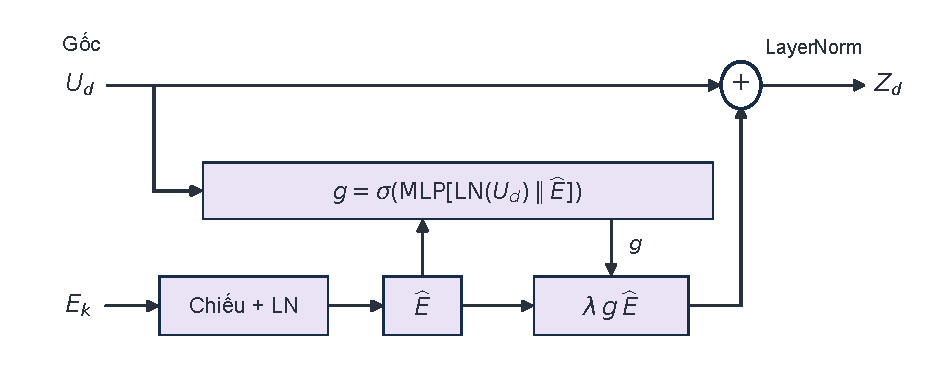
\includegraphics[width=\textwidth]{image/gated-residual-route.pdf}
\caption{Cấu trúc một nhánh phần dư có cổng điều tiết động}
\label{fig:route}
\end{figure}

Tổng hợp lại, biểu diễn của phương thức đích $d$ sau khi nhận các luồng bổ chính tương tác được xác định bởi:
\begin{equation}
 Z_d=\LN_d^{\rm out}\left(
 U_d+\sum_{k\in\mathcal P(d)}\lambda_{k\to d}\,g_{k\to d}\,\widehat E_{k\to d}
 \right),
 \label{eq:ours-residual}
\end{equation}
trong đó $\mathcal P(d)$ là tập hợp các cặp tương tác còn hoạt động hướng tới phương thức đích $d$. Cần nhấn mạnh rằng ba phép chuẩn hóa LayerNorm xuất hiện trong quy trình — tại phép chiếu đích ($\LN_{k\to d}$), tại đầu vào cổng ($\LN_d^{\rm gate}$), và sau tổng phần dư ($\LN_d^{\rm out}$) — là ba tầng chuẩn hóa hoàn toàn độc lập với các tham số riêng biệt \cite{ba2016layernorm}. Sự phân tách này ngăn ngừa hiện tượng dịch chuyển phân phối và kiểm soát chặt chẽ biên độ tín hiệu qua các tầng, giúp việc huấn luyện mô hình luôn duy trì được độ ổn định số học cao. Mức đóng góp thực tế của thông tin tương tác vì vậy phụ thuộc đồng thời vào độ mở của cổng, hệ số $\lambda$ và độ lớn của đặc trưng: khi cổng khép gần về 0, nhánh tương tác gần như bị triệt tiêu để bảo vệ biểu diễn gốc; ngược lại, khi cổng mở gần về 1, tín hiệu tương tác sau khi được điều chỉnh biên độ sẽ hòa nhập tối đa vào dòng chảy đặc trưng của phương thức đích.

\section{Cấu trúc RC-Free}
\label{sec:rcfree-method}

Trong mô hình tích ngoài CP đầy đủ (Full CP), ta xem xét toàn bộ ba cặp tương tác có thể có giữa ba phương thức: MR, MC và RC, dẫn đến việc phải duy trì tới sáu nhánh truyền phần dư có cổng. Tuy nhiên, một câu hỏi kiến trúc mang tính bản chất nảy sinh: \emph{Liệu có nhất thiết phải thiết lập tương tác trực tiếp giữa tất cả các cặp, hay một cấu trúc tinh giản hơn vẫn có thể đạt hiệu quả tương đương, thậm chí vượt trội hơn?}

Xét về bản chất y sinh và hình ảnh học của các nguồn dữ liệu trong bài toán dự báo Alzheimer: ảnh MRI là dữ liệu hình ảnh cấu trúc ba chiều nguyên bản, phản ánh hình thái và mức độ teo thoái hóa của toàn bộ não bộ; các đặc trưng Radiomics là những chỉ số kết cấu định lượng được trích xuất từ chính các vùng não trên ảnh MRI đó; trong khi dữ liệu lâm sàng (Clinical) phản ánh tình trạng nhận thức và hoạt động chức năng toàn diện của người bệnh. Rõ ràng, hình ảnh MRI đóng vai trò như một ``mỏ neo'' thông tin trung tâm, có mối liên hệ mật thiết cả với đặc trưng vi mô của mô não (thông qua Radiomics) lẫn biểu hiện bệnh học vĩ mô (thông qua Clinical). Ngược lại, mối tương tác trực tiếp giữa Radiomics và Clinical (cặp RC) khi không có sự tham chiếu của hình ảnh MRI gốc có thể trở nên dư thừa, hoặc thậm chí tạo ra các tương quan giả (spurious correlations) do nhiễu đo lường trên các thang điểm nhận thức.

Từ nhận định sâu sắc trên, tôi đề xuất kiến trúc \textbf{RC-Free} (loại bỏ cặp tương tác Radiomics--Clinical). Trong thiết kế này, khối tương tác trực tiếp RC được lược bỏ hoàn toàn, đặt biểu diễn hình ảnh MRI làm ``trung tâm kết nối'' cho hai tương tác cốt lõi: MRI--Radiomics (MR) và MRI--Clinical (MC).

Hình~\ref{fig:rcfree-update} trực quan hóa cơ chế truyền thông tin tinh gọn của RC-Free tại một lần khám. Nhìn vào sơ đồ, luồng dữ liệu diễn ra như sau:
\begin{itemize}
\item Cả ba phương thức đầu vào vẫn được duy trì đầy đủ, bảo đảm không làm mất bất kỳ nguồn thông tin nào.
\item Số nhánh truyền phần dư có cổng được tinh giản từ sáu xuống còn bốn nhánh: hình ảnh MRI nhận thông tin bổ chính từ cả hai tương tác MR và MC; đặc trưng Radiomics nhận bổ chính từ MR; và dữ liệu lâm sàng nhận bổ chính từ MC.
\item Radiomics và dữ liệu lâm sàng tuy không tương tác trực tiếp với nhau, nhưng vẫn được liên kết gián tiếp thông qua trung tâm MRI trước khi các biểu diễn được ghép nối thành một vectơ thống nhất.
\end{itemize}

\begin{figure}[H]
\centering
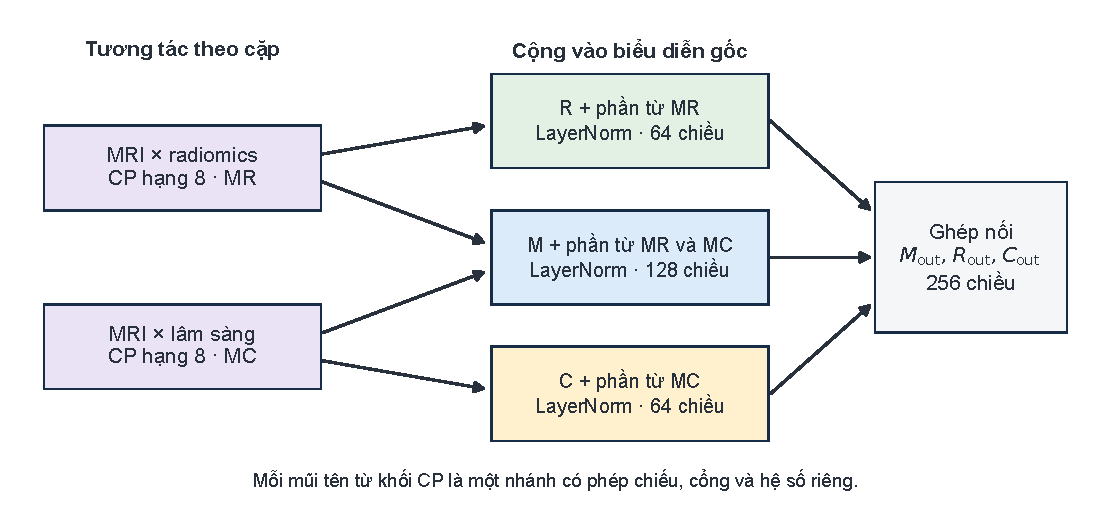
\includegraphics[width=\linewidth]{image/rcfree-update.pdf}
\caption{Bốn nhánh cập nhật đặc trưng trong mô hình RC-Free}
\label{fig:rcfree-update}
\end{figure}

Đặt $D_{k\to d}=\lambda_{k\to d}g_{k\to d}\widehat E_{k\to d}$ là lượng bổ chính tương tác từ cặp $k$ sang phương thức $d$, các phương trình cập nhật đặc trưng trong RC-Free được xác định như sau:
\begin{align}
 M_{\rm out}&=\LN_M^{\rm out}(M+D_{(\mathrm{MR}\to M)}+D_{(\mathrm{MC}\to M)}),\label{eq:rcfree-first}\\
 R_{\rm out}&=\LN_R^{\rm out}(R+D_{(\mathrm{MR}\to R)}),\\
 C_{\rm out}&=\LN_C^{\rm out}(C+D_{(\mathrm{MC}\to C)}).
 \label{eq:rcfree-residual}
\end{align}

Cụ thể, hai khối CP cho MR và MC đều được ấn định hạng $Q=8$. Bốn nhánh truyền tương ứng được kiểm soát bởi bốn phép chiếu theo đích, bốn cổng động độc lập và bốn hệ số điều chỉnh $\lambda$ học được. Sau các phép cộng phần dư và chuẩn hóa LayerNorm, các biểu diễn đầu ra $M_{\rm out}, R_{\rm out}, C_{\rm out}$ lần lượt có kích thước 128, 64 và 64 chiều. Ba vectơ này sau đó được ghép nối liên tiếp thành vectơ đặc trưng đa phương thức $F_t \in \mathbb R^{256}$ tại mỗi lần khám $t$, sẵn sàng làm đầu vào cho khối mô hình hóa chuỗi thời gian tiếp theo. Nhờ việc giữ nguyên kích thước sau ghép nối này, việc chuyển từ Full CP sang RC-Free không làm thay đổi cấu trúc của bất kỳ tầng tính toán nào phía sau, tạo điều kiện thuận lợi để đối chiếu hiệu năng một cách công bằng.

\section{Mô hình thời gian và attention}
\label{sec:temporal-method}

Sau khi đã thu được các vectơ đặc trưng đa phương thức $F_t$ tại từng thời điểm thăm khám, nhiệm vụ tiếp theo là mô hình hóa tiến trình suy giảm bệnh lý theo chiều thời gian. Dự báo tiến triển bệnh Alzheimer đòi hỏi phải khai thác dữ liệu quan sát dọc (longitudinal data). Tuy nhiên, bài toán y sinh thực tế đặt ra hai thách thức lớn mà các kiến trúc học sâu tuần tự thông thường không thể xử lý thỏa đáng:
\begin{enumerate}
\item \emph{Khoảng cách thời gian không đồng đều giữa các lần khám}: Khác với các chuỗi thời gian lý thuyết có chu kỳ đo lường cố định, người bệnh trong các nghiên cứu lâm sàng như ADNI tái khám theo những khoảng thời gian biến thiên thực tế (có khi 6 tháng, có khi 1 năm hoặc lâu hơn). Một mạng LSTM tiêu chuẩn vốn giả định các bước thời gian cách đều nhau, do đó sẽ đánh đồng khoảng cách vài tháng với khoảng cách hàng năm, bỏ qua quy luật bệnh học hiển nhiên: khoảng cách giữa hai lần chụp càng dài thì các biến động tức thời từ lần khám trước càng bị suy giảm và khó dự đoán hơn.

\item \emph{Độ quan trọng không đồng đều giữa các mốc thăm khám}: Các dấu hiệu thoái hóa thần kinh then chốt (như teo hồi hải mã hay tụt dốc điểm nhận thức) không diễn ra dàn trải mà thường bộc lộ rõ nét tại một số thời điểm chuyển giai đoạn nhất định. Do đó, việc chỉ lấy trạng thái ẩn ở bước cuối cùng $h_T$ có thể làm mất mát các tín hiệu cảnh báo sớm ở giai đoạn đầu, trong khi lấy trung bình cộng lại làm loãng các thông tin quan trọng.
\end{enumerate}

Để giải quyết trọn vẹn thách thức thứ nhất, tôi tích hợp mạng Time-Aware LSTM (T-LSTM) \cite{baytas2017patient,aghajanian2025longitudinal}. Nguyên lý cốt lõi của T-LSTM là sử dụng trực tiếp khoảng thời gian thực tế trôi qua giữa hai lần khám để điều chỉnh trạng thái bộ nhớ của mạng. Cụ thể, khoảng thời gian tại lần khám đầu tiên được quy ước bằng không. Tại các lần khám tiếp theo $t \geq 2$, khoảng cách thực tế giữa hai lần chụp liên tiếp $s_t$ và $s_{t-1}$ (tính theo ngày) được quy đổi sang đơn vị năm: $\Delta t_t = (s_t - s_{t-1}) / 365.25$. T-LSTM sử dụng trực tiếp khoảng thời gian này để điều chỉnh trạng thái bộ nhớ mà không cần bổ sung một biểu diễn thời gian được học riêng.

Từ bộ nhớ trước đó $c_{t-1}$, mô hình tách thành phần ngắn hạn $c_{t-1}^{S}$ (chứa các biến động tức thời) và phần còn lại $c_{t-1}^{L}$ (chứa các đặc trưng bệnh lý bền vững), rồi điều chỉnh theo hệ số suy giảm phi tuyến $\gamma_t$:
\begin{align}
 c_{t-1}^{S}&=\tanh(W_Sc_{t-1}+b_S),\qquad
 c_{t-1}^{L}=c_{t-1}-c_{t-1}^{S},\label{eq:tlstm-first}\\
 \gamma_t&=\frac{1}{\log(e+\Delta t_t)},\qquad
 c_{t-1}^{*}=c_{t-1}^{L}+\gamma_t c_{t-1}^{S}.
 \label{eq:tlstm-memory}
\end{align}
Khi $\Delta t_t$ càng lớn, $\gamma_t$ càng giảm, phản ánh chính xác hiện tượng thông tin ngắn hạn từ quá khứ xa bị phai mờ tự nhiên. Bộ nhớ hiệu chỉnh $c_{t-1}^{*}$ này sau đó được đưa vào các cổng cập nhật của LSTM:
\begin{equation}
 c_t=f_t\odot c_{t-1}^{*}+i_t\odot\widetilde c_t,
 \qquad h_t=o_t\odot\tanh(c_t).\label{eq:tlstm-state}
\end{equation}
Trong đó, các cổng đầu vào $i_t$, quên $f_t$, đầu ra $o_t$ và bộ nhớ ứng viên $\widetilde c_t$ được tính từ $F_t$ và $h_{t-1}$ bằng các ánh xạ tuyến tính có hệ số chệch (dùng sigmoid cho các cổng và tanh cho bộ nhớ ứng viên). T-LSTM gồm một lớp một chiều với trạng thái ẩn 128 chiều. Nếu một lần khám được đánh dấu không hợp lệ, mô hình giữ trạng thái trước đó; trong nhóm nghiên cứu này, cả ba lần khám của mỗi người đều hợp lệ.

\begin{figure}[H]
\centering
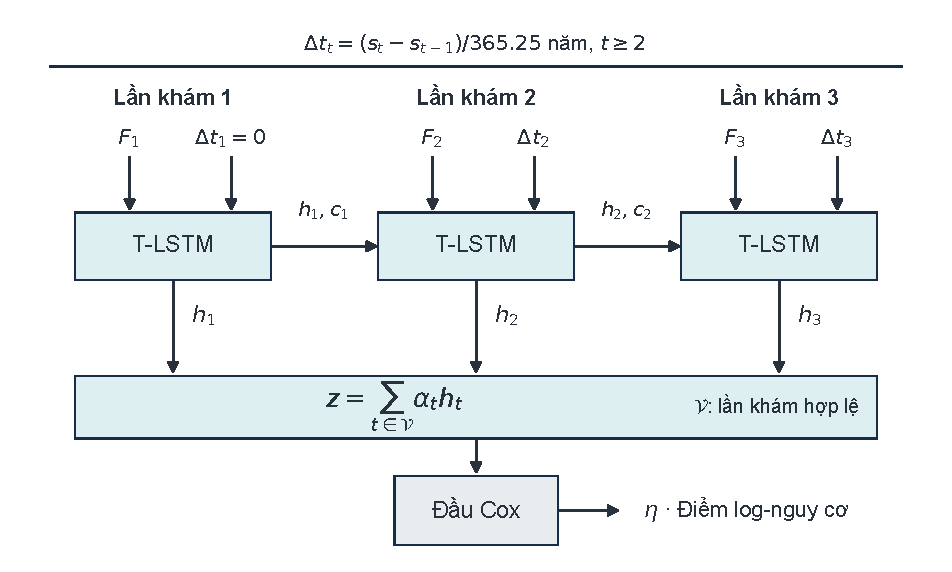
\includegraphics[width=\textwidth]{image/temporal-model.pdf}
\caption{Mô hình thời gian T-LSTM và cơ chế attention}
\label{fig:temporal}
\end{figure}

Để giải quyết thách thức thứ hai, tôi tiếp tục xây dựng một cơ chế Attention cộng theo thời gian (additive temporal attention) \cite{bahdanau2015attention} đặt phía sau T-LSTM, như được minh họa trong Hình~\ref{fig:temporal}. Cơ chế này học cách gán trọng số thích ứng cho từng lần khám:
\begin{equation}
 e_t=v_a^\top\tanh(W_a h_t+b_a),\qquad
 \alpha_t=\frac{\exp(e_t)}{\sum_{j\in\mathcal V}\exp(e_j)},\qquad
 z=\sum_{t\in\mathcal V}\alpha_t h_t.
 \label{eq:temporal-attention}
\end{equation}
Ở đây, $\mathcal V$ là tập hợp các lần khám hợp lệ. Phép chiếu $128\to64\to1$ chấm điểm từng trạng thái ẩn để xác định trọng số $\alpha_t$ của trạng thái đó trong biểu diễn tổng hợp $z\in\mathbb R^{128}$. Sự kết hợp giữa T-LSTM và Attention mang lại một cơ chế mô hình hóa thời gian toàn diện: T-LSTM đảm nhận việc tích lũy và điều tiết dòng chảy lịch sử theo khoảng cách thực tế, còn Attention đảm nhận việc chắt lọc những dấu mốc then chốt để tạo nên biểu diễn chung phục vụ cho bài toán tiên lượng sống còn.

\section{Hàm mục tiêu Cox}
\label{sec:training-method}

Từ biểu diễn chuỗi đã tổng hợp $z$, mục tiêu cuối cùng là dự đoán nguy cơ tiến triển suy giảm nhận thức trong tương lai. Bài toán này không thể giải quyết bằng các hàm mất mát phân loại nhị phân thông thường (như Cross-Entropy), bởi lẽ trong dữ liệu y tế theo dõi dọc, phần lớn người tham gia là dữ liệu kiểm duyệt phải (right-censored) — tức là đến thời điểm nghiên cứu kết thúc hoặc lần tái khám cuối cùng, họ vẫn chưa biểu hiện suy giảm nhận thức. Nếu loại bỏ những bệnh nhân này, mô hình sẽ mắc sai lệch chọn mẫu nghiêm trọng; còn nếu gắn nhãn họ là ``không bệnh'', mô hình sẽ bỏ qua khoảng thời gian họ đã duy trì tình trạng ổn định.

Để giải quyết triệt để bài toán sống còn có kiểm duyệt, tôi đưa biểu diễn $z$ qua một khối mạng perceptron đa tầng tiên lượng gồm lớp tuyến tính $128\to64$, kích hoạt GELU, Dropout 0.30 và lớp tuyến tính $64\to1$ để tính một giá trị log-nguy cơ vô hướng $\eta_i$ cho từng cá thể $i$. Điểm này được đưa trực tiếp vào mô hình nguy cơ tỷ lệ Cox \cite{cox1972regression} mà không qua bất kỳ hàm kích hoạt phi tuyến nào:
\begin{equation}
 h(\tau\mid z_i)=h_0(\tau)\exp(\eta_i),
\end{equation}
trong đó $h(\tau\mid z_i)$ là hàm nguy cơ tức thời tại thời điểm $\tau$, còn $h_0(\tau)$ là hàm nguy cơ nền chung. Theo mô hình này, tại bất kỳ thời điểm nào, người có chỉ số log-nguy cơ $\eta_i$ cao hơn sẽ có nguy cơ tức thời gặp biến cố suy giảm nhận thức lớn hơn theo cấp số mũ.

Hàm mất mát để huấn luyện mạng được xây dựng dựa trên nguyên lý đối log-hợp lý riêng phần (negative partial log-likelihood), xử lý các trường hợp trùng thời điểm biến cố theo quy tắc Breslow \cite{breslow1974covariance} và lấy trung bình trên $N_e$ biến cố quan sát được:
\begin{equation}
 \mathcal L_{\rm Cox}=-\frac{1}{N_e}\sum_k
 \left[\sum_{i\in\mathcal D_k}\eta_i
 -d_k\log\!\left(\sum_{j\in\mathcal R_k}\exp(\eta_j)\right)\right].
 \label{eq:cox-method}
\end{equation}
Ở đây, $\tau_k$ là các mốc thời gian ghi nhận biến cố phân biệt, $\mathcal D_k$ là tập hợp những người xảy ra biến cố tại $\tau_k$ với số lượng $d_k=|\mathcal D_k|$, và $\mathcal R_k=\{j:t_j\geq\tau_k\}$ là tập nguy cơ gồm tất cả những người vẫn đang được theo dõi và chưa gặp biến cố ngay trước thời điểm $\tau_k$.

Ý nghĩa cốt lõi của hàm mất mát Cox nằm ở cơ chế ``so kè thứ tự'': tại mỗi thời điểm một người gặp biến cố, mô hình phạt nặng nếu điểm nguy cơ $\eta_i$ của người đó không vượt trội so với điểm số của tất cả những người khác vẫn đang an toàn trong tập nguy cơ $\mathcal R_k$. Nhờ cơ chế này, ngay cả những người bị kiểm duyệt (không có biến cố) vẫn đóng góp tích cực vào việc huấn luyện mạng bằng cách đóng vai trò làm nhóm chứng so sánh trong tập nguy cơ cho đến tận ngày khám cuối cùng của họ.

Thuật toán~\ref{alg:rcfree-forward} tóm lược toàn bộ luồng tính toán xuôi (forward pass) của mô hình RC-Free từ lúc tiếp nhận ba nguồn dữ liệu thô tại ba lần khám cho đến khi xuất ra điểm log-nguy cơ phục vụ tối ưu hóa hàm mất mát Cox. Các bộ mã hóa và khối hợp nhất dùng chung trọng số qua ba lần khám; bốn nhánh tương tác có cổng được tính từ các biểu diễn trong cùng một lần khám.
\begin{algorithm}[H]
\caption{Luồng tính xuôi của mô hình RC-Free Pairwise Fusion}
\label{alg:rcfree-forward}
\small
\textbf{Đầu vào:} Chuỗi ba lần khám $(t=1,2,3)$ của một cá thể gồm ảnh MRI đã tiền xử lý, vectơ đặc trưng radiomics sau PCA (16 chiều), vectơ lâm sàng kèm chỉ báo quan sát (18 chiều) và khoảng cách thời gian $\Delta t_t$ (với $\Delta t_1=0$).\\
\textbf{Đầu ra:} Điểm log-nguy cơ $\eta\in\mathbb R$ của cá thể.
\begin{enumerate}[leftmargin=1.2em,label=\arabic*.,itemsep=0.2em]
\item Với mỗi lần khám $t=1,2,3$:
\begin{enumerate}[leftmargin=1.2em,label=\alph*.,itemsep=0.15em]
\item Mã hóa ba nguồn đầu vào tại lần khám $t$ thành $M_t\in\mathbb R^{128}$, $R_t\in\mathbb R^{64}$, $C_t\in\mathbb R^{64}$ theo Mục~\ref{sec:preprocessing}; chiếu tuyến tính không hệ số chệch về $\widetilde M_t\in\mathbb R^{32}$, $\widetilde R_t\in\mathbb R^{32}$, $\widetilde C_t\in\mathbb R^{16}$ theo (\ref{eq:input-projection}).
\item Tính đặc trưng tương tác $E_{\mathrm{MR},t}\in\mathbb R^{64}$ từ $(\widetilde M_t,\widetilde R_t)$ và $E_{\mathrm{MC},t}\in\mathbb R^{64}$ từ $(\widetilde M_t,\widetilde C_t)$ bằng hai khối CP hạng $Q=8$ kèm MLP theo (\ref{eq:cp-lowrank})--(\ref{eq:cpblock}); bỏ qua cặp RC.
\item Với mỗi nhánh $k\to d\in\{\mathrm{MR}\to M,\mathrm{MR}\to R,\mathrm{MC}\to M,\mathrm{MC}\to C\}$, tính phép chiếu theo đích $\widehat E_{k\to d,t}$ theo (\ref{eq:target-projection}), cổng điều tiết $g_{k\to d,t}$ theo (\ref{eq:dynamic-gate}) và lượng bổ sung $D_{k\to d,t}=\lambda_{k\to d}\,g_{k\to d,t}\,\widehat E_{k\to d,t}$.
\item Cập nhật phần dư và chuẩn hóa theo (\ref{eq:rcfree-first})--(\ref{eq:rcfree-residual}) để thu được $M_{\mathrm{out},t}\in\mathbb R^{128}$, $R_{\mathrm{out},t}\in\mathbb R^{64}$ và $C_{\mathrm{out},t}\in\mathbb R^{64}$.
\item Ghép nối và ánh xạ thành biểu diễn hợp nhất tại lần khám $t$: $F_t=\operatorname{MLP}_{\mathrm{out}}(M_{\mathrm{out},t}\concat R_{\mathrm{out},t}\concat C_{\mathrm{out},t})\in\mathbb R^{128}$ theo (\ref{eq:concat}).
\end{enumerate}
\item Khởi tạo trạng thái ẩn và bộ nhớ bằng không; đưa chuỗi $(F_t,\Delta t_t)_{t=1}^3$ qua T-LSTM theo (\ref{eq:tlstm-first})--(\ref{eq:tlstm-state}) để thu được các trạng thái ẩn $h_1,h_2,h_3\in\mathbb R^{128}$.
\item Tính trọng số attention $\alpha_t$ và biểu diễn tổng hợp chuỗi $z=\sum_{t=1}^3\alpha_t h_t\in\mathbb R^{128}$ theo (\ref{eq:temporal-attention}).
\item Đưa $z$ qua khối MLP dự báo sống còn Cox ($128\to64\to1$) ở Mục~\ref{sec:training-method} để xuất điểm log-nguy cơ $\eta$.
\end{enumerate}
\end{algorithm}


\section{Đánh giá xếp hạng và phân tầng nguy cơ}
\label{sec:survival-evaluation}

Để kiểm chứng toàn diện giá trị thực tiễn của mô hình RC-Free, việc chỉ nhìn vào một chỉ số đánh giá đơn lẻ là chưa đủ. Một hệ thống học sâu hỗ trợ ra quyết định lâm sàng trong bệnh Alzheimer cần phải trả lời thỏa đáng ba câu hỏi cốt lõi của bác sĩ:
\begin{enumerate}
\item \emph{Khả năng xếp hạng toàn cục}: Liệu mô hình có luôn gán mức nguy cơ cao hơn cho những bệnh nhân sẽ tiến triển suy giảm nhận thức sớm hơn hay không?
\item \emph{Khả năng phân tầng nguy cơ thực tế}: Nếu phân chia bệnh nhân thành hai nhóm nguy cơ cao và thấp, diễn tiến sống còn thực tế của hai nhóm này có tách rời nhau rõ rệt theo thời gian hay không?
\item \emph{Độ chính xác tại các mốc can thiệp cụ thể}: Tại các mốc thời gian lâm sàng then chốt (như 2 năm, 3 năm hay 5 năm), mô hình có khả năng phân biệt chính xác giữa người sẽ gặp biến cố và người duy trì tình trạng ổn định hay không?
\end{enumerate}

Ba câu hỏi này tương ứng với ba lăng kính đánh giá bổ trợ cho nhau: Chỉ số phù hợp Harrell's C-index, phân tích đường cong sống còn Kaplan--Meier, và diện tích dưới đường cong ROC phụ thuộc thời gian (IPCW-AUC), như được hệ thống hóa trong Hình~\ref{fig:evaluation-map}. Toàn bộ các đánh giá này được thực hiện trực tiếp trên điểm nguy cơ dự đoán từ ba mô hình RC-Free độc lập (tương ứng với ba lần khởi tạo ngẫu nhiên) mà không hề trải qua bất kỳ bước huấn luyện lại hay tinh chỉnh siêu tham số nào, bảo đảm tính khách quan tuyệt đối.

\begin{figure}[H]
\centering
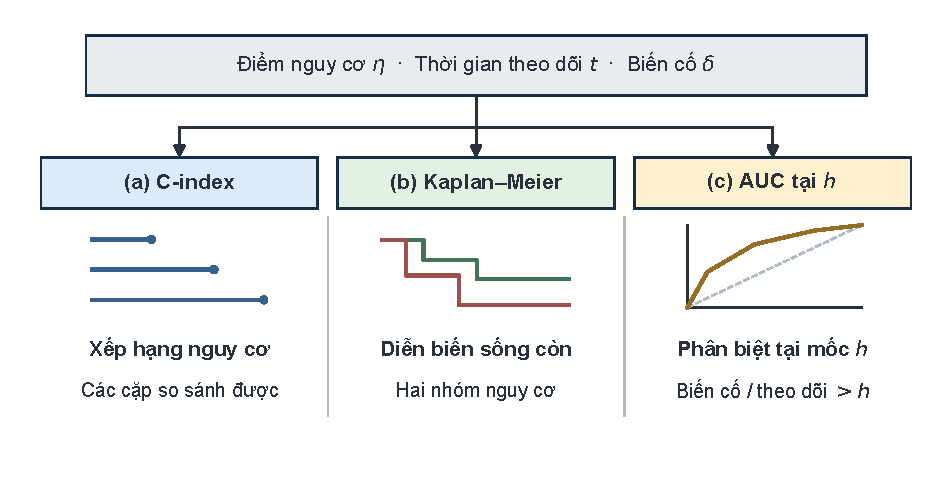
\includegraphics[width=\textwidth]{image/evaluation-map.pdf}
\caption{Ba góc nhìn đánh giá và phân tầng điểm nguy cơ sống còn}
\label{fig:evaluation-map}
\end{figure}

\subsection{C-index}
Chỉ số phù hợp C-index (Concordance Index) theo quy ước Harrell \cite{harrell1996multivariable} là thước đo chuẩn mực nhất để đánh giá năng lực xếp hạng của mô hình sống còn trên toàn bộ dải thời gian theo dõi. Về mặt trực giác, C-index đo lường xác suất mà thứ tự nguy cơ do mô hình dự đoán đồng thuận với thứ tự xảy ra biến cố thực tế giữa hai bệnh nhân bất kỳ.

Cụ thể, xét tất cả các cặp cá thể $(i,j)$ thỏa mãn điều kiện có thể so sánh được: người thứ nhất có biến cố ($\delta_i=1$) và thời điểm biến cố của người đó diễn ra trước thời điểm kết thúc theo dõi của người thứ hai ($t_i<t_j$). Nếu mô hình dự báo chính xác rằng người gặp biến cố sớm hơn có điểm nguy cơ cao hơn ($\eta_i>\eta_j$), cặp đó được chấm 1 điểm đồng thuận. Trường hợp mô hình dự đoán hai người có cùng điểm nguy cơ ($\eta_i=\eta_j$), cặp đó được chấm 0.5 điểm. Ngược lại, nếu thứ tự dự báo bị đảo ngược ($\eta_i<\eta_j$), cặp đó nhận 0 điểm. Các cặp có thời gian theo dõi bằng nhau hoặc cả hai cùng bị kiểm duyệt không thể xác định thứ tự nên không được đưa vào so sánh. C-index bằng 0.5 tương đương với mức đoán ngẫu nhiên, trong khi 1.0 đại diện cho khả năng phân biệt hoàn hảo. Kết quả C-index qua ba lần khởi tạo được báo cáo dưới dạng trung bình $\pm$ độ lệch chuẩn mẫu (SD, mẫu số $n-1$) nhằm phản ánh độ ổn định của kiến trúc trước biến thiên ngẫu nhiên của trọng số ban đầu.

\subsection{Kaplan--Meier và nhóm nguy cơ đồng thuận}
Trong thực hành y khoa, các chỉ số điểm số liên tục cần được chuyển hóa thành các phân tầng nguy cơ rõ ràng để hỗ trợ bác sĩ phân loại bệnh nhân và đưa ra phác đồ theo dõi thích hợp. Để thực hiện việc này một cách hoàn toàn khách quan và không chịu thiên lệch từ tập kiểm tra, tôi sử dụng trung vị của điểm nguy cơ $\eta$ trên tập huấn luyện làm ngưỡng phân nhóm. Người có điểm nguy cơ vượt trên ngưỡng trung vị được xếp vào nhóm nguy cơ cao, trong khi những người có điểm bằng hoặc thấp hơn ngưỡng thuộc nhóm nguy cơ thấp.

Tuy nhiên, việc phân nhóm chỉ dựa trên một mô hình đơn lẻ có thể chịu ảnh hưởng bởi tính ngẫu nhiên của lần khởi tạo đó. Do đó, tôi áp dụng \emph{nguyên tắc đồng thuận đa số} (majority voting): một người tham gia được xếp vào nhóm nguy cơ cao (hoặc thấp) nếu có ít nhất hai trong ba lần khởi tạo cùng phân loại người đó vào nhóm này. 

Sau khi xác lập nhóm đồng thuận, đường cong Kaplan--Meier (KM) \cite{kaplan1958nonparametric} được sử dụng để ước lượng xác suất chưa ghi nhận biến cố suy giảm nhận thức theo thời gian ở từng nhóm. Hai đường cong được trình bày kèm theo dải khoảng tin cậy (CI) 95\%, các dấu kiểm duyệt tại thời điểm rời theo dõi, cùng bảng số lượng người còn nguy cơ (number at risk) ngay trước các mốc 0, 2, 3 và 5 năm. Sự khác biệt giữa hai đường cong được kiểm định chặt chẽ bằng kiểm định log-rank để xác định ý nghĩa thống kê. Đồng thời, một mô hình hồi quy Cox đơn biến được áp dụng trên nhãn phân nhóm để định lượng tỷ số nguy cơ (Hazard Ratio - HR) cùng khoảng tin cậy 95\%, cho biết người thuộc nhóm nguy cơ cao có tốc độ gặp biến cố gấp bao nhiêu lần so với nhóm nguy cơ thấp. Giả định nguy cơ tỷ lệ được kiểm tra cẩn trọng thông qua phần dư Schoenfeld với thời gian được biến đổi theo thứ hạng. Mặc dù đồ thị chỉ thể hiện năm năm đầu nhằm tập trung vào giai đoạn can thiệp sớm, kiểm định log-rank và ước lượng HR sử dụng trọn vẹn toàn bộ thời gian theo dõi.

\subsection{AUC theo thời gian tại 2, 3 và 5 năm}
Bên cạnh khả năng xếp hạng toàn cục của C-index, các bác sĩ thường đối mặt với các câu hỏi tiên lượng cụ thể tại những cửa sổ thời gian xác định: ``Liệu bệnh nhân này có tiến triển trong vòng 2 năm tới hay không? 3 năm? hay 5 năm?''. Để trả lời chính xác câu hỏi này, tôi sử dụng diện tích dưới đường cong ROC phụ thuộc thời gian (time-dependent cumulative/dynamic AUC).

Tại mỗi mốc thời gian đánh giá $h \in \{2, 3, 5\text{ năm}\}$, tập bệnh nhân được phân chia thành hai nhóm: nhóm biến cố $\mathcal C_h=\{i:\delta_i=1,t_i\leq h\}$ gồm những người đã thực sự suy giảm nhận thức trước hoặc tại mốc $h$; và nhóm đối chứng $\mathcal D_h=\{j:t_j>h\}$ gồm những người vẫn duy trì tình trạng ổn định sau mốc $h$. Thách thức toán học lớn nhất ở đây là hiện tượng kiểm duyệt: những người bị kiểm duyệt trước thời điểm $h$ không thể biết chắc chắn tình trạng bệnh lý tại $h$, do đó không thể gán vào nhóm nào. Nếu đơn thuần loại bỏ những người này, mẫu đánh giá sẽ bị sai lệch nghiêm trọng.

Để giải quyết bài toán kiểm duyệt một cách chuẩn xác, tôi áp dụng phương pháp gán trọng số nghịch đảo xác suất kiểm duyệt (Inverse Probability of Censoring Weighting - IPCW) \cite{polsterl2020scikit,hung2010time}. Trọng số IPCW bù đắp xác suất bị mất dấu bằng cách gán trọng số $w_i = 1/\widehat G(t_i)$ cho mỗi ca biến cố quan sát được, trong đó hàm phân phối kiểm duyệt $\widehat G(u)$ được ước lượng từ tập huấn luyện thông qua đường Kaplan--Meier cho biến cố kiểm duyệt. Công thức ước lượng AUC tích lũy/động có dạng:
\begin{equation}
 \widehat{\operatorname{AUC}}(h)=
 \frac{\displaystyle\sum_{i\in\mathcal C_h}w_i
 \sum_{j\in\mathcal D_h}\kappa(\eta_i,\eta_j)}
 {\displaystyle |\mathcal D_h|\sum_{i\in\mathcal C_h}w_i},
 \qquad
 \kappa(a,b)=\begin{cases}
 1,&a>b,\\
 \tfrac12,&a=b,\\
 0,&a<b.
 \end{cases}
 \label{eq:ipcw-auc}
\end{equation}
Ý nghĩa của Công thức~\eqref{eq:ipcw-auc} là tính toán tỷ lệ các cặp (biến cố, đối chứng) mà mô hình xếp hạng đúng, có điều chỉnh trọng số để đại diện cho toàn bộ quần thể ban đầu. Khi triển khai tính toán bằng thư viện \texttt{scikit-survival}, các điểm nguy cơ kề nhau chênh lệch dưới $10^{-8}$ được coi là đồng điểm. Đồng thời, để tránh nguy cơ ngoại suy phân phối kiểm duyệt khi thời gian theo dõi tối đa ở tập xác thực (18.26 năm) vượt quá tập huấn luyện (13.95 năm), quy trình áp dụng kỹ thuật chặn thời gian theo dõi tại ngưỡng $h+\varepsilon$ (với $\varepsilon$ được xác định chính xác qua hàm \texttt{nextafter}). 

Tổng kết lại, bộ ba chỉ số C-index, Kaplan--Meier và IPCW-AUC tạo nên một khung đánh giá toàn diện và khắt khe, kiểm chứng vững chắc năng lực của mô hình RC-Free từ góc độ lý thuyết xếp hạng đến ứng dụng phân tầng nguy cơ thực tiễn trong y khoa. Toàn bộ các kết quả thực nghiệm chi tiết sẽ được trình bày và phân tích có hệ thống trong Chương~\ref{chap:results}.

\FloatBarrier

\chapter[Thực nghiệm, kết quả và phân tích]{Thực nghiệm,\\kết quả và phân tích}
\label{chap:results}

Chương này kiểm chứng từng bước thiết kế của Chương~\ref{chap:method} theo đúng trình tự năm câu hỏi nghiên cứu ở Bảng~\ref{tab:rq}. Thay vì đưa ngay mô hình cuối cùng, các thí nghiệm được trình bày từ đơn giản đến hoàn chỉnh: (1) dữ liệu dọc và đa phương thức có giúp ích không (RQ1--RQ2); (2) tương tác song tuyến theo cặp có vượt ghép nối không (RQ3); (3) phân rã CP nén được bao nhiêu tham số và việc bỏ cặp RC có hợp lý không khi đặt cạnh bảy tổ hợp cặp cùng quy trình tham chiếu (RQ4--RQ5); và cuối cùng (4) kiểm chứng khả năng phân tầng sống còn thực tế của RC-Free qua AUC theo thời gian và đường cong Kaplan--Meier.

\section{Thiết lập huấn luyện và diễn biến hội tụ}
\label{sec:experimental-protocol}
Mọi thí nghiệm sử dụng cùng cách chia cố định theo mã người tham gia đã trình bày ở Mục~\ref{sec:data-split} (251 huấn luyện / 54 xác thực / 54 kiểm tra hậu nghiệm; tương ứng 74 / 16 / 16 biến cố), trong đó các tham số tiền xử lý chỉ khớp trên tập huấn luyện. Tập xác thực có 480 cặp so sánh hợp lệ và tập kiểm tra hậu nghiệm có 528 cặp. Loạt thăm dò đầu vào (RQ1--RQ2) chạy một lần khởi tạo; toàn bộ các so sánh kiến trúc chính và đánh giá sống còn chạy qua ba mã khởi tạo ngẫu nhiên (seed 20260727, 20260728 và 20260729), báo cáo trung bình $\pm$ độ lệch chuẩn mẫu (SD).

Do ảnh MRI 3D chiếm nhiều bộ nhớ GPU trong khi hàm mất mát Cox nhạy với cỡ lô nhỏ, quy trình huấn luyện được thiết lập như sau:
\begin{enumerate}
\item \emph{Tối ưu hóa}: Dùng AdamW \cite{loshchilov2019adamw} với tốc độ học ban đầu $10^{-4}$, weight decay $10^{-4}$, $(\beta_1,\beta_2)=(0.9,0.999)$ và cắt chuẩn gradient ở ngưỡng $1.0$ \cite{pascanu2013difficulty}.
\item \emph{Cỡ lô, tích lũy gradient và độ chính xác hỗn hợp}: Đặt cỡ lô bằng 6 người và tích lũy gradient qua 2 lô trước mỗi bước cập nhật trọng số (tập nguy cơ Cox tính riêng trên từng lô). Huấn luyện dùng FP16 \cite{micikevicius2018mixed} để giảm bộ nhớ, riêng phép tính log-sum-exp trong hàm mất mát Cox ép về FP32 để giữ ổn định số học.
\item \emph{Lấy mẫu lô hợp lệ cho Cox}: Bộ lấy mẫu phân bổ sao cho mỗi người xuất hiện đúng một lần trong mỗi vòng (42 lô/vòng) và mỗi lô luôn có ít nhất một cặp so sánh hợp lệ. Qua cả ba lần khởi tạo, toàn bộ 4032 lô huấn luyện đều hợp lệ.
\item \emph{Điều chỉnh tốc độ học và chọn mô hình}: Huấn luyện tối đa 100 vòng với \texttt{ReduceLROnPlateau} \cite{pytorchReduceLROnPlateau} theo dõi hàm mất mát Cox xác thực (giảm một nửa tốc độ học sau 5 vòng không cải thiện, mức sàn $10^{-6}$). Sau 10 vòng khởi động, dừng sớm theo dõi C-index xác thực (ngưỡng cải thiện tối thiểu 0.002, chờ 20 vòng); mô hình lưu lại là checkpoint có C-index xác thực cao nhất.
\end{enumerate}

\begin{figure}[H]
\centering
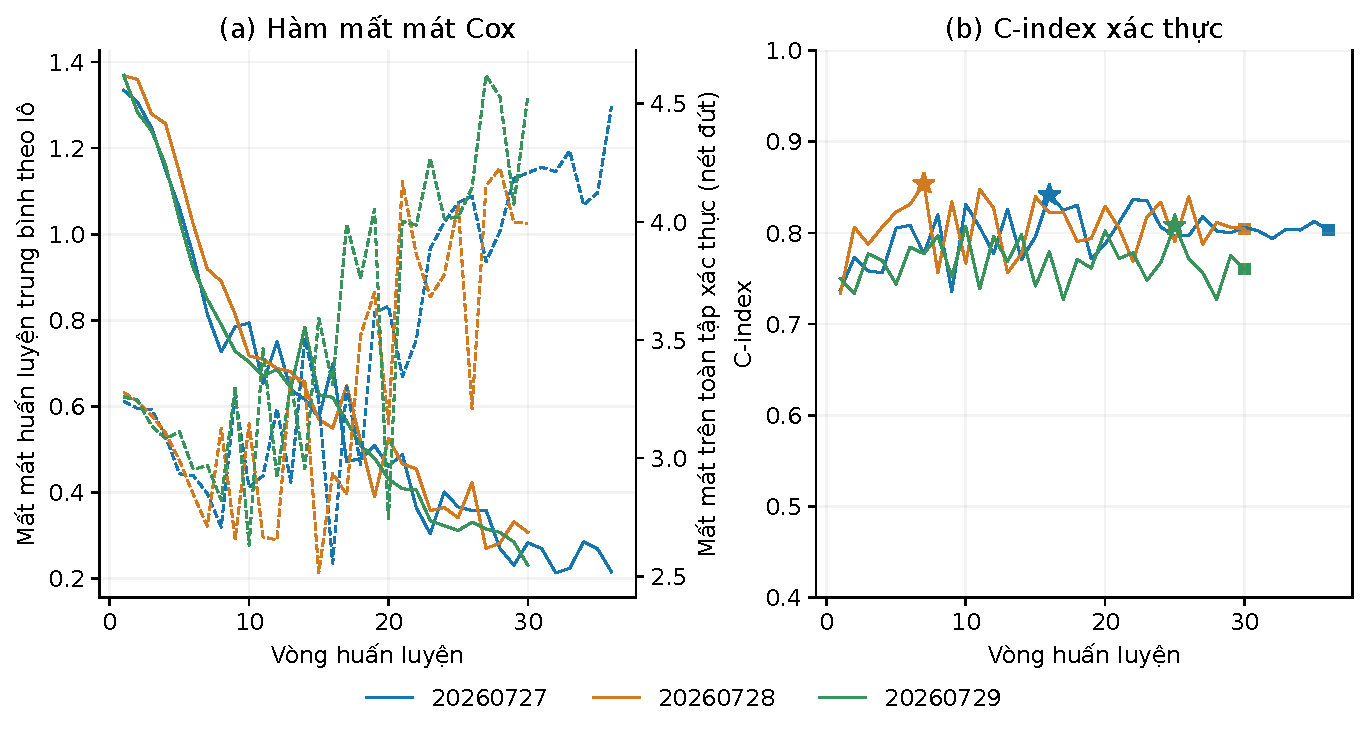
\includegraphics[width=\textwidth]{image/empirical-training.pdf}
\caption{Diễn biến huấn luyện của mô hình RC-Free qua ba lần khởi tạo}
\label{fig:empirical-training}
\captionsetup{justification=raggedright}
\caption*{Ô (a): hàm mất mát huấn luyện trung bình theo lô (đường liền, trục trái) và hàm mất mát xác thực trên toàn tập (đường đứt, trục phải). Ô (b): C-index xác thực theo từng vòng; dấu sao là mô hình được chọn, hình vuông là vòng dừng sớm.}
\end{figure}

Hình~\ref{fig:empirical-training} cho thấy trong cả ba lần chạy, hàm mất mát huấn luyện giảm đều (từ 1.33--1.37 xuống 0.22--0.31) trong khi hàm mất mát xác thực có xu hướng tăng dần (từ 3.24--3.28 lên 3.99--4.53), gợi ý hiện tượng quá khớp khi tiếp tục huấn luyện trên mẫu nhỏ. Lưu ý rằng không nên so trực tiếp trị số tuyệt đối giữa hai trục mất mát vì độ lớn hàm mất mát Cox phụ thuộc vào kích thước tập nguy cơ \cite{kvamme2019time} (tối đa 6 người mỗi lô huấn luyện so với cả 54 người trên tập xác thực). Vì mục tiêu của bài toán là xếp hạng nguy cơ, tôi chọn mô hình theo đỉnh C-index xác thực (ô b): ba lượt chạy lần lượt chọn checkpoint tại các vòng 16, 7 và 25 (đạt C-index xác thực 0.8417, 0.8542 và 0.8083) và dừng sớm ở các vòng 36, 30 và 30.

\section{Vai trò của dữ liệu dọc và đa phương thức (RQ1--RQ2)}
Bước đầu tiên của thực nghiệm kiểm tra xem việc thêm thông tin theo thời gian (nhiều lần chụp MRI) và thêm hai nguồn radiomics, lâm sàng có thực sự nâng cao khả năng xếp hạng nguy cơ hay không. Bảng~\ref{tab:exploratory} tổng hợp kết quả loạt thăm dò trên tập xác thực (seed 20260727).

\begin{table}[H]
\centering\small
\caption[So sánh cấu hình đầu vào cho RQ1--RQ2]{C-index xác thực của các cấu hình đầu vào tăng dần (seed 20260727).}
\label{tab:exploratory}
\begin{tabularx}{\linewidth}{@{}Y r@{}}
\toprule
\textbf{Cấu hình mô hình} & \textbf{C-index $\uparrow$} \\
\midrule
MRI cuối (đơn thời điểm) & 0.7333 \\
MRI dọc và T-LSTM & 0.7333 \\
MRI dọc, T-LSTM và attention & 0.7833 \\
Ghép nối ba nguồn dữ liệu (MRI + Radiomics + Lâm sàng) & \textbf{0.8125} \\
\bottomrule
\end{tabularx}
\end{table}

Kết quả cho thấy hai bước nhảy rõ rệt. Thứ nhất, chỉ dùng trạng thái cuối của T-LSTM trên ba ảnh MRI chưa vượt được mô hình chỉ dùng ảnh cuối (cùng 0.7333), nhưng khi bổ sung cơ chế attention để tổng hợp có trọng số cả ba lần khám, C-index tăng từ 0.7333 lên 0.7833 (+0.0500). Điều này cho thấy giá trị của dữ liệu dọc chỉ phát huy rõ khi mô hình được quyền cân đối đóng góp giữa các lần chụp thay vì chỉ dựa vào bước cuối. Thứ hai, khi bổ sung radiomics và dữ liệu lâm sàng bằng phép ghép nối đơn giản, C-index tăng tiếp lên \textbf{0.8125} (+0.0292 so với cấu hình chỉ dùng MRI tốt nhất). Từ cơ sở này, toàn bộ các thí nghiệm tiếp theo giữ đồng thời cả ba nguồn dữ liệu cùng T-LSTM và attention.

\section{Đối chiếu ghép nối và tương tác tích ngoài (RQ3)}
\label{sec:matched-fusion}
Khi đã giữ đủ ba nguồn đầu vào, câu hỏi tiếp theo là liệu mô hình hóa tương tác song tuyến bằng phép tích ngoài có hiệu quả hơn ghép nối đặc trưng hay không. Để cô lập đúng tác động của lớp hợp nhất, tôi cố định toàn bộ các khối còn lại (ResNet-18 3D, T-LSTM ẩn 128, attention, hàm mất mát Cox Breslow và cấu hình huấn luyện) và khởi tạo \emph{cùng trọng số ban đầu} cho các phần chung ở mỗi lần chạy (Bảng~\ref{tab:matched-fusion}).

\begin{table}[H]
\centering\small
\caption[So sánh ghép nối và tích ngoài]{C-index xác thực của ghép nối và tích ngoài khi giữ cùng trọng số khởi tạo cho các phần chung (trung bình $\pm$ SD qua ba lần chạy).}
\label{tab:matched-fusion}
\begin{tabularx}{\linewidth}{@{}Y r@{}}
\toprule
\textbf{Cấu trúc hợp nhất} & \textbf{C-index $\uparrow$} \\
\midrule
Concatenation (ghép nối) & $0.8149\pm0.0214$ \\
Full Outer-Product (tích ngoài đầy đủ) & $\mathbf{0.8285\pm0.0272}$ \\
\bottomrule
\end{tabularx}
\end{table}

Trong cùng điều kiện khởi tạo, Full Outer-Product đạt C-index xác thực trung bình \textbf{0.8285}, cao hơn mức 0.8149 của ghép nối (chênh lệch trung bình \textbf{0.0135} tính trên giá trị chưa làm tròn). Mức cải thiện này cho thấy việc biểu diễn tường minh các tích chéo giúp khai thác tốt hơn mối liên hệ giữa ba nguồn dữ liệu, tạo cơ sở để lấy Full Outer-Product làm mốc xuất phát cho hai bước tinh giản tiếp theo: nén tham số bằng phân rã CP và lược bỏ cặp tương tác dư thừa.

\section{Phân rã CP, RC-Free và đối chiếu (RQ4--RQ5)}
\label{sec:cp-results}
\label{sec:ablation-results}
\label{sec:rcfree-multiseed}
\label{sec:standardized-benchmark}
\label{sec:paper-adaptation-results}

Từ cấu trúc Full Outer-Product, tôi tiến hành hai bước đơn giản hóa nối tiếp nhau trên cùng bộ ba seed (20260727--20260729), rồi đặt mô hình chọn được cạnh quy trình tham chiếu CNN--PCA--T-LSTM.

\subsection{Mức giảm tham số nhờ phân rã CP (RQ4)}
\label{sec:computational-efficiency}
Khi chuyển từ Full Outer-Product sang Full CP, toàn bộ các bộ mã hóa, nhánh phần dư có cổng và khối thời gian được giữ nguyên; chỉ lớp song tuyến đầu của ba cặp MR, MC và RC được tham số hóa bằng CP với hạng lần lượt là 8, 8 và 4 (Bảng~\ref{tab:cpconfig}). Bảng~\ref{tab:interaction-parameters} đối chiếu số tham số ở ba phạm vi tính khác nhau.

\begin{table}[H]
\centering\small
\caption[Tham số tương tác và toàn mạng]{Số tham số của Full Outer-Product và Full CP ở ba phạm vi (gồm độ chệch).}
\label{tab:interaction-parameters}
\begin{tabularx}{\linewidth}{@{}Y r r@{}}
\toprule
\textbf{Phạm vi} & \textbf{Full Outer-Product} & \textbf{Full CP} \\
\midrule
Ba lớp song tuyến đầu & 229696 & \textbf{3712} \\
Ba khối tương tác, gồm MLP & 248608 & \textbf{22624} \\
Toàn mạng & 33760941 & \textbf{33534957} \\
\bottomrule
\end{tabularx}
\end{table}

Bảng~\ref{tab:interaction-parameters} cho thấy rõ bản chất của việc nén tham số bằng CP: ở đúng ba lớp song tuyến đầu, số tham số giảm từ 229696 xuống còn 3712, tức \textbf{giảm 98.38\%}; tính cả phần MLP phía sau của ba khối tương tác, mức giảm vẫn là \textbf{90.90\%}. Ngược lại, trên quy mô toàn mạng, mức giảm chỉ đạt khoảng 0.67\% vì xương sống ResNet-18 3D của nhánh ảnh MRI chiếm phần lớn số tham số và không thay đổi. Đổi lại mức tinh giản mạnh ở lớp tương tác, C-index xác thực trung bình của Full CP (0.8278) thấp hơn Full Outer-Product (0.8344) khoảng 0.0066 trên loạt so sánh chính (Bảng~\ref{tab:standard-bench}). Thay vì dừng ở Full CP, bước tiếp theo kiểm tra xem việc loại bỏ bớt cặp tương tác dư thừa có vừa giảm thêm tham số vừa lấy lại C-index hay không.

\subsection{So sánh bảy cấu trúc tương tác cặp và lựa chọn RC-Free (RQ5)}
\label{sec:new-topology}
Để kiểm chứng giả thuyết rằng không cần giữ đủ cả ba cặp tương tác, tôi khảo sát toàn bộ bảy tổ hợp CP có ít nhất một cặp (ba cấu hình 1 cặp, ba cấu hình 2 cặp và Full CP 3 cặp). Điểm quan trọng là \emph{mọi cấu trúc đều giữ đủ cả ba nguồn đầu vào cùng đường truyền gốc của chúng}; khác biệt duy nhất là những cặp tương tác nào được bật. Bảng~\ref{tab:new-topology} báo cáo kết quả qua ba lần khởi tạo.

\begin{table}[H]
\centering\small
\caption[So sánh bảy cấu trúc có tương tác cặp]{Số tham số toàn mạng và C-index xác thực của bảy cấu trúc CP có tương tác cặp (trung bình $\pm$ SD qua ba lần khởi tạo).}
\label{tab:new-topology}
\begin{tabularx}{\linewidth}{@{}Y c r r@{}}
\toprule
\textbf{Cấu trúc} & \textbf{Cặp / nhánh} & \textbf{Số tham số} & \textbf{C-index $\uparrow$} \\
\midrule
MR-only & 1 / 2 & 33484165 & $0.8299\pm0.0267$ \\
MC-only & 1 / 2 & 33484037 & $0.8236\pm0.0237$ \\
RC-only & 1 / 2 & 33464165 & $0.8319\pm0.0214$ \\
RC-Free (MR+MC) & 2 / 4 & 33519497 & $\mathbf{0.8347\pm0.0237}$ \\
MR-Free (MC+RC) & 2 / 4 & 33499625 & $0.8243\pm0.0249$ \\
MC-Free (MR+RC) & 2 / 4 & 33499753 & $0.8222\pm0.0156$ \\
Full CP & 3 / 6 & 33534957 & $0.8278\pm0.0250$ \\
\bottomrule
\end{tabularx}
\end{table}

Trong bảy cấu trúc, \textbf{RC-Free (MR+MC)} đạt C-index xác thực trung bình cao nhất (\textbf{0.8347}), đứng thứ hai là RC-only (0.8319). So với Full CP, bỏ cặp RC giúp giảm số nhánh phần dư từ sáu xuống bốn, \textbf{tiết kiệm 15460 tham số} và nâng C-index trung bình từ 0.8278 lên 0.8347. Xét đồng thời cả tiêu chí giữ tương tác tường minh quanh ảnh MRI lẫn hiệu quả xếp hạng và độ tinh gọn, RC-Free là lựa chọn hợp lý nhất để đưa vào phân tích sống còn.

\subsection{Đối chiếu tổng thể với quy trình tham chiếu}
Bảng~\ref{tab:standard-bench} đặt RC-Free cạnh Full Outer-Product, Full CP và bản tái lập có điều chỉnh quy trình CNN--PCA--T-LSTM của Aghajanian và cộng sự trên cùng tập xác thực.

\begin{table}[H]
\centering\small
\caption[So sánh C-index và độ phức tạp mô hình]{C-index xác thực dưới dạng trung bình $\pm$ SD qua ba lần khởi tạo. M biểu thị triệu tham số.}
\label{tab:standard-bench}
\begin{tabularx}{\linewidth}{@{}Y r r c@{}}
\toprule
\textbf{Mô hình} & \textbf{C-index $\uparrow$} & \textbf{Tham số (M)} & \textbf{Cặp/nhánh} \\
\midrule
CNN--PCA--T-LSTM (thích nghi) & $0.7417\pm0.0693$ & $33.20\text{--}33.21$ & 0 / 0 \\
Full Outer-Product (loạt chính) & $0.8344\pm0.0148$ & $33.76$ & 3 / 6 \\
Full CP Pairwise & $0.8278\pm0.0250$ & $33.53$ & 3 / 6 \\
RC-Free Pairwise & $0.8347\pm0.0237$ & $33.52$ & 2 / 4 \\
RC-Free Fixed-$\lambda$ & $0.8347\pm0.0313$ & $33.52$ & 2 / 4 \\
\bottomrule
\end{tabularx}
\end{table}


So với Full Outer-Product, RC-Free \textbf{giảm 241444 tham số} (rút từ 3 cặp / 6 nhánh xuống 2 cặp / 4 nhánh) trong khi vẫn đạt C-index trung bình cao nhất (\textbf{0.8347} so với 0.8344). Đặt cạnh quy trình tham chiếu CNN--PCA--T-LSTM ($0.7417\pm0.0693$), cả ba kiến trúc hợp nhất đa phương thức đầu-cuối đều đạt C-index cao hơn khoảng 0.086--0.093 điểm, đồng thời có độ lệch chuẩn qua ba lần khởi tạo nhỏ hơn gần ba lần (0.0148--0.0250 so với 0.0693). Kết quả này cho thấy quy trình huấn luyện đầu-cuối kết hợp bộ mã hóa tiền huấn luyện và tương tác đa nguồn mang lại cả độ chính xác xếp hạng lẫn độ ổn định vượt trội so với quy trình hai bước chỉ dùng đặc trưng ảnh nén qua PCA.

\section{Phân tích sống còn của RC-Free}
\label{sec:posthoc-test}
\label{sec:survival-results}
Với cấu trúc RC-Free đã chọn, phần này kiểm chứng chất lượng điểm nguy cơ $\eta_i$ trên cả tập xác thực (đánh giá chính) và tập kiểm tra hậu nghiệm theo hai góc nhìn: phân biệt tại từng thời hạn (IPCW-AUC) và phân tầng nhóm nguy cơ theo thời gian (Kaplan--Meier).

\subsection{C-index và AUC theo thời gian tại 2, 3 và 5 năm}
Bảng~\ref{tab:survival-metrics} tóm tắt C-index cùng AUC tại ba mốc thời gian, đi kèm Bảng~\ref{tab:horizon-support} báo cáo số ca biến cố, số đối chứng và số ca kiểm duyệt tại từng mốc nhằm làm rõ cơ sở mẫu của từng ước lượng.

\begin{table}[H]
\centering\small
\caption[C-index và AUC của RC-Free]{C-index và AUC của RC-Free, trình bày dưới dạng trung bình $\pm$ SD qua ba lần khởi tạo. Mỗi tập gồm 54 người với 16 biến cố.}
\label{tab:survival-metrics}
\begin{tabularx}{\linewidth}{@{}Y r r@{}}
\toprule
\textbf{Chỉ số} & \textbf{Xác thực (chính)} & \textbf{Kiểm tra (hậu nghiệm)} \\
\midrule
C-index & $\mathbf{0.8347\pm0.0237}$ & $\mathbf{0.8466\pm0.0267}$ \\
AUC 2 năm & $\mathbf{0.9805\pm0.0149}$ & $0.8858\pm0.0245$ \\
AUC 3 năm & $\mathbf{0.9788\pm0.0162}$ & $0.8770\pm0.0318$ \\
AUC 5 năm & $0.7889\pm0.0632$ & $0.8483\pm0.0508$ \\
\bottomrule
\end{tabularx}
\end{table}

\begin{table}[H]
\centering\small
\caption[Số người theo trạng thái và xác suất chưa kiểm duyệt tại từng mốc]{Số người có biến cố / theo dõi quá mốc / kiểm duyệt trước hoặc tại mốc; $\widehat G(h)$ ước lượng từ tập huấn luyện.}
\label{tab:horizon-support}
\begin{tabularx}{\linewidth}{@{}c Y Y r@{}}
\toprule
\textbf{Năm} & \textbf{Xác thực} & \textbf{Kiểm tra hậu nghiệm} & \textbf{$\widehat G(h)$} \\
\midrule
2 & 7 / 37 / 10 & 8 / 37 / 9 & $0.831$ \\
3 & 7 / 34 / 13 & 11 / 29 / 14 & $0.697$ \\
5 & 12 / 19 / 23 & 14 / 16 / 24 & $0.475$ \\
\bottomrule
\end{tabularx}
\end{table}


Trên tập xác thực, RC-Free đạt AUC cao ở các mốc gần (\textbf{0.9805} tại 2 năm và \textbf{0.9788} tại 3 năm) rồi giảm xuống 0.7889 tại mốc 5 năm. Khi đối chiếu với Bảng~\ref{tab:horizon-support}, sự thay đổi này gắn với cấu trúc mẫu tại từng mốc. Tại mốc 2 và 3 năm, tập xác thực chỉ có \textbf{7 biến cố tích lũy}, nên độ biến động trên mẫu nhỏ là đáng kể. Đến mốc 5 năm, dù số biến cố tăng lên 12, số người còn được theo dõi quá 5 năm giảm từ 37 xuống còn 19 do 23 người bị kiểm duyệt. Hình~\ref{fig:empirical-roc} phản ánh rõ hiện tượng này: ở mốc 5 năm trên tập xác thực, các đường ROC giữa ba seed phân tán rộng hơn (SD tăng lên 0.0632) so với hai mốc đầu. Trên tập kiểm tra hậu nghiệm, kết quả ổn định hơn qua cả ba mốc (0.8858, 0.8770 và 0.8483) với C-index đạt $0.8466\pm0.0267$.

\begin{figure}[H]
\centering
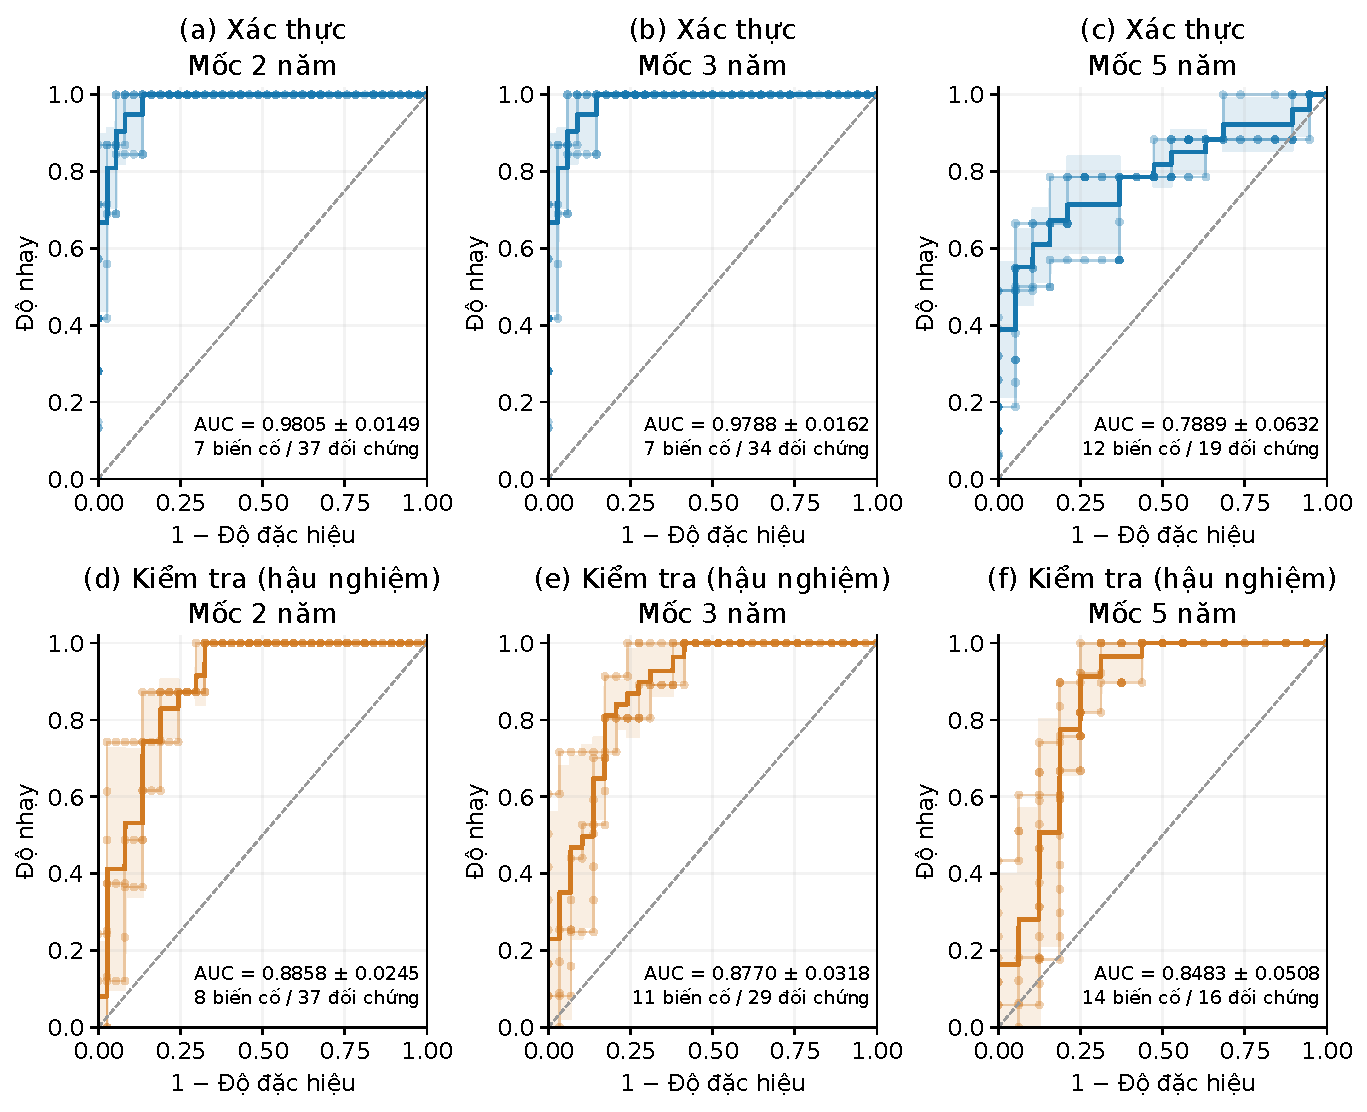
\includegraphics[width=\textwidth]{image/empirical-ipcw-roc.pdf}
\caption{Đường cong ROC có trọng số IPCW của RC-Free tại 2, 3 và 5 năm}
\label{fig:empirical-roc}
\captionsetup{justification=raggedright}
\caption*{Hàng trên: tập xác thực; hàng dưới: tập kiểm tra hậu nghiệm. Đường mảnh và chấm tròn là từng lần chạy; đường đậm là trung bình; vùng tô là $\pm1$ SD. Đường chéo biểu thị mức đoán ngẫu nhiên.}
\end{figure}

\clearpage
\subsection{Phân tầng Kaplan--Meier theo nhóm nguy cơ đồng thuận}
Hình~\ref{fig:survival-km} và Bảng~\ref{tab:km-statistics} đánh giá khả năng tách biệt hai nhóm nguy cơ cao và thấp (phân nhóm bằng ngưỡng trung vị tập huấn luyện và đồng thuận đa số qua ba lần chạy).

\begin{figure}[H]
\centering
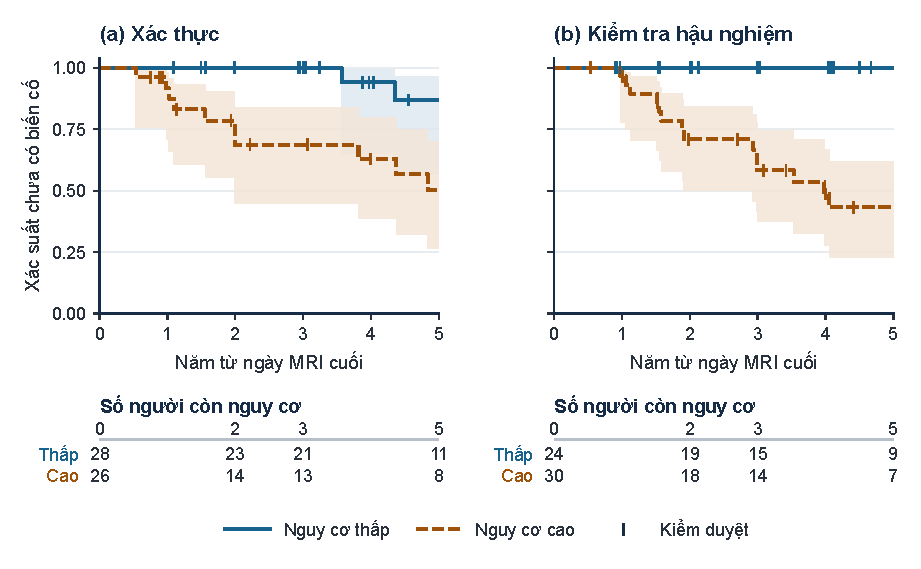
\includegraphics[width=\textwidth]{image/survival-km.pdf}
\caption{Đường cong Kaplan--Meier theo nhóm nguy cơ đồng thuận của RC-Free}
\label{fig:survival-km}
\captionsetup{justification=raggedright}
\caption*{Ô (a): tập xác thực; ô (b): tập kiểm tra hậu nghiệm. Vùng tô là khoảng tin cậy 95\%; dấu gạch dọc đánh dấu thời điểm kiểm duyệt. Bảng dưới trục hoành ghi số người còn nguy cơ tại các mốc thời gian.}
\end{figure}

\begin{table}[H]
\centering\small
\caption[Log-rank và HR theo nhóm nguy cơ]{Log-rank, HR cao/thấp và kiểm tra nguy cơ tỷ lệ (PH).}
\label{tab:km-statistics}
\begin{tabularx}{\linewidth}{@{}Y r r r r@{}}
\toprule
\textbf{Tập} & \textbf{Log-rank p} & \textbf{HR} & \textbf{CI 95\%} & \textbf{p (PH)} \\
\midrule
Xác thực & $0.013360$ & $3.79$ & $1.22$--$11.78$ & $0.103$ \\
Kiểm tra hậu nghiệm & $0.000313$ & $16.17$ & $2.12$--$123.17$ & $0.159$ \\
\bottomrule
\end{tabularx}
\end{table}


Hai đường cong tách biệt rõ nét trên cả hai tập dữ liệu, khẳng định năng lực phân tầng nguy cơ vượt trội của mô hình. Trên tập xác thực, nhóm nguy cơ thấp (28 người) chỉ ghi nhận 4 biến cố, trong khi nhóm nguy cơ cao (26 người) ghi nhận 12 biến cố — gấp ba lần nhóm thấp; kiểm định log-rank xác nhận sự khác biệt có ý nghĩa thống kê (\textbf{$p=0.0134$}), với tỷ số nguy cơ ước tính \textbf{HR = 3.79} (CI 95\%: 1.22--11.78). Trên tập kiểm tra hậu nghiệm, độ tương phản còn mạnh mẽ hơn: trong 24 người thuộc nhóm nguy cơ thấp gần như không ghi nhận ca suy giảm nào trong hơn 5 năm đầu (chỉ duy nhất 1 biến cố sau năm thứ năm), đối lập với 15 biến cố trong 30 người thuộc nhóm nguy cơ cao, đạt \textbf{log-rank $p<0.001$} và \textbf{HR = 16.17} (CI 95\%: 2.12--123.17). Khoảng tin cậy rộng của HR trên tập kiểm tra bắt nguồn trực tiếp từ việc nhóm nguy cơ thấp chỉ có đúng một biến cố làm mẫu số so sánh; ngay cả cận dưới của khoảng tin cậy 95\% vẫn đạt 2.12, cho thấy nhóm nguy cơ cao vẫn có tốc độ tiến triển cao hơn rõ rệt. Đồng thời, phép kiểm tra phần dư Schoenfeld cho $p=0.1031$ trên tập xác thực và $p=0.1592$ trên tập kiểm tra (đều lớn hơn 0.05), chứng tỏ tỷ lệ nguy cơ giữa hai nhóm duy trì ổn định theo thời gian và khẳng định RC-Free là kiến trúc vừa đạt hiệu quả xếp hạng cao nhất, vừa cho khả năng phân tầng sống còn sắc nét và tin cậy nhất trong toàn bộ các thử nghiệm.

\section{Trả lời các câu hỏi nghiên cứu}
\label{sec:rq-results}
Tổng hợp toàn bộ chuỗi thực nghiệm trên, câu trả lời cho năm câu hỏi nghiên cứu ở Bảng~\ref{tab:rq} như sau:

\begin{description}[leftmargin=1.35cm,labelwidth=1.1cm,itemsep=.3em]
\item[RQ1.] \emph{Dữ liệu dọc}: Chuỗi ba lần chụp MRI cải thiện rõ rệt so với chỉ dùng ảnh cuối khi kết hợp T-LSTM với attention, tăng C-index xác thực từ 0.7333 lên \textbf{0.7833} (Bảng~\ref{tab:exploratory}).
\item[RQ2.] \emph{Đa phương thức}: Bổ sung radiomics và dữ liệu lâm sàng bằng ghép nối tiếp tục nâng C-index xác thực lên \textbf{0.8125} (+0.0292 so với chỉ dùng MRI, Bảng~\ref{tab:exploratory}).
\item[RQ3.] \emph{Tương tác cặp so với ghép nối}: Khi giữ cùng trọng số khởi tạo cho các phần chung, phép tích ngoài đạt C-index xác thực trung bình cao hơn ghép nối \textbf{0.0135} (0.8285 so với 0.8149, Bảng~\ref{tab:matched-fusion}).
\item[RQ4.] \emph{Phân rã CP}: CP giảm \textbf{98.38\%} số tham số ở ba lớp song tuyến đầu (90.90\% ở ba khối tương tác; 0.67\% toàn mạng, Bảng~\ref{tab:interaction-parameters}), đổi lại mức giảm nhỏ 0.0066 C-index giữa Full CP và Full Outer-Product (Bảng~\ref{tab:standard-bench}).
\item[RQ5.] \emph{Tinh gọn thành RC-Free}: Khả thi và hiệu quả. Bỏ cặp RC tiết kiệm thêm \textbf{15460 tham số} so với Full CP, rút từ sáu xuống bốn nhánh và đạt C-index xác thực trung bình cao nhất trong bảy cấu trúc CP (\textbf{0.8347}, Bảng~\ref{tab:new-topology}), đồng thời phân tầng nguy cơ có ý nghĩa thống kê trên đường cong Kaplan--Meier (Bảng~\ref{tab:km-statistics}).
\end{description}

\chapter[Thảo luận, kết luận và hướng phát triển]{Thảo luận, kết luận\\và hướng phát triển}
\label{chap:discussion}

\section{Thảo luận các phát hiện chính}
Chuỗi thực nghiệm ở Chương~\ref{chap:results} làm sáng tỏ ba bài học thiết kế đáng chú ý cho bài toán học sâu sống còn đa phương thức trên dữ liệu y tế cỡ mẫu vừa và nhỏ.

Thứ nhất, \emph{hiệu quả nén tham số của phân rã CP cần được nhìn đúng theo từng phạm vi kiến trúc}. Thay lớp chiếu tích ngoài bằng phân rã CP giúp giảm tới \textbf{98.38\%} tham số ở ba lớp song tuyến đầu (từ 229696 xuống 3712) và 90.90\% khi tính cả khối MLP tương tác, nhưng chỉ giảm khoảng 0.67\% tổng tham số toàn mạng vì bộ mã hóa ảnh ResNet-18 3D chiếm phần áp đảo. Điều này có nghĩa là lợi ích lớn nhất của CP trong kiến trúc này không nằm ở việc thu nhỏ dung lượng toàn mạng, mà ở việc \emph{tránh quá khớp cục bộ tại tầng hợp nhất} — nơi dễ phình trọng số nhất khi kết hợp nhiều nguồn đặc trưng trên 251 bệnh nhân huấn luyện. Mức đánh đổi C-index giữa Full CP và Full Outer-Product chỉ là 0.0066, là cái giá hợp lý cho sự tinh gọn ở tầng tương tác.

Thứ hai, \emph{nhiều cặp tương tác hơn không đồng nghĩa với kết quả tốt hơn}. Trong bảy cấu trúc CP có tương tác cặp, RC-Free chỉ giữ hai cặp MR và MC với bốn nhánh phần dư nhưng đạt C-index xác thực trung bình cao nhất (\textbf{0.8347}). Kết quả này nhỉnh hơn Full CP (0.8278) và giảm được 15460 tham số; thậm chí cấu trúc một cặp RC-only cũng đạt 0.8319, cao hơn Full CP. Vì cả ba nguồn dữ liệu vẫn giữ đường truyền gốc qua phần dư có cổng, việc cộng thêm cả ba cặp tương tác có thể gây dư thừa và tăng phương sai ước lượng trên mẫu nhỏ. Khi đặt ảnh MRI làm cầu nối sang radiomics và lâm sàng, RC-Free là cấu trúc gọn nhẹ và hiệu quả nhất.

Thứ ba, \emph{ý nghĩa thực tiễn của phân tầng nguy cơ luôn gắn với cỡ mẫu và số biến cố}. Phân tích Kaplan--Meier cho thấy điểm nguy cơ của RC-Free tách biệt hai nhóm diễn biến: trên tập xác thực đạt log-rank $p=0.0134$ (12/26 so với 4/28 biến cố) và trên tập kiểm tra hậu nghiệm đạt $p<0.001$. Tuy nhiên, khi xét theo từng thời hạn, AUC xác thực tại 2 và 3 năm (0.9805 và 0.9788) chỉ dựa trên 7 biến cố tích lũy. Tại mốc 5 năm, AUC giảm xuống 0.7889 kèm độ lệch chuẩn rộng hơn khi số người còn theo dõi quá 5 năm chỉ còn 19 (Bảng~\ref{tab:horizon-support}).

\section{Giới hạn nghiên cứu}
\label{sec:study-limitations}
Nghiên cứu còn tồn tại bốn giới hạn chính sau:
\begin{enumerate}[itemsep=0.15em,topsep=0.25em]
\item \textbf{Dữ liệu mới dừng ở bộ ADNI, chưa thử nghiệm tại Việt Nam.} Toàn bộ quá trình huấn luyện và đánh giá hiện chỉ sử dụng bộ dữ liệu quốc tế ADNI với tập kiểm chứng còn khiêm tốn (54 người xác thực và 54 người kiểm tra hậu nghiệm). Mô hình chưa được thu thập và kiểm thử trên dữ liệu thực tế từ các bệnh viện lớn ở Việt Nam, nơi thiết bị chụp MRI, quy trình đo lâm sàng và đặc điểm người bệnh có thể khác biệt.
\item \textbf{Thiết kế mốc thời gian hồi cứu.} Thời gian sống còn $t_i$ được tính từ ngày chụp MRI thứ ba $p_i$, nhưng quy tắc lọc mẫu lại giữ những người chưa tiến triển đến hết mốc 18 tháng $L_i$ (nên có nguy cơ sai lệch thời gian bất tử nếu diễn giải như dự báo ngay tại ngày chụp $p_i$ \cite{suissa2008immortal}). Ngoài ra, cửa sổ ghép $\pm90$ ngày làm 57 người có điểm MMSE hoặc CDR gắn với lần chụp cuối thực tế được đo sau ngày $p_i$ (Mục~\ref{sec:data-split}), khiến kết quả hiện tại phù hợp hơn cho đánh giá trên nhóm hồi cứu.
\item \textbf{Thang đo đầu vào và định nghĩa biến cố cùng dùng MMSE và CDR.} Dù hai giai đoạn đo được tách biệt trước và sau mốc 18 tháng, việc cùng dựa vào ngưỡng điểm MMSE và CDR để xác định biến cố vẫn tạo sự phụ thuộc vào hai thang đo này; mô hình chưa được đối chiếu với chẩn đoán lâm sàng độc lập hay các xét nghiệm sinh học chuyên sâu hơn.
\item \textbf{Đầu ra mới dừng ở mức xếp hạng nguy cơ.} Điểm $\eta_i$ của mô hình Cox cho biết ai có nguy cơ tiến triển sớm hơn ai, nhưng chưa quy đổi trực tiếp thành xác suất tiến triển cụ thể theo phần trăm cho từng bệnh nhân và chưa đo tốc độ xử lý thực tế trên máy tính tại bệnh viện.
\end{enumerate}

\section{Hướng phát triển}
Từ các giới hạn trên, khóa luận có thể mở rộng theo ba hướng thực tế:
\begin{enumerate}[itemsep=0.15em,topsep=0.25em]
\item \emph{Thử nghiệm trên dữ liệu bệnh viện tại Việt Nam}: Phối hợp thu thập dữ liệu theo dõi dọc từ các bệnh viện lớn trong nước để kiểm chứng, hiệu chỉnh mô hình phù hợp với bệnh nhân Việt Nam và bổ sung thêm các nguồn thông tin xét nghiệm sẵn có.
\item \emph{Hoàn thiện thiết kế dự báo theo mốc thời gian}: Giới hạn chặt dữ liệu lâm sàng đến trước ngày chụp cuối $p_i$ hoặc áp dụng thiết kế dự báo tại mốc cố định $L_i$ \cite{vanhouwelingen2007dynamic} để loại bỏ hoàn toàn độ lệch thời gian giữa đầu vào và kết cục.
\item \emph{Quy đổi xác suất cá thể hóa và hỗ trợ giải thích}: Ước lượng thêm hàm sống còn nền \cite{kvamme2019time} để chuyển điểm nguy cơ thành xác suất tiến triển theo từng năm, kết hợp phân tích trọng số attention và cổng điều tiết nhằm giúp bác sĩ dễ theo dõi cơ sở dự báo và đo lường thời gian chạy thực tế khi triển khai ứng dụng.
\end{enumerate}

\section{Kết luận}
Tiên lượng tiến triển ở người mắc suy giảm nhận thức nhẹ đòi hỏi không chỉ theo dõi diễn biến qua nhiều lần khám, mà còn kết hợp hài hòa giữa hình ảnh cấu trúc não, đặc trưng định lượng và đánh giá lâm sàng. Trên tập dữ liệu hồi cứu gồm 359 người tham gia ADNI với ba mốc thăm khám, khóa luận đã xây dựng một quy trình phân tích sống còn đa phương thức hoàn chỉnh tích hợp ảnh MRI 3D, radiomics toàn não và thang điểm MMSE/CDR. Các thực nghiệm đối chứng khẳng định từng bước đóng góp của thiết kế: chuỗi MRI dọc với T-LSTM và attention vượt trội so với ảnh đơn thời điểm, kết hợp đủ ba nguồn nâng cao rõ rệt năng lực xếp hạng nguy cơ, và mô hình hóa tương tác song tuyến theo cặp khai thác mối liên hệ giữa các nguồn hiệu quả hơn phép ghép nối thông thường.

Kiến trúc \textbf{RC-Free} kết hợp hai bước tinh giản: phân rã tensor CP hạng thấp giúp giảm 98.38\% tham số ở ba lớp song tuyến đầu, và lược bỏ cặp tương tác trực tiếp RC giúp tiết kiệm thêm 15460 tham số so với Full CP mà vẫn giữ đủ ba nguồn đầu vào. Trên tập xác thực, RC-Free đạt C-index trung bình cao nhất trong bảy cấu trúc CP ($0.8347\pm0.0237$) và phân tầng có ý nghĩa thống kê hai nhóm nguy cơ sống còn ($p=0.0134$). Kết quả này cho thấy kết hợp tham số hóa hạng thấp với chọn lọc cặp tương tác hợp lý là hướng đi gọn nhẹ và khả thi cho tiên lượng đa phương thức trên dữ liệu y tế cỡ mẫu hạn chế.

\clearpage
\appendix
\begingroup
\renewcommand{\chaptername}{Phụ lục}
\titleformat{\chapter}[hang]{\normalfont\bfseries\Large}{\chaptername\ \thechapter.}{0.5em}{}
\titlespacing*{\chapter}{0pt}{0pt}{12pt}
\addtocontents{toc}{\protect\renewcommand{\protect\cftchappresnum}{Phụ lục~}}
\begin{landscape}
\chapter{Sơ đồ tổng hợp quy trình RC-Free}
\label{app:master-pipeline}
\begin{figure}[H]
\centering
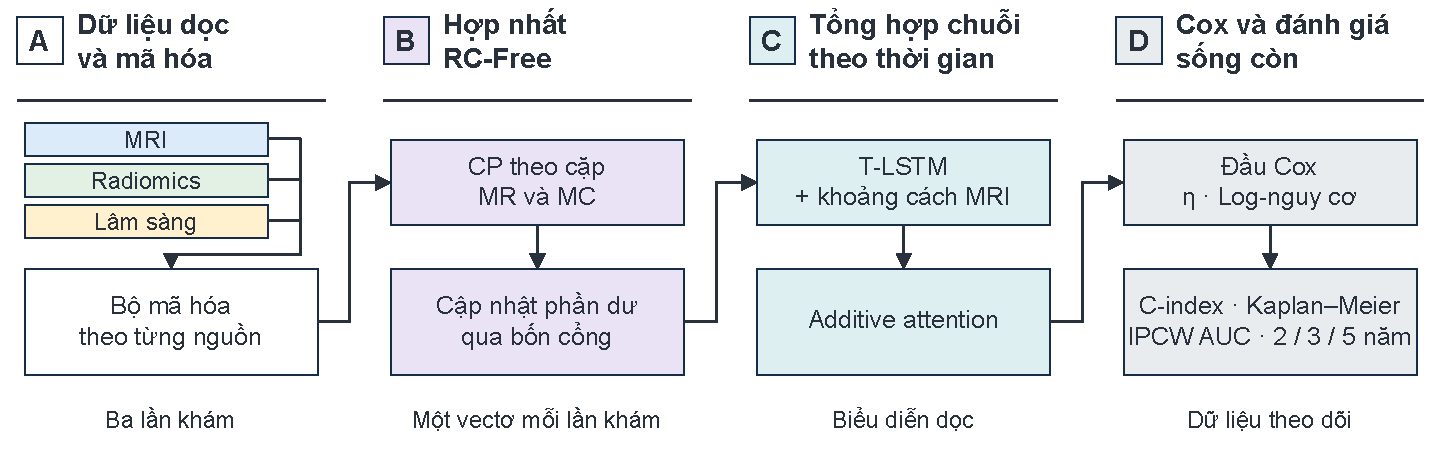
\includegraphics[width=\linewidth,height=11.5cm,keepaspectratio]{image/master-pipeline.pdf}
\caption[Quy trình RC-Free từ đầu vào đến đánh giá]{Mô hình mã hóa dữ liệu của ba lần khám theo từng nguồn (A), tính tương tác MR và MC để cập nhật biểu diễn qua các nhánh phần dư (B), rồi tổng hợp chuỗi theo thời gian (C). Khối Cox tạo điểm log-nguy cơ dùng trong đánh giá sống còn (D).}
\label{fig:master-pipeline}
\end{figure}
\end{landscape}
\endgroup


\clearpage
\phantomsection
\addcontentsline{toc}{chapter}{TÀI LIỆU THAM KHẢO}
\renewcommand{\bibname}{TÀI LIỆU THAM KHẢO}
\begingroup
\renewcommand{\bibfont}{\renewcommand{\baselinestretch}{1.15}\fontsize{12}{14}\selectfont}
\setlength{\bibsep}{0pt}
\bibliographystyle{thesisrefs}
\bibliography{references}
\endgroup

\end{document}
